%% abtex2-modelo-trabalho-academico.tex, v<VERSION> laurocesar
%% Copyright 2012-2015 by abnTeX2 group at http://www.abntex.net.br/ 
%%
%% This work may be distributed and/or modified under the
%% conditions of the LaTeX Project Public License, either version 1.3
%% of this license or (at your option) any later version.
%% The latest version of this license is in
%%   http://www.latex-project.org/lppl.txt
%% and version 1.3 or later is part of all distributions of LaTeX
%% version 2005/12/01 or later.
%%
%% This work has the LPPL maintenance status `maintained'.
%% 
%% The Current Maintainer of this work is the abnTeX2 team, led
%% by Lauro César Araujo. Further information are available on 
%% http://www.abntex.net.br/
%%
%% This work consists of the files abntex2-modelo-trabalho-academico.tex,
%% abntex2-modelo-include-comandos and abntex2-modelo-references.bib
%%

% ------------------------------------------------------------------------
% ------------------------------------------------------------------------
% abnTeX2: Modelo de Trabalho Academico (tese de doutorado, dissertacao de
% mestrado e trabalhos monograficos em geral) em conformidade com 
% ABNT NBR 14724:2011: Informacao e documentacao - Trabalhos academicos -
% Apresentacao
% ------------------------------------------------------------------------
% ------------------------------------------------------------------------

\documentclass[
	% -- opções da classe memoir --
	12pt,				% tamanho da fonte
	openright,			% capítulos começam em pág ímpar (insere página vazia caso preciso)
	twoside,			% para impressão em recto e verso. Oposto a oneside
	a4paper,			% tamanho do papel. 
	% -- opções da classe abntex2 --
	%chapter=TITLE,		% títulos de capítulos convertidos em letras maiúsculas
	%section=TITLE,		% títulos de seções convertidos em letras maiúsculas
	%subsection=TITLE,	% títulos de subseções convertidos em letras maiúsculas
	%subsubsection=TITLE,% títulos de subsubseções convertidos em letras maiúsculas
	% -- opções do pacote babel --
	english,			% idioma adicional para hifenização
%	french,				% idioma adicional para hifenização
%	spanish,			% idioma adicional para hifenização
	brazil				% o último idioma é o principal do documento
	]{style/abntex2}

% ---
% Pacotes básicos 
% ---
\usepackage{lmodern}			% Usa a fonte Latin Modern			
\usepackage[T1]{fontenc}		% Selecao de codigos de fonte.
\usepackage[utf8]{inputenc}		% Codificacao do documento (conversão automática dos acentos)
\usepackage{lastpage}			% Usado pela Ficha catalográfica
\usepackage{indentfirst}		% Indenta o primeiro parágrafo de cada seção.
\usepackage{color}				% Controle das cores
\usepackage{graphicx}			% Inclusão de gráficos
\usepackage{microtype} 			% para melhorias de justificação
\usepackage{enumitem}
\setlist{nosep}
% ---
		
% ---
% Pacotes adicionais, usados apenas no âmbito do Modelo Canônico do abnteX2
% ---
\usepackage{lipsum}				% para geração de dummy text
% ---

% ---
% Pacotes de citações
% ---
\usepackage[brazilian,hyperpageref]{backref}	 % Paginas com as citações na bibl
\usepackage[alf]{style/abntex2cite}	% Citações padrão ABNT

% --- 
% CONFIGURAÇÕES DE PACOTES
% --- 

% ---
% Configurações do pacote backref
% Usado sem a opção hyperpageref de backref
\renewcommand{\backrefpagesname}{Citado na(s) página(s):~}
% Texto padrão antes do número das páginas
\renewcommand{\backref}{}
% Define os textos da citação
\renewcommand*{\backrefalt}[4]{
	\ifcase #1 %
		No citation on text.%
	\or
		Cited on page #2.%
	\else
		Cited #1 times on pages #2.%
	\fi}%

\newcounter{hypothesisno}
\DeclareRobustCommand{\hypothesis}[1]{H\refstepcounter{hypothesisno}\thehypothesisno\label{#1}}
% ---

% ---
% Informações de dados para CAPA e FOLHA DE ROSTO
% ---
\titulo{Advancing on Use of Open Data Through Data Literacy and Semantic Enhancement of Metadata}
\autor{Alan Freihof Tygel}
\local{Rio de Janeiro}
\data{2016}
\orientador{Maria Luiza Machado Campo}
\coorientador{Sören Auer}
\instituicao{%
  Universidade Federal do Rio de Janeiro
  \par
  Instituto de Matemática \& Instituto Tércio Pacitti de Aplicações e 
  \par Pesquisas Computacionais, Programa de Pós-Graduação em Informática}
\tipotrabalho{Tese (Doutorado)}
% O preambulo deve conter o tipo do trabalho, o objetivo, 
% o nome da instituição e a área de concentração 
\preambulo{Tese de Doutorado submetida ao Corpo Docente do Programa de Pós-Graduação em Informática do Instituto de Matemática e Instituto Tércio Pacitti de Aplicações e Pesquisas Computacionais da Universidade Federal do Rio de Janeiro, como parte dos requisitos necessários para obtenção do título de Doutor em Informática.}
% ---


% ---
% Configurações de aparência do PDF final

% alterando o aspecto da cor azul
\definecolor{blue}{RGB}{41,5,195}

% informações do PDF
\makeatletter
\hypersetup{
     	%pagebackref=true,
		pdftitle={\@title}, 
		pdfauthor={\@author},
    	pdfsubject={\imprimirpreambulo},
	    pdfcreator={LaTeX with abnTeX2},
		pdfkeywords={abnt}{latex}{abntex}{abntex2}{trabalho acadêmico}, 
		colorlinks=true,       		% false: boxed links; true: colored links
    	linkcolor=blue,          	% color of internal links
    	citecolor=blue,        		% color of links to bibliography
    	filecolor=magenta,      		% color of file links
		urlcolor=blue,
		bookmarksdepth=4
}
\makeatother
% --- 

% --- 
% Espaçamentos entre linhas e parágrafos 
% --- 

% O tamanho do parágrafo é dado por:
\setlength{\parindent}{1.3cm}

% Controle do espaçamento entre um parágrafo e outro:
\setlength{\parskip}{0.2cm}  % tente também \onelineskip

% ---
% compila o indice
% ---
\makeindex
% ---

% ----
% Início do documento
% ----
\begin{document}

% Seleciona o idioma do documento (conforme pacotes do babel)
\selectlanguage{english}
%\selectlanguage{brazil}

% Retira espaço extra obsoleto entre as frases.
\frenchspacing 

% ----------------------------------------------------------
% ELEMENTOS PRÉ-TEXTUAIS
% ----------------------------------------------------------
% \pretextual

% ---
% Capa
% ---
\imprimircapa
% ---

% ---
% Folha de rosto
% (o * indica que haverá a ficha bibliográfica)
% ---
\imprimirfolhaderosto*
% ---

% ---
% Inserir a ficha bibliografica
% ---

% Isto é um exemplo de Ficha Catalográfica, ou ``Dados internacionais de
% catalogação-na-publicação''. Você pode utilizar este modelo como referência. 
% Porém, provavelmente a biblioteca da sua universidade lhe fornecerá um PDF
% com a ficha catalográfica definitiva após a defesa do trabalho. Quando estiver
% com o documento, salve-o como PDF no diretório do seu projeto e substitua todo
% o conteúdo de implementação deste arquivo pelo comando abaixo:
%
% \begin{fichacatalografica}
%     \includepdf{fig_ficha_catalografica.pdf}
% \end{fichacatalografica}

\begin{fichacatalografica}
	\sffamily
	\vspace*{\fill}					% Posição vertical
	\begin{center}					% Minipage Centralizado
	\fbox{\begin{minipage}[c][8cm]{13.5cm}		% Largura
	\small
	%\imprimirautor
	Tygel, Alan Freihof
	
	T977x \hspace{0.5cm} \imprimirtitulo  / \imprimirautor. --
	\imprimirlocal, \imprimirdata-
	
	\hspace{0.5cm} \pageref{LastPage} p. : il. (algumas color.) ; 30 cm.\\
	
	\hspace{0.5cm} \imprimirorientadorRotulo~\imprimirorientador

	\hspace{0.5cm} \imprimircoorientadorRotulo~\imprimircoorientador
	
	\hspace{0.5cm}
	\parbox[t]{\textwidth}{\imprimirtipotrabalho~--~\imprimirinstituicao,
	\imprimirdata.}\\
	
	\hspace{0.5cm}
		1. Open Data
		2. Semantic Web
		3. Metadata
		4. Data Literacy
		I. Campos, Maria Luiza Machado, orient.
		II. Auer, Sören, coorient.
		III. Título 			
	\end{minipage}}
	\end{center}
\end{fichacatalografica}
% ---

% ---
% Inserir folha de aprovação
% ---

% Isto é um exemplo de Folha de aprovação, elemento obrigatório da NBR
% 14724/2011 (seção 4.2.1.3). Você pode utilizar este modelo até a aprovação
% do trabalho. Após isso, substitua todo o conteúdo deste arquivo por uma
% imagem da página assinada pela banca com o comando abaixo:
%
% \includepdf{folhadeaprovacao_final.pdf}
%
\begin{folhadeaprovacao}

  \begin{center}
    {\ABNTEXchapterfont\large\imprimirautor}

    \vspace*{\fill}\vspace*{\fill}
    \begin{center}
      \ABNTEXchapterfont\bfseries\Large\imprimirtitulo
    \end{center}
    \vspace*{\fill}
    
    \hspace{.45\textwidth}
    \begin{minipage}{.5\textwidth}
        \imprimirpreambulo
    \end{minipage}%
    \vspace*{\fill}
   \end{center}
        
   Trabalho aprovado. \imprimirlocal, 24 de novembro de 2012:

   \assinatura{\textbf{\imprimirorientador} \\ Orientador} 
   \assinatura{\textbf{\imprimircoorientador} \\ Co-orientador} 
   \assinatura{\textbf{Bernardete Farias Loscio} \\ Examinadora}
   \assinatura{\textbf{Maria Claudia Cavalcanti} \\ Examinadora}
   \assinatura{\textbf{Marcelo Firpo de Souza Porto} \\ Examinador}
   \assinatura{\textbf{Marcos Borges} \\ Examinador}
   \assinatura{\textbf{Jonice de Oliveira Sampaio} \\ Examinadora}
      
   \begin{center}
    \vspace*{0.5cm}
    {\large\imprimirlocal}
    \par
    {\large\imprimirdata}
    \vspace*{1cm}
  \end{center}
  
\end{folhadeaprovacao}
% ---

% ---
% Dedicatória
% ---
%\begin{dedicatoria}
%   \vspace*{\fill}
%   \centering
%   \noindent
%   \textit{ Este trabalho é dedicado às crianças adultas que,\\
%   quando pequenas, sonharam em se tornar cientistas.} \vspace*{\fill}
%\end{dedicatoria}
% ---

% ---
% Agradecimentos
% ---
%\begin{agradecimentos}
%Os agradecimentos principais são direcionados à Gerald Weber, Miguel Frasson,
%Leslie H. Watter, Bruno Parente Lima, Flávio de Vasconcellos Corrêa, Otavio Real
%Salvador, Renato Machnievscz\footnote{Os nomes dos integrantes do primeiro
%projeto abn\TeX\ foram extraídos de
%\url{http://codigolivre.org.br/projects/abntex/}} e todos aqueles que
%contribuíram para que a produção de trabalhos acadêmicos conforme
%as normas ABNT com \LaTeX\ fosse possível.

%Agradecimentos especiais são direcionados ao Centro de Pesquisa em Arquitetura
%da Informação\footnote{\url{http://www.cpai.unb.br/}} da Universidade de
%Brasília (CPAI), ao grupo de usuários
%\emph{latex-br}\footnote{\url{http://groups.google.com/group/latex-br}} e aos
%novos voluntários do grupo
%\emph{\abnTeX}\footnote{\url{http://groups.google.com/group/abntex2} e
%\url{http://www.abntex.net.br/}}~que contribuíram e que ainda
%contribuirão para a evolução do \abnTeX.

%\end{agradecimentos}
% ---

% ---
% Epígrafe
% ---
%\begin{epigrafe}
%    \vspace*{\fill}
%	\begin{flushright}
%		\textit{``Não vos amoldeis às estruturas deste mundo, \\
%		mas transformai-vos pela renovação da mente, \\
%		a fim de distinguir qual é a vontade de Deus: \\
%		o que é bom, o que Lhe é agradável, o que é perfeito.\\
%		(Bíblia Sagrada, Romanos 12, 2)}
%	\end{flushright}
%\end{epigrafe}
%% ---

% ---
% RESUMOS
% ---

% resumo em português
\setlength{\absparsep}{18pt} % ajusta o espaçamento dos parágrafos do resumo
\begin{resumo}[Resumo]
A publicação extensiva de dados em formatos abertos na Internet parece ser uma tendência irreversível.
No caso de governos, pressões da sociedade por mais transparência vem fazendo com que cada vez mais, administrações públicas facilitem acessos aos dados de governo criando centrais únicas de acesso.
Estes repósitorios centrais de dados, ou portais de dados abertos, têm como objetivo ser um ponto de encontro entre o governo e cidadãos e cidadãs que desejam acessar dados públicos.
Espera-se com isso uma maior transparência das administrações públicas, que por sua vez alimenta a democracia com a população bem informada, e inibe desvios de recursos através da possibilidade de uma inspeção aberta ao público.
Junto às grandes expectativas geradas pelas políticas de dados abertos, verifica-se também uma ampla gama de problemas que ainda retardam o crescimento das iniciativas. 
No decorrer da pesquisa relacionada a esta tese, dois problemas chamaram a atenção: (i) a falta de organização conceitual dos portais de dados abertos e (ii) as dificuldades do público em geral em lidar com os dados.
Deste modo, esta tese busca trazer uma contribuição para o campo dos dados abertos propondo abordagens para ambos os problemas.
Administradores dos portais de dados abertos utilizam diversos tipos de metadados para organizar seus conjuntos de dados, sendo o mais importante as tags.
Entretanto, o processo de tageamento é sujeito a diversos problemas, como sinonimia, ambiguidade ou incoerência, entre outros. 
Como demonstrado por nossa análise empírica dos ODPs, estes problemas são atualmente prevalente na maior parte dos portais, e efetivamente dificultam o reuso dos dados abertos. 
Face a estes problemas, nesta tese foi desenvolvida e implemenatada uma abordagem para reconcialição de tags em portais de dados abertos, incluindo ações locais relacionadas individualmente aos portais, e ações globais para adição de uma camada de metadados semânticos acima dos portais individuais.
Diversos estudo apontam ainda que, dentro das políticas de dados abertos adotadas pelos governos, há um foco maior na publicação de dados, e uma menor atenção à capacidade de uso destes dados pelo público.
Assim, ainda que os dados sejam publicados, é necessário que haja um público capacitado para lidar eles.
Do contrário, corre-se o risco de criar uma elite capaz de tirar proveito destas informações, e aprofundar ainda mais a exclusão digital, sobretudo em países com o Brasil.
Neste sentido, apresentamos nesta tese uma abordagem para alfabetização em dados, inspirada na pedagodia da educação popular e na técnica de pequisa-ação participativa.
Deste modo, espera-se com essa tese contribuir com o avanço da democratização das informações, contextualizando de forma mais adequada a publicação de dados abertos, e permitindo um uso mais ampliado pela população.

\textbf{Palavras-chave}: Dados Abertos. Portal de Dados Abertos. Conciliação de Metadados. Enriquecimento Semântico. Alfabetização em Dados.
\end{resumo}



% resumo em inglês
%\begin{englishabstract}{Colocar aqui o título da dissertação em inglês}{coloque aqui as palavras-chave em inglês, separadas por vírgula}
%Avançando no Uso de Dados Abertos Através do Enriquecimento Semânticos de Metadados e da Alfabetização em Dados

\begin{resumo}[Abstract]
 \begin{otherlanguage*}{english}
The extensive publishing of data in open formats on the Web seems to be an irreversible tendency.
Regarding governments, claims for more transparency coming from the civil society are forcing public administrations to ease the access to government data, mostly through central data repositories.
These data repositories, or Open Data Portals (ODPs), have the objective of being a meeting point between government and citizens willing to access public data.
Hence, it is expected a greater transparency of public administrations, which in turn feed democracy with a well informed population, and inhibits corruption through the possibility of open scrutiny by the public.
Alongside the great expectations created by the open data policies, we also verify a wide range of problems which still hinder a more effective growing of the open data initiatives.
During the research related to this thesis, two problems called the attention: (i) the lack of conceptual organization of the open data portals, and (ii) the difficulties of the general public for dealing with data.
Thus, this thesis expects to bring a contribution for the field of open data by proposing approaches for both problems.
ODP managers use several types of metadata to organize the datasets, one of the most important ones being the tags.
However, the tagging process is subject to many problems, such as synonyms, ambiguity or incoherence, among others.
As our empiric analysis of ODPs shows, these issues are currently prevalent in most ODPs and effectively hinders the reuse of Open Data.
In order to address these problems, we develop and implement an approach for tag reconciliation in Open Data Portals, encompassing local actions related to individual portals, and global actions for adding a semantic metadata layer above individual portals.
Several studies attest that, on the open data policies adopted by governments, there is a greater attention on data publishing, while enhancing the capacity of people for using these data remains in background. 
Thus, even if data are published, it is necessary to have an empowered society to deal with it.
Otherwise, there is a risk of creating an elite able to profit from these information, deepening even more the digital divide, especially in countries like Brazil.
In order to tackle this matter, we present in this thesis an approach for data literacy, inspired in the pedagogy of popular education and in the participatory action-research technique.
It is expected that this thesis contribute with and advance in the democratisation of information, contextualizing in a more adequate form the publication of open data, and allowing its use by a broader part of the population.


\textbf{Keywords}: Open Data. Open Data Portal. Metadata Reconciliaton. Semantic Lifting. Data Literacy.
 \end{otherlanguage*}
\end{resumo}




% ---

% ---
% inserir lista de ilustrações
% ---
\pdfbookmark[0]{\listfigurename}{lof}
\listoffigures*
\clearpage
% ---

% ---
% inserir lista de tabelas
% ---
\pdfbookmark[0]{\listtablename}{lot}
\listoftables*
\clearpage
% ---

% ---
% inserir lista de abreviaturas e siglas
% ---
% Examples

\begin{siglas}
  \item [CSO] Civil Socieity Organization
  \item [FOIA] Freedom of Information Act
  \item [ICT] Information and Communications Technology
  \item [LOD] Linked Open Data
  \item [NGO] Non-Governmental Organization
  \item [ODP] Open Data Portal
  \item [OGD] Open Government Data
  \item [OGP] Open Government Partnership
  \item [STODaP] Semantic Tags for Open Data Portals
\end{siglas}


% ---

% ---
% inserir o sumario
% ---
\pdfbookmark[0]{\contentsname}{toc}
\tableofcontents*
\clearpage
% ---

\textual
% ----------------------------------------------------------
% ELEMENTOS TEXTUAIS
% ----------------------------------------------------------


\chapter{Introduction}

This thesis is essentially about open data.
Given the growing importance of the topic, open data is discussed through several points of views.
Although looking at it from a Computer Science perspective, it was not possible to skip political, social and economical aspects while discussing the topic.
This work should thus be regarded as a multidisciplinary effort to contribute to a field that is heavily related to Computer Science, but far from being restricted to it.

In this introductory chapter, some motivations behind the topic of open data are briefly exposed, highlighting selected problems observed in the literature.
The hypothesis from where this thesis starts are posed, as well as the objectives that we aim to achieve with this work.
We further explain the methodology used in order to develop this thesis, and finally describe the structure of the rest of this text.

\section{Motivation}
% * crescimento do open data
Current numbers about the open data scene leave no doubt about the central importance of this topic in contemporary society.
The Open Data Index\footnote{Available at \url{http://index.okfn.org/place/}.} monitored in 2015 open datasets published by 122 countries all over the world, on topics related to budget, national statistics, procurements, maps and many others.
Regarding the European landscape, the {Open Data Monitor\footnote{Available at \url{http://opendatamonitor.eu}.} counts 173 open data catalogues in the continent, which sums an amount of 1472 GB of data.

The movement towards opening datasets has its roots related to a series of access to information laws. 
According to the right2info.org\footnote{Available at \url{http://right2info.org}.} platform, these are laws that ``establish the right and procedures for the public to request and receive government-held information''.
\citeonline{Vleugels2012} presents a comprehensive list of 273 Freedom of Information Acts (FOIA), being 93 of national, 180 of sub-national and 3 of international scope.
Even though the first occurrence of this kind of law dates from 1766, in Sweden, the vast majority of them were created after the year 2000.

It is no coincidence that 9 years later, United States and United Kingdom launched their Open Data Portals (ODPs), a one-stop-shop for publishing and consuming government data.
Nowadays, several countries have already implemented their ODPs, together with numerous states and municipalities.
Universities and research centres are also joining strategies for putting data available on the Web.
More than 1600 ODPs were surveyed by OpenDataSoft\footnote{Available at \url{https://www.opendatasoft.com}.}.
The potential of changing the very basis of democratic processes took the United Nations (UN) to coin the term \emph{Data Revolution} to designate ``the new world of data, a world in which data are bigger, faster and more detailed than ever before''~\cite[p.4]{DataRevolutionGroup2014}.
Still according to the UN, these data is ``creating unprecedented possibilities for informing and transforming society and protecting the environment''~\cite[p.4]{DataRevolutionGroup2014}.

A study by \citeonline{Huijboom2011} comparing national open data strategies of five countries analysed their public policies programmes and key motivations behind publishing open data.
Authors defined three main categories of motivations:
\begin{itemize}
	\item Increase democratic control and political participation, i.e., open data could empower citizens on exercising their democratic rights;
	\item Foster service and product innovation, i.e., open data could generate new opportunities for innovation on the public and private sector. Under this topic, it has been recently stated that “Open data can help unlock U\$3 trillion to U\$5 trillion in economic value annually” \cite{Manyika2013}.
	\item Strengthen law enforcement, i.e., open data could enable citizen involvement and enable the development of security application.
\end{itemize}

While the big numbers and great expectations about open data may generate an enthusiastic hope that this movement will solve many problems of the society, there are also critique voices claiming that the promises are still far from being realised, and also that there are some hidden threats that should be alerted.
The problems of open data are the subject of next section.

\section{Not Only Advantages -- Open Data Impediments}

In front of such a big hope regarding the benefits of opening datasets, several authors have also dedicated themselves to analyse open data from a critical point of view \cite{Zuiderwijk2012, Zuiderwijk2014, Gurstein2011, Bates2014, Roseira2016, Parycek2016, Davies2012b}
\footnote{Open data problems will be deeper analysed in \autoref{sec:problems}.
For the purposes of this Introduction, only the most relevant to this work will be detailed.}.

Among them, it is possible to divide open data criticism in two categories: (i) \emph{Problems}, i.e., technological and political implementation failures that prevent open data to achieve their desired goals, and (ii) \emph{Perils}, i.e., unexpected outcomes of open data implementation that are negative for the society as a whole, or specific groups.

Regarding the Problems, \citeonline{Zuiderwijk2012}, in a very complete work, collected 118 socio-technical impediments for use of open data from interviews, workshops and literature.
Some cited impediments were ``absence of commonly agreed metadata'', ``insufficiency of metadata'', ``the lack of interoperability'' and ``difficulty in searching and browsing data'', showing that data organization is great challenge for open data.

The open data organization challenge can be subdivided into two aspects: 1) structuring and organizing the datasets themselves and 2) providing well-structured and organized metadata for the datasets.

The first aspect has been recently approached using the Linked Open Data (LOD) paradigm \cite{Berners-Lee2006}.
In short, this approach aims to semantically enrich data by giving unique identifiers (Uniform Resource Identifier - URIs) to elements of a dataset, and linking these identifiers to commonly agreed knowledge bases, or web ontologies.
The process of connecting isolated datasets to the LOD cloud is called semantic lifting, and was applied to open datasets by~\citeonline{DBLP:conf/i-semantics/ErmilovAS13} and~\citeonline{Ding2011325}, who tried to build general strategies for putting large open government datasets in the Link Open Data (LOD) cloud.

Regarding the second aspect, the Data Catalog Vocabulary (DCAT)\footnote{Available at \url{http://www.w3.org/TR/vocab-dcat/}}~\cite{conf/i-semantics/CyganiakMP10} was developed to provide standardized metadata for open data catalogues.
If DCAT succeeds in providing a standard structure for describing open datasets, e.g., defining fields such as \texttt{dcat:title}, \texttt{dcat:description}, \texttt{dcat:keyword} and \texttt{dcat:theme}, harmonizing the content of these fields is out its scope.
This means that, if we have for Dataset 1 \texttt{dcat:theme spending plan}, and for Dataset 2 \texttt{dcat:theme budget}, both are not linked, although they are dealing with the same subject.


Besides the data organization challenge, another commonly cited impediment to the use of open data is the individuals and groups' lack of capacity for dealing with open data.
There has been a recently growing consensus on defining the skills of consuming, publishing and understanding data under the concept of \emph{Data Literacy}.

As observed by~\citeonline{Bhargava2015}, one of the first mentions to the term \emph{Data Literacy} called the attention for its importance on the context of evaluation of information, together with  Information Literacy and Statistical Literacy. 
In 2004, Schield reinforced the importance of teaching these three literacies for ``students who need to critically evaluate information in arguments'' \cite[p.1]{Schield2004}.

Although not directly mentioning  the term Data Literacy, the previously cited collection of open data impediments~\cite{Zuiderwijk2012} dedicates a section for problems related to \emph{understand ability}.
Among them we find, for example, ``Lack of skills and capabilities to use the data and'' and ``Lack of knowledge about how to interpret the data'', which relate directly to the topic of Data Literacy.

\section{Hypothesis}

In the light of open data theoretical benefits, and the impediments and perils that hinder the achievement of these benefits, we formulate a hypothesis in order to guide the development of this thesis:

% \noindent\textbf{\hypothesis{hyp:dataliteracy}:} ; >> motivação

% confirme que abordagem de soluçao está correta, mas foi mais exploração do problema

\noindent\textbf{\hypothesis{hyp:tagging}:} \emph{Enhancing the organization of open data repositories leads to better find ability of open data.}

% Both hypothesis are inspired in the problems highlighted above.

The hypothesis puts in evidence the data organization problem with the aim of making data more easily available.
It assumes that, if by some means, data repositories could be better organized, data would be more easily accessible by a broader audience.

The first part of H1 -- enhancing the organization of open data repositories -- assumes that open data repositories, or ODPs, exist, and that they are not organized.
Although not exclusively, ODPs are mostly run by governments willing to publish public data, which are also called Open Government Data (OGD).
Our aim is not to develop an exclusive approach for the government context.
However, because most of data available is related to OGD, a bias on this direction can be introduced.
Thus, the existence of ODPs is clear from the first section of this Introduction, and organization problems will be clarified during this text, specifically in \autoref{sec:problems} and \autoref{chap:relworks}.

The second part of H1 -- better find ability of open data -- is related to people wanting to access data.
The first assumption is that data consumers exists, i.e., that there is a demand from the society for open data.
Several works point out the missing focus on users, or data consumers.
Topics regarding open data demand and motivations are detailed in the next chapter, but it is worth mentioning here the work by \citeonline{Davies2012}. 
It describes a survey about the different uses of open data, and gives a more realistic perspective on how people really use data.
The second assumption is that people currently have problems in finding those data.
Reports of problems on finding open data are also available on the literature.
\citeonline{Zuiderwijk2012} summarizes 6 categories of find ability impediments, collected from the literature, workshops and interviews.

Hypothesis H1 goes only until the point when data is found.
But what happens after users get access to the desired open dataset?

Solving the organization problem of open data will not make it more accessible alone.
Increasing the level of data literacy on the society is also of paramount importance in order to democratize access to data, and their claimed benefits.
Otherwise, there is a serious risk of creating a ``Data Divide'', i.e., extending the inequalities of our society to the open data access and thus \emph{empowering the empowered}, as stated by \citeonline{Gurstein2011}.
Although not formulated as a hypothesis, mainly because of our lack of instruments to validate it, we assume in this thesis that an increase on the collective level of data literacy could lead to a democratisation of access and benefits of open data.
Thus, as a motivation of our work, we understand and assume the importance of gradually moving from a current scenario where the society is exposed to data filtered and explained by intermediaries, to another where people can critically read, understand and even produce data themselves.

\section{Objective}

Our aim in this thesis is to develop an approach to enhance the organization of open data repositories, with the perspective of facilitating access to data, and consequently improving the realisation of open data benefits in a democratic way.
In order to accomplish this main target, we formulate as specific objectives (SO):
\begin{enumerate}
	\item To provide an overview on the state of the art regarding the open data landscape;
	\item To investigate in which extent Data Literacy efforts can contribute to democratisation of access to open data;
	\item To systematise literature efforts on semantically enhancing open data descriptors;
	\item To analyse the state of the practice on metadata usage on the ODP context;
	\item To develop an approach for helping ODP managers enhance their data organization;
	\item To develop an approach for semantically connecting ODPs, enabling an integrated and meaningful data search
	% \item To develop an approach for raising data literacy skills on communities of data users.
\end{enumerate}

In the following, the approach for reaching those targets is explained.

\section{Solution Approach}

In order to validate the proposed hypothesis, and to accomplish our main objective, we propose the Semantic Tags for Open Data (STODaP) approach.
As detailed in \autoref{chap:tagging}, the STODaP approach consists in merging local strategies (at the ODP level) for enhancing metadata quality, and global strategies, developing a common environment for accessing open data.

Open Data Portals are collections of datasets, which have a set of metadata to describe it.
A widely used type of metadata are tags, free-text labels that can describe topics, geographical regions, temporal informations or other aspects regarding datasets.

Our approach consists in semantically lifting these tags so that datasets from different portals, eventually in different languages, can be connected if their content refers to the same subject. 
Using the STODaP server, users can find data about specific topics from several sources in one place.

In order to specify and develop this main objective, SOs have necessarily to be accomplished.
SO1 to SO4 are aimed at understanding our problem from its several perspectives various, respectively the general open data landscape, the voice of (potential) open data users, related works specific about open data organization, and the use actual use of metadata in ODPs.
SO5 and SO6 are subdivisions of the main product of this thesis - the STODaP approach.



\section{Methodology}

The personal motivation for this work came from my previous experience in developing information systems for social movement activists, such as mapping systems, social networks and data analysis systems.
This practical experience showed that a recurrent error is to look only to strict technical problems, ignoring influences of the social context.
A learned lesson is that socio-technical problems need socio-technical approaches in order to be effective.
After attending to the Ph.D. seminars, the problem could be understood, and a solution path could be envisioned.
This process resulted in the formulation of both hypothesis, that were necessary to enable tackling social and technical aspects.

The first methodological step after broadly defining the problem was a literature revision on open data, described in \autoref{chap:opendata}.
With this knowledge in hand, it was necessary to go to the field in order to experiment open data in practice.
Thus, theory about Popular Education and Participatory Research methods was reviewed, and the data literacy course was developed and applied, in a process reported in \autoref{chap:dataliteracy}.

As a result of this process, the problem definition and the solution approach were refined in order to fit the findings of the participatory research.
Thus, it was also necessary to refine the literature revision, and also to look at the reality of metadata usage in Open Data Portals.
This is the topic of \autoref{chap:relworks}.

With all these components in hand: (i) a broader literature review; (ii) a field research; (iii) a narrower and deeper literature review; and (iv) a reality analysis, it was possible to dive into the development of the solution, described in \autoref{chap:tagging}, and conduct a validation, described in \autoref{chap:evaluation}.
Finally, on the conclusions (\autoref{chap:evaluation}), we discuss in which extent our results can be generalized in face of the driven experiments, and if our hypothesis were fully validated.

\section{Structure of the thesis}

The remainder of this thesis is organized as follows:

\autoref{chap:opendata} presents an introduction to the main subject of this thesis, i.e., open data.
After an overview on the topic, we present some current research challenges in this field, with a special focus on the lack of people's capacity for dealing with data, and the lack of organization and linking possibilities on Open Government Data Portals. 
For some parts of this chapter, the work published in~\citeonline{Tygel2016} will be used.

\autoref{chap:dataliteracy} has a twofold objective: on the one hand, we present the results of a participatory research with open data users about their main motivations and impediments, and the wanted improvements on open data platforms. 
On the other hand, we systematise the research method into an open data course inspired in the principles of Popular Education.
The course methodology is presented, as well as some contributions on critical data literacy.
As a result of the research, the problem of linking and organizing data in ODPs appears as an outstanding impediment for using open data.
In this chapter, we will use the results published in~\citeonline{Tygel2015} and~\citeonline{Tygel2015a}.

\autoref{chap:relworks} sets the theoretical and practical basis to our solution.
It goes deeper in analysing how previous research dealt with enhancement of metadata in ODPs.
A special focus is given on methods for extracting semantics of metadata, specially when dealing with tags.
We also drive an analysis of metadata usage in open data portals.

\autoref{chap:tagging} presents the STODaP -- Semantic Tags for Open Data Portals -- approach.
The main purpose of this approach is to tackle the issue of OGD organization and linking, by cleaning up tags in ODPs, and creating a central repository for semantically annotated metadata.
The approach is composed by several strategies, both in the context of individual ODPs and between them.
In this chapter, we will benefit from the work published in~\citeonline{Tygel2016a}.

In \autoref{chap:evaluation} we drive an evaluation of the proposed approach.
A theoretical background about search engine evaluation is reviewed, and we present our methodology.
34 subjects compared the STODaP server with other search engines, both generic and data specialized ones.
Task completion time was calculated, and results show that subjects using the STODaP server were to complete tasks quicker than using other methods.
% We discuss other dimensions of the results and to which extend we can generalize it.

\autoref{chap:conclusions} will present the concluding remarks of this thesis, highlighting our contributions, stating the limitations of our approach, and signalling ways for researchers willing to continue this work.

\chapter{Open Data -- An Overview}
\label{chap:opendata}

Open data is currently a very popular concept.
As discussed in the previous chapter, it is part of an important political debate related to transparency, citizen participation, and considered a crucial way for improving democracies around the world.
In this chapter, we drive an overview about open data, with the objective of historically contextualizing open data, highlighting its problems and selecting the main challenges currently observed.
Being a very dynamic field, it is impossible to picture the open data field only looking at academic works.
Thus, the material used to write this chapter also includes websites, practitioners reports and official documents, seeking to reflect more clearly the current open data landscape.
Rather than exhausting the topic, the aim of this chapter is to justify the importance of open data, present the open research issues and indicate the solutions to be presented in the following chapters.

The chapter starts with a section dedicated to the alleged motivations for opening data, not only at the government context, but also on the research field.
In the sequel, some historical notes about the open concept and the open data term are presented, followed by a collection of open data definitions.
\autoref{sec:opendatalandscape} reviews the efforts to map the open data landscape using different assessment methods.
In order to ground the discussion in a more concrete basis, in \autoref{sec:openbudget} we selected one special type -- open budget data -- to describe in a more detailed fashion.
The chapter continues with two sections that seek to evaluate the results of open data efforts: impacts evaluation (\autoref{sec:impacts}) and value creation (\autoref{sec:value}).
Of crucial importance is \autoref{sec:problems}, where the problems of open data are analysed.
This section is followed by a presentation of Linked Open Data approach (\autoref{sec:LOD}), regarded as a way to overcome some of the mentioned impediments.
We finally conclude this chapter pointing selected references to a deeper understanding of open data. 

\section{Why Open Data?}
\label{sec:why}

There are several motivations on why one should publish open data.
When data is related to government, and thus called Open Government Data (OGD), reasons are even stronger, because it deals essentially with data related to public administration.
According to the \href{http://opengovernmentdata.org/}{Working Group on Open Government Data} at the Open Knowledge Foundation, there are three main motivations for governments to publish open data:

\begin{itemize}
	\item Transparency;
	\item Releasing social and commercial value; and
	\item Participatory Governance.
\end{itemize}

The same organization curates a collaborative web book which presents a more extensive list of activities possibly benefiting from open government data~\cite{OpenKnowledgeFoundation2015}:

\begin{itemize}
    \item Transparency and democratic control;
    \item Participation;
    \item Self-empowerment;
    \item Improved or new private products and services;
    \item Innovation;
    \item Improved efficiency of government services;
    \item Improved effectiveness of government services;
    \item Impact measurement of policies; and
    \item New knowledge from combined data sources and patterns in large data volumes.
\end{itemize}

A comparison between open government data implementation strategies in 5 countries driven by~\citeonline{Huijboom2011} concluded that there are three primary motivation for governments to publish open data:

\begin{itemize}
	\item Increasing democratic control and participation;
	\item Foster service and product innovation; and
	\item Strengthen law enforcement.
\end{itemize}

Although very important, government data is not only kind of data possible to be opened.
Another important field where open data is discussed is science.
According to~\citeonline{Murray-Rust2008}, copyright over scientific data ``is a major impediment to the progress of scholarship in the digital age.''
His work severely criticizes publishers who impose barriers to free use of academic papers and associated supporting information, such as datasets, experiments data, simulation source code or software output.
The author strongly defends an Open Access policy for publishing scientific work, and also lists a number of reasons why scientific data should be open:

\begin{itemize}
	\item  ``Data belong to the human race.'' Typical examples are genomes, data on organisms, medical science, envi- ronmental data;
	\item Public money was used to fund the work and so it should be universally available;
	\item It was created by or at a government institution (this is common in US National Laboratories and government agencies)
	\item Facts cannot legally be copyrighted;
	\item Sponsors of research do not get full value unless the resulting data are freely available;
	\item Restrictions on data re-use create an anticommons;
	\item Data are required for the smooth process of running communal human activities (map data, public institutions); and
	\item In scientific research, the rate of discovery is accelerated by better access to data.
\end{itemize}

\section{Historical Notes}

Although the idea was present in the scientific world for a long time, the term open data appeared for the first time in 1995, regarding the opening of geophysical and environmental data in an American scientific agency~\cite{Chignard2013}. 
\citeonline{Tauberer2014} also affirms the roots of open data praxis come from the scientific community, who first realized the importance of opening and sharing data.
He affirms that open government data, in turn, ``has its own history rooted in Web 2.0, political campaigns, and innovations inside of municipal governments.''

The open source software movement fights since the 1980's for the source code of software to be open and free\footnote{Richard Stallmann always remembers that `'free'' has the sense of ``free speech'', and not the sense of ``free beer''. However, we must remember that a free beer in the sense of free speech (where the recipe is freely shared) also exists, available at~\url{http://freebeer.org/}.}.
However, with the popularization of the Web, the increased speed in transmission rates, and the widely spread concept of Web Application, it was recognized that opening the source code was not enough for the unrestricted flow of knowledge through the Web.
It was necessary that, beyond the code, public data could also be open, and also considered a common good, a thus not subject to private appropriation.

According to~\citeonline{Chignard2013}, in 2007, a meeting between thinkers and activists in Sebastopol, USA, defined some concepts about open data, and some strategies in order to effectively apply it.
The basic idea is that public data are of common property, as well as in the scientific world.
%%%TODO review this paper

The first days of year 2009 watched the release of a Memorandum on Transparency and Open Government~\cite{Obama2009} by the newly elected administration of Barack Obama, in the USA.
The memorandum is a political commitment on transparency, public participation, and collaboration, stating that ``Openness will strengthen our democracy and promote efficiency and effectiveness in Government''.
On the same year USA and UK released their open data portals in order to centralize the distribution of open government data.
This action was followed by several countries and local administrations, as we will see in \autoref{sec:opendatalandscape}. 

The first academic papers about open data started to be published only in 2010, according to a survey driven by~\citeonline{Attard2015}. One year, in 2011 the Open Government Partnership (OGP) was launched by eight countries, aiming to be a platform for national governments to willing to be more open, accountable, and responsive\footnote{Available at~\url{http://www.opengovpartnership.org/}}. In 2015, 69 countries were taking part on it and implementing their 1st, 2nd or 3rd action plans.

Another important historical milestone was the signature of the Open Data Charter\footnote{Available here:~\url{http://opendatacharter.net/}} by the G8 leaders, in 2013. The charter is based on six principles to be followed the governments that adopt it:

\begin{itemize}
	\item Open by Default;
    \item Timely and Comprehensive;
    \item Accessible and Usable;
	\item Comparable and Interoperable;
    \item For Improved Governance and Citizen Engagement; and
    \item For Inclusive Development and Innovation.
\end{itemize}

In 2014, the charter was launched to the G20 group, and in 2015, it was also discussed at the Climate Conference, in Paris.
According to the Open Data Charter portal, only a few countries already adopted it: Mexico, Uruguay, Chile, France, Italy, UK, Philippines, Guatemala and South Korea.

%open data conference?

\section{Definitions}
\label{sec:definitions}

One of the most used and accepted definitions of OGD are the Eight Principles of Open Government Data\footnote{Available at \url{https://opengovdata.org/}}, published as a result of the 2007 Sebastopol experts meeting. The eight principles are: 

\begin{enumerate}
	\item Complete: All public data is made available. Public data is data that is not subject to valid privacy, security or privilege limitations. 
	\item Primary: Data is as collected at the source, with the highest possible level of granularity, not in aggregate or modified forms. 
	\item Timely: Data is made available as quickly as necessary to preserve the value of the data. 
	\item Accessible: Data is available to the widest range of users for the widest range of purposes. 
	\item Machine processable: Data is reasonably structured to allow automated processing. 
	\item Non-discriminatory: Data is available to anyone, with no requirement of registration. 
	\item Non-proprietary: Data is available in a format over which no entity has exclusive control. 
	\item License-free: Data is not subject to any copyright, patent, trademark or trade secret regulation. Reasonable privacy, security and privilege restrictions may be allowed. 
\end{enumerate}

From this definition, it should be noted that several dimensions of data publishing are tackled.
The first three principles are about the \emph{nature of data}, i.e., aspects related to the content represented by data.
The next three ones are about \emph{access to data}, dealing with aspects that impact the technical use abiliy of data.
Finally, the last two principles deal with \emph{legal framework over data}.
However, there is a possible ambiguity on the last principle.
The term \emph{License-free} can be understood both as \emph{free of license}, i.e., there is no legal framework regulating what can and what cannot be done with data, or as possessing a \emph{free license}, i.e., a defined legal framework which guarantees that data is open. 
Nowadays, there is a certain consensus that the latter interpretation is the most productive, since it gives legal parameters for people wanting to re-use data, including for commercial purposes.
Thus, some countries defined their own Open Data Licenses, e.g. Germany\footnote{Available at \url{https://www.govdata.de/dl-de/by-1-0}} and UK\footnote{Available at \url{http://www.nationalarchives.gov.uk/doc/open-government-licence/version/3/}}.
The Open Data Commons platform\footnote{Available at \url{http://opendatacommons.org}.} offers legal support for open data and defines three types of license: Public Domain Dedication and License (PDDL), Attribution License (ODC-By), and Open Database License (ODC-ODbL).

To these 8 principles, another 6 ones were added by~\citeonline{Tauberer2014}:

\begin{enumerate} \setcounter{enumi}{8}
	\item Permanent: Data should be made available at a stable Internet location indefinitely.
	\item Safe file formats: “Government bodies publishing data online should always seek to publish using data formats that do not include executable content.”
	\item Provenance and trust: “Published content should be digitally signed or include attestation of publication/creation date, authenticity, and integrity.”
	\item Public input: The public is in the best position to determine what information technologies will be best suited for the applications the public intends to create for itself.
	\item Public review
	\item Interagency coordination
\end{enumerate}

Another widely accepted definition comes from the general Open Definition, which is currently on version 2.1\footnote{Available at \url{http://opendefinition.org/od/2.1/en/}}.
In contrast to the previous definition, this one is not aware from aspects related to the nature of data, probably because it was originally formulated for open source software, but is currently being applied for data and art works, among others. 
Access to data (e.g., Machine Readability and Open Format) and legal framework (Open License or Status) are covered by this definition.
One advance of the Open Definition is the characterization of conditions that limits the open criteria, such as Attribution (require distributions of the work to include attribution of contributors, rights holders, sponsors, and creators), Integrity (modified versions of a licensed work should carry a different name or version number from the original work) and Share-alike (distributions of the work should remain under the same license or a similar license).

In order to help publishers in creating a roadmap towards open data,~\citeonline{Berners-Lee2010} proposed a five stars schema, where each star represents one step further in turning data more accessible.
The scheme starts from a simple PDF file and finishes with the implementation of the Linked Open Data paradigm (see more \autoref{sec:LOD}).
The key elements for each of the five stars are:

\begin{enumerate}
	\item Open License
	\item Machine Readable
	\item Open Format
	\item Dereferenceable URIs
	\item Linked Data
\end{enumerate}

Though not so much cited, the Three Laws of Open Government Data developed by \citeonline{Eaves2009} has the advantage of being written in a colloquial way, supposedly more accessible for non-experts:

\begin{enumerate}
	\item If it can't be spidered or indexed, it doesn’t exist
	\item If it isn’t available in open and machine readable format, it can’t engage
	\item If a legal framework doesn’t allow it to be repurposed, it doesn’t empower
\end{enumerate}

Finally, the Open Data Institute defines a Data Spectrum, which ranges from closed, through shared until open data. \autoref{fig:data_spectrum} pictures this definition.

\begin{figure*}[ht]
\begin{center}
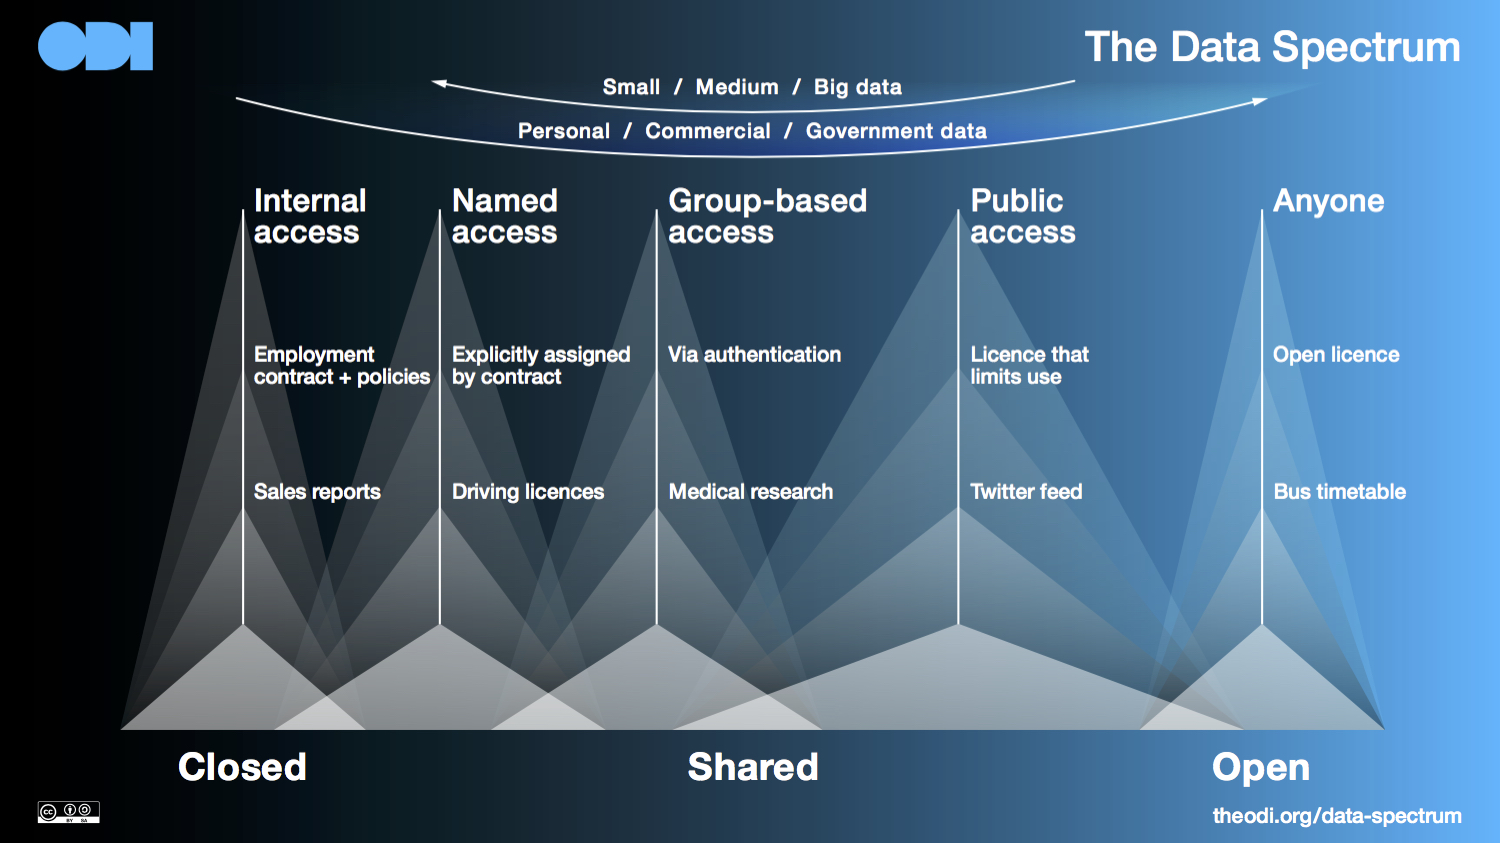
\includegraphics[scale=0.3]{images/odi_open_data_spectrum.jpg}
\caption[Data Spectrum as a definition of steps between open and closed data.]{Data Spectrum as a definition of steps between open and closed data. Source: \url{https://theodi.org/data-spectrum}}
\label{fig:data_spectrum}
\end{center}
\end{figure*}

With the same idea of defining intermediate levels of data openness, \citeonline{Bargh2016} proposed the Semi Open-Data Paradigm.
The objective is the analyse the dissemination of data through several dimensions, as publicity, completeness, timeliness, metadata, and other.
For each dimension, several level should be defined.
On the publicity dimension, the proposed levels are: ‘share with no one’, ‘share data within a specific group’, ‘share data within a department of an organization’, ‘share data within an organization /ministry’, and ‘share data among a federation of organizations’ and finally ‘share with the public’.

%######################################################################
\section{Open Data Landscape}
\label{sec:opendatalandscape}

While the number of open data initiatives around the world increases dramatically every year, several research projects driven from academy and/or civil society organizations seek to map the open data landscape.
In the following, some of these projects are summarized, and their main results are presented:

\textbf{\href{http://index.okfn.org/}{Open Data Index}:} The Open Data Index is one of the most important platform for analysing the open data landscape in the world. In 2013, the first year, Open Data Index analysed 60 countries. In 2014 this number grew to 97, and in 2015 the evaluation covered 122 countries.
The methodology consists basically in analysing datasets from 13 categories: 
National Statistics, Government Budget, Legislation, Procurement tenders, Election Results, National Map, Weather forecast, Pollutant Emissions, Company Register, Location datasets, Water Quality, Land Ownership and Government Spending.
For each category, 9 features are evaluated with yes or no answers: ``Openly licensed?'', ``Is the data machine readable?'', ``Is the data available for free'',  ``Available in bulk?'', ``Is the data provided on a timely and up to date basis?'', ``Is the data available online?'', ``Is data in digital form?'', ``Publicly available?'' and ``Does the data exist?''.
From this analysis, a ranking is constituted according to each countries \emph{score}. 
This score is a weighted sum that reflects the performance of each category for each feature.
Considering all the countries, only 9\% of the datasets are open. 
However, a strong inequality between the countries can be seen: while 25 of them have 50\% or more datasets open, 44 have less than 25\%.

\textbf{\href{http://www.opendatabarometer.org/}{Open Data Barometer}:} The Open Data Barometer also focus on a comparison of the open data context between countries. However, a more complex methodology is used to analyse each country, including expert interviews and secondary data, apart from accessing the datasets in a similar way as the Open Data Index.
The 2nd Edition of this research, released in January 2015, analysed 86 countries concluded that ``there is still a long way to go to put the power of data in the hands of citizens''\cite{Davies2015} .

\textbf{\href{http://opendatamonitor.eu/}{Open Data Monitor}:} The Open Data Monitor is focused on looking at datasets from European countries. One interesting aspect of this project is the measurement of ``availability'', which considers the existence of ``a description, at least one resource with a functional link and an available email of the author'' for datasets in a catalogue.
Surprisingly, the first three countries with more datasets (Germany, UK and Spain) have only a bit more than half of their datasets available (51\%, 63\%, 57\%, respectively).

\textbf{\href{http://opendatainception.io/}{Open Data Inception}:} This project presents the largest geotagged listing of open data portals, with more than 1600 ODPs showed in a map. For each portal, URL and associated geographical region is given.

\textbf{\href{http://right2info.org}{Right2Info}:} This platform monitors FOIAs, which is not specifically open data, but is very related. 93 countries have some kind of FOIA, and the platform presents a comprehensive list of 273 FOIAs covering various scopes~\cite{Vleugels2012}.

\section{Open Budget Data}
\label{sec:openbudget}

From all types of OGD, one is of particular importance: government budgetary data, as timely access to these data is critical to accomplish government accountability.

All governments and public administrations maintain budgetary data, unlike, for example, bus position data, which depends on sensors, or data about the occurrence of a specific disease, which depends on a health information system.
From the citizen side, information on budget is a key element to ensure that public funds are being properly used.
In locations where a participatory budget~\cite{Mkude2014} was implemented, that is, part of the budget allocation is decided by the community, access to this kind of data is indispensable.
A global initiative to improve openness of governments -- the Open Government Partnership (OGP) -- has the fiscal transparency as minimum eligibility criteria\footnote{Other criteria can be found at \url{http://bit.ly/1929F1l}.}, characterizing budget data as a foundation of open government.


%%openbudget eu * edited
Even with so many possible positive impacts, existing public financial transparency portals suffer from a number of shortcomings.
First of all, they suffer from the large number of diverse data structures that make the comparison and aggregate analysis of transnational financial flows practically impossible. 
The tools to present, search, download and visualise this financial data are also nearly as diverse as the number of existing portals. 
This heterogeneity may even prevent an analysis of the quality of the data for the same funds administered by different funding authorities~\cite{Vafopoulos2013}. 
Past efforts have sought to overcome this situation by creating comprehensive and connected transparency portals, such as Farmsubsidy.org, and more recently, Publicspending.net.
%However, the diversity of transparency standards across Europe, which proved to be a bottleneck, highlighted the need that platforms beyond the state-of-the-art also need to be more than just direct entry points to financial data analysis.
%They also need to provide a platform for advocacy towards common transparency standards at the highest level across several jurisdictions.
%%
Within the existing open budget initiatives, low user engagement has been reported~\cite{Worthy2013}. 
Moreover, most of the budget publishing efforts results in simple data catalogues, fragmented and dispersed, because they do not share standards and methodologies~\cite{Vafopoulos2013}. 
The absence of standards can lead to data misuse~\cite{Zuiderwijk2014a}, or even to results opposed to the initial aims~\cite{Gurstein2011}.

In~\citeonline{Tygel2016}, we proposed a \emph{structured analysis framework} in order to explicitate problems generated by the lack of standards and help policy makers to understand the importance of various aspects of budget data publishing. We also envision the framework as a tool to design more adequate budget publishing systems. Together with other ongoing initiatives~\cite{OpenSpending,Vlasov2014}, we believe that the development of a solid standard can help governments to make their budget data more usable, and thus enable citizen participation in the democratic process. The framework can be seen in \autoref{fig:framework}.

\begin{figure*}[ht]
\begin{center}
%\includegraphics[scale=0.50]{Images/framework.png}
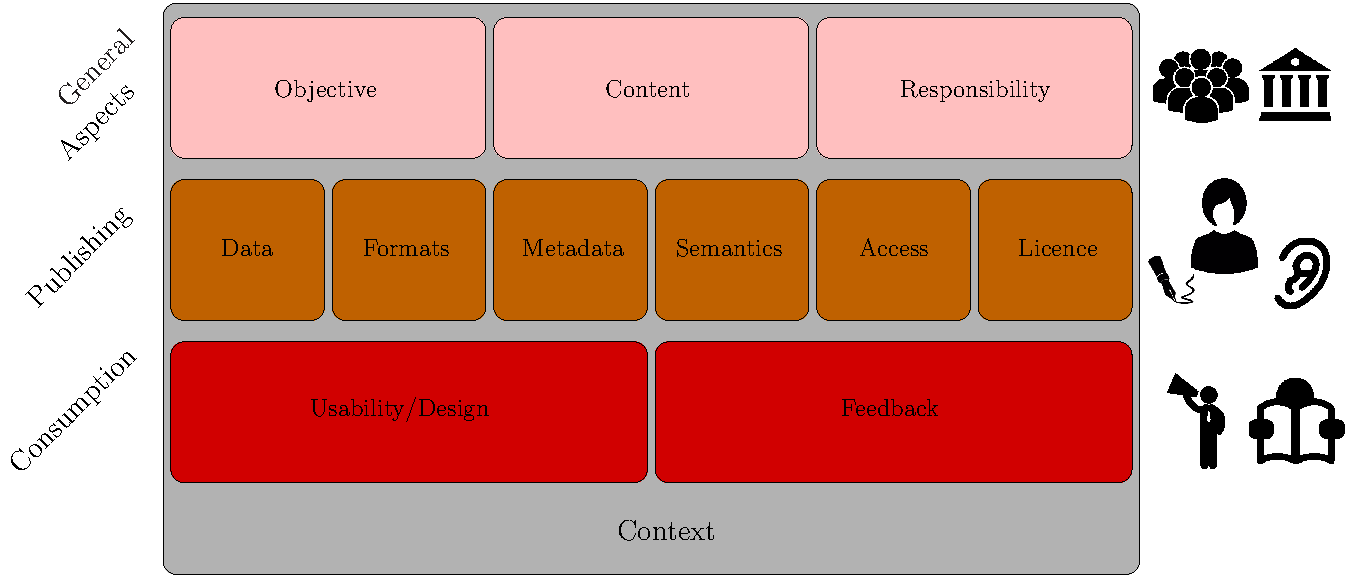
\includegraphics[scale=0.75]{images/model.pdf}
\caption[Analysis framework open budget initiatives.]{Analysis framework for open budget initiatives. The four parts -- General Aspects, Publishing, Consumption and Context -- are interconnected, and composed by several dimensions. Icons:\href{http://www.flaticon.com/authors/icomoon}{Flaticon (CC)}.}
\label{fig:framework}
\end{center}
\end{figure*}


Results from the application of this framework to 23 open budget initiatives can be seen at \url{http://bit.ly/1FNThhH}.
The goal of the evaluation is not to be extensive or to achieve statistical significance, but rather to test the model, to discover its potentials and limitations, and to gain some intuition on the domain.

The 23 initiatives were chosen considering a balance between primary (11) and secondary (12) sources. 
The sample also contains at least five initiatives strongly related to each use perspective, and considers initiatives from 6 countries plus the European Union, presented in five different idioms. Some of the analysed initiatives are listed on the \emph{Map of Spending Projects}\footnote{Available at \url{http://community.openspending.org/map-of-spending-projects/}.}.

All primary sources are maintained by the government, and most of the secondary ones are society driven. 
Among them, two initiatives were identified as maintained in partnership between government and society organizations. 
Initiatives generally display their objectives (22), but only 11 explicitly mention their intended audience. 
Also, almost all initiatives offer data for download (18), which favours transparency perspective, and more than half of them (13) make visualization available, favouring participation perspective.

Even considering the low number of initiatives evaluated, two outcomes drew the attention, regarding feedback and semantics. 
Commenting on data is allowed only in three initiatives, and the same number (but not the same ones) offers a data request form.
No reporting issues mechanisms were found, revealing a strong absence of feedback possibilities.

The lack of semantics support (only three offered it), or linkable data (again, only three had it) also may point that policy marking perspective is still far from reality. 
Ten initiatives use categories for the datasets, which at least facilitate some form of comparisons.
Regarding the use perspectives, we can state:

\noindent\textbf{Transparency:}
The main requirements for this use perspective -- data on transaction level, machine readable formats and aggregation levels -- were accomplished by most of the open budget initiatives. 
However, much work is still to be done concerning the feedback handling.
We can say that, for most of the analysed cases, stakeholders interested in auditing government and in translating data into more accessible formats are partially satisfied.

\vspace{.1cm}

\noindent \textbf{Participation:}
The requirements set for this use perspective enforced human readable formats that allow citizens without deep budget knowledge to understand data and to participate in discussions.
Slightly more than half of the initiatives present graphics, which can help quick insights over data.
Only three initiatives offer maps to visualize budget data, what is coherent to the low number of initiatives that include the location dimension (eight).
Another aspect emphasized in this use perspective was the usability and design. 
Considering the already mentioned limitations on assessing this issue, we noticed that ten initiatives use standard open source software tools. 
Although this is not the most relevant factor regarding usability, the use of standard tools favours users dealing with several open budget initiatives.
Moreover, as open source tools, the more initiatives using these tools, the better they can be developed.

\vspace{.1cm}

\noindent \textbf{Policy Making:}
The main requirements in this perspective were the use of common classifications, vocabularies and ontologies, and the possibility of linking data with other databases.
As already mentioned, semantics support was mostly absent. Comparison tools, also important in this case, were found only in three of the initiatives. 
Thus, this use perspective is still far from being realised in most of the analysed initiatives. 
All these indicate that working on standard terminologies and common conceptualizations as suggested by OpenSpending~\cite{OpenSpending} is highly desirable.

The application of the model to 23 open budget initiatives made possible to derive several conclusions related to the specific use cases.
However, it would be necessary a larger number of analysis and more iterations of the inductive-deductive approach in order be sure about the completeness of the model.

\section{Evaluating Open Data Impacts}
\label{sec:impacts}

Although mapping initiatives is a very important way of assessing the quality of published data between countries, very little is known about the final effects of these policies.
Almost a decade after the implementation in large scale of open data policies, researchers and practitioners start to pose the question: how to assess open data impacts on the society?

In order to tackle this question, a theoretical background to analyse the impact of OGD was developed by~\citeonline{Granickas2013}. 
Impacts are divided into economic, political and social, and for each of them, possible implementation issues and impact metrics are deeply discussed.
Recently, a working group was created to develop methods for assessing open data. In their first report~\cite{Caplan2014}, a draft of a framework is proposed.

Finally, a recent report run a thorough review over evidences of impacts of fiscal openness~\cite{Renzio2015}. While recognizing that there is a literature gap on testing causal effects, the most rigorous studies found a relation between open budget initiatives and the desired outcomes.

An impact evaluation and comparison between almost 30 Brazilian government transparency portals, on several administration levels, is presented by~\citeonline{Beghin2014}. The analysis was based on the 8 Open Government Principles evaluated for each portal by experts. Despite being a well defined and wide accepted model, these principles are quite general, and do not refer to specific characteristics of budget data. Moreover, they cover basically the publisher side.


\section{Open Data Value}
\label{sec:value}

Another way of assessing open data impacts is through the analysis of \emph{open data value}.
Releasing social and commercial value is cited under the main motivations for governments to publish open data (see \autoref{sec:why}).
Thus, it is necessary to understand the chain of value addition over data, and specifically what activities may add value for data.
\citeonline{Jetzek2013} developed a conceptual model of OGD value generation, where enabling factors lead to value generation mechanisms which should finally release social and commercial value. 

\citeonline{Attard2016} proposed a Value Creation Assessment Framework, which profits from previous works, and extends some aspects.
The framework walks through the complete Government Data Life Cycle Processes, namely: data creation, harmonisation, publishing, interlinking, exploitation and curation, and defines implementation and impact aspects related to each stage.

%\section{Open Data and Participation}

%Enabling citizen participation in democracy is one of the mentioned motivations for using open data.
%The reasoning behind it is that the release of open data makes citizens more informed, and thus are more able to participate in public decisions.
%One of the most famous processes of citizen participation is the Participatory Budget.

%\begin{itemize}
%	\item Origins of PB, and impact analysis in Brazil~\cite{Goncalves2014}
%	\item Definitions: \cite{Zhang2013}
%	\item Description of Cuiabá case: \cite{Borges2012}
%	\item PB critics: \cite{Masser2013}
%	\item 10 reasons to implement: \cite{Nitschke2013}
%	\item Comparisson between online and offline PB: \cite{Peixoto2009}
%	\item Conditions for participation: \cite{Addor2012}
%	\item Budget data publishing process, including feedback: \cite{Alexopoulos2014}
%	\item Deep analysis about PB, focusing on the poor \cite{TheWorldBank2001}
%	\item Literature review, definitions and a model to analyse PB \cite{Miller2014}
%\end{itemize}

%As a complementary approach, we also interviewed two domain experts: 
%\begin{itemize}
%	\item a government employee who activeley supported a PB process
%	\item and the director of a transparency oriented Civil Society Organization (CSO)
%\end{itemize}


%%
%#############################################
\subsection{Introduction}
%#############################################
The literature about participatory budget is vast. The possibility of enhancing democracy through direct participation of citizens in a crucial political decision, i.e., budget allocation, attracted the attention of researches since the first well known experiences in Porto Alegre, in the 1980 decade.

Since then, several implementations all over the world were experimented, with many successful and fail stories. The use of online tools, both for supporting PB process and for publishing related datasets was also part of the more recent experiences.

In this review, we try to picture the state of art of PB, pros and cons and the mechanisms used, with a special focus on the online ones. The final objective is to detect how online information systems can help build a more effective participation, both higher and better informed, to produce better outcomes.

%#############################################
\subsection{Summary of Analysed of Works}
%#############################################
\begin{itemize}
	\item Origins of PB, and impact analysis in Brazil~\cite{Goncalves2014}
	\item Definitions: \cite{Zhang2013}
	\item Description of Cuiabá case: \cite{Borges2012}
	\item PB critics: \cite{Masser2013}
	\item 10 reasons to implement: \cite{Nitschke2013}
	\item Comparisson between online and offline PB: \cite{Peixoto2009}
	\item Conditions for participation: \cite{Addor2012}
	\item Budget data publishing process, including feedback: \cite{Alexopoulos2014}
	\item Deep analysis about PB, focusing on the poor \cite{TheWorldBank2001}
	\item Literature review, definitions and a model to analyse PB \cite{Miller2014}
\end{itemize}

As a complementary approach, we also interviewed two domain experts: 
\begin{itemize}
	\item a government employee who activeley supported a PB process
	\item and the director of a transparency oriented Civil Society Organization (CSO)
\end{itemize}

%#############################################
\subsection{Origins}
%#############################################

\cite{Goncalves2014} describes the first PB experiences in Brazil in the context of the country's redemocratization. After 20 years of military dictatorship, in the late 1980's, many efforts were driven in order to decentralize the public administration, from the federal level to the cities. In this context, the Workers Party was created, and as soon it elected the first mayors, PB was implemented as a symbol of direct democracy and transparency, as oposed to the previous regime.

Still according to \cite{Goncalves2014}, in Porto Alegre, the most cited PB showcase, the number of participants raised from around 1000, in 1989, to around 20,000 in the late 1990/early 2000. The alleged reason is that the people demands were realy undertaken by the governments.

According to \cite{Miller2014}, in 2010 nearly 1,500 municipalities worldwide adopted PB.

%#############################################
\subsection{PB Cycle}
%#############################################
According to~\cite{Giacomoni2007}, the classical Budget cycle comprises 4 phases:

\begin{enumerate}
\item Elaboration and presentation
\item Legislative authorization
\item Programming and execution
\item Evaluation and controll;
\end{enumerate}


Figure~\ref{fig:POA} shows the workflow used in Porto Alegre.

\begin{figure}[h]
\begin{center}
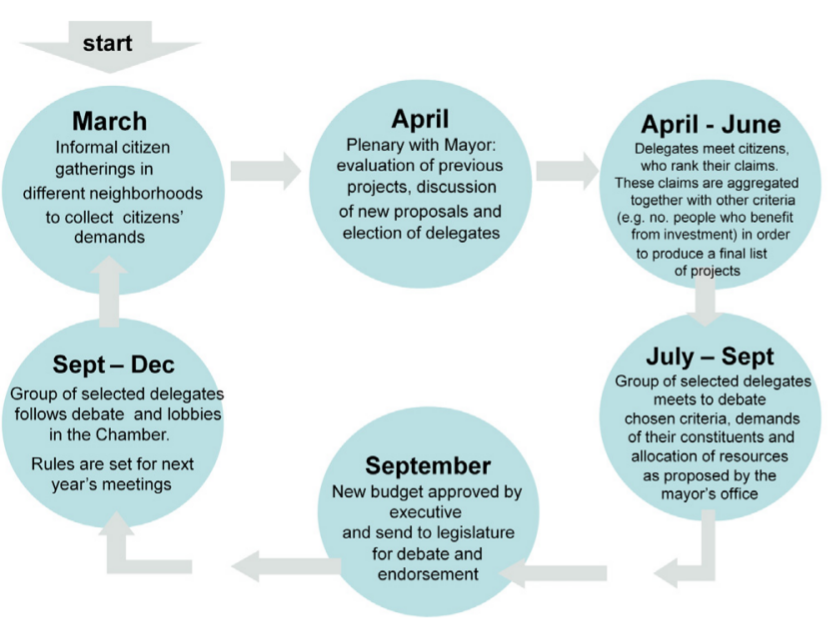
\includegraphics[scale=0.35]{images/portoalegreworkflow.png}
\caption{Workflow of Porto Alegre's PB. Author: \cite{Goncalves2014}\label{fig:POA}}
\end{center}
\end{figure}

\cite{TheWorldBank2001} summarizes four fases, illustrated in Figure~\ref{fig:WB}:
\begin{enumerate}
\item Budget formulation
\item Budge analysis
\item Budget expenditure
\item Performance monitoring
\end{enumerate}

\begin{figure}[h]
\begin{center}
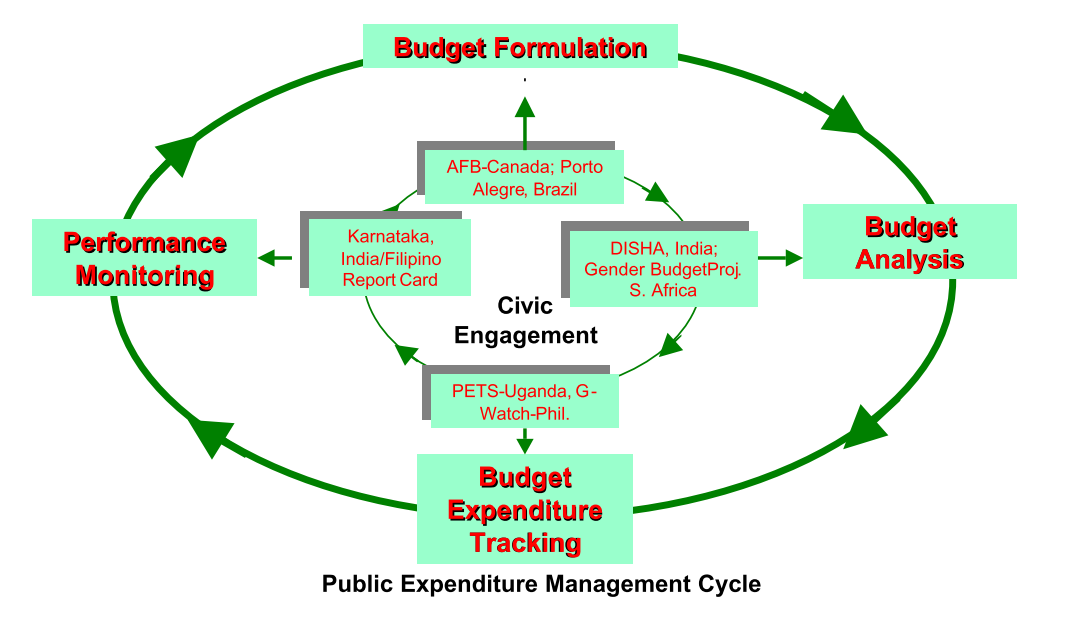
\includegraphics[scale=0.35]{images/cycle_WB.png}
\caption{Generic PB Workflow. Author: \cite{TheWorldBank2001}\label{fig:WB}}
\end{center}
\end{figure}



%#############################################
\subsection{Definitions}
%#############################################

\cite{Zhang2013} proposed some definitions on this field:

\noindent\textbf{Participatory budgeting} refers to a situation in which government officials invite citizens' input during the budget process and allows citizen to influence budgetary decisions (Zhang \& Yang, 2009).

\noindent\textbf{Mechanisms of participatory budgeting} refer to any tools provided by government for citizen involvement, including public hearings, citizen surveys, telephone hotlines, citizen advisory boards, focus group, as well as encouraging citizens to speak about budget in regular meetings, posting budget materials on the Internet, working with local media to highlight citizen comments during deliberation, and so on.

These mechanisms are of two kind:

\noindent\textbf{One way mechanisms:} Coordinating with the local media, such as TV and radio, to invite the public comments; Citizen surveys about spending priorities and needs through mail, Internet or telephone; Posting budget materials on Internet sites; Hotlines for citizens to provide suggestions or comments.

\noindent\textbf{Two way mechanisms:} Public budgetary hearings; Forums or workshops open to citizens during budget preparation; Opportunities for citizens to speak at regular meetings; Citizen advisory boards; Focus groups.
We define “two-way communication” as a process of face-to-face interaction between citizens and government officials in which citizens are provided with an opportunity to directly raise concerns and discuss them with government officials. Two-way communication can nurture social learning and collaborations between citizens and government because it enables stakeholders to respect and listen to one another’s opinions, and allows competing perspectives to be aired and considered before decisions are made (King, Feltey, \& Susel, 1998; Roberts, 2004).

In his review, \cite{Miller2014} also collected a number of other definitions. They also point some literature confusions, specially in the US. One of the points is that labelling the above mentioned one way mechanisms as PB ``eliminates from participatory budgeting what is distinctive, valuable, and potentially transformative".

%#############################################
\subsection{Motivations for implementing PB}
%#############################################

In a sort of ``marketing paper", \cite{Nitschke2013} proposes 10 reasons for public administrations to addopt PB:

\begin{enumerate}
\item Greater acceptance of priorities that are better harmonised
\item Making administration more efficient by integrating citizens’ knowledge
\item Increasing problem-solving capabilities
\item Greater cost awareness
\item Mobilising citizen engagement
\item Reducing political disenchantment and disillusionment with political parties
\item Fostering democracy
\item Supporting modernisation processes within the administration
\item Improved image for the local authority
\item Risks do exist, but they can be successfully managed
\end{enumerate}

As we will see in the next section, many of these ``benefits" can turn into impediments if not well implemented.

The political conditions for a sucessfull participation process are object of a political science oriented study by \cite{Addor2012}. After deeply analysing two experiences - not only of PB, but of wider participation practices - he formulated seven factors that influenced on the establishment and strengthening of the participator practices:

\begin{enumerate}
\item Politicisation of the society
\item Transformation of the reality
\item Permission of the utopia
\item Basis organization
\item Exchanges with other experiences
\item Involvement of the state
\item Formalization of the political commitment
\end{enumerate}

%#############################################
\subsection{Criticisms on PB}
%#############################################

\citeonline{Masser2013} summarized common criticisms to PB, specially in the German context. He considered that the first wave of PB experiences in the country failled: ``The original objective of involving citizens in the complex process of municipal budget formulation was not achieved, and has since been abandoned. Nowadays, it is only collections of proposals for measures and (investment) projects, or voting procedures on proposals made by policymakers and administrators, that operate under the label ‘participatory budgeting’."

The first argument is about \textbf{low participation}. ``The question therefore arises of whether the measures identified through PB possess sufficient legitimacy to warrant their adoption by democratically elected local councils."

This leads to a second argument that states the \textbf{under representation} of the society in PB practice.

Another argument lies in the \textbf{high cost of participation}, which is a consequence of the low participation. ``The low figures for participation raise another problem:  how sustainable is citizen participation through PB? In many cases we can see that PB has already been discontinued. The question as to whether ‘participatory budgeting’ as a whole is gradually fading away seems warranted. This is because, as with employee suggestion schemes, in PB fresh ideas are not forthcoming every day. In fact, there is a risk that the debate will keep returning to many similar proposals or even the same ones."

\textbf{Conclusions:}
The original intention of integrating citizens closely into the budget formulation process has not been realised;

The influence that citizens wield in this procedure is limited, because only a few proposals made by a few citizens have a chance of being realised, even though each and every citizen does have an opportunity to influence things by prioritising and voting on the proposals;

The fact that the influence of citizens is not all that significant might also benefit PB, in that members of local councils might then be far more willing to embrace this tool. 

There remains a trend toward PB. The Fifth Status Report on ‘Participatory Budgeting in Germany’ published in March 2012 identifies 21 newly active municipalities that are conducting PB. This makes a total of 115 active local authorities that are either conducting PB or have at least done so within the last two years.

%#############################################
\subsection{Some current PB cases}
%#############################################

\subsubsection{\href{http://pbnyc.org/}{New York}}
``New York City is experiencing a new kind of democracy. Through Participatory Budgeting, residents of twenty-four Council Districts across the City are directly deciding how to spend \$25 million of taxpayer money. From September 2014 to April 2015, community members are exchanging ideas, working together to turn ideas into project proposals, and voting to decide what proposals get funded."

\subsubsection{\href{http://cambridgema.nationbuilder.com}{Cambridge}}
``In December, community members shared over 380 ideas for projects to improve Cambridge.  From January-March, 40+ volunteer Budget Delegates prioritized and developed those ideas into 20 concrete project proposals for community members to vote on. Over 2,700 Cambridge residents age 12 and older voted online and at events around town from March 22-28, 2015 to decide which projects the City should fund."

\subsubsection{\href{https://budgetparticipatif.paris.fr}{Paris}}
In Paris, the major selected 15 projects and made \$20 million Euros for that. Over 40,000 people participated, being 40\% online. Among the 15, nine project were chosen to be developed in 2015. This year, almost 20,000 people proposed over 5,000 ideas.

\subsubsection{\href{http://planejasampa.prefeitura.sp.gov.br/}{São Paulo}}
In São Paulo, the Planning and Budget Participatory Cycle envisages a four year cycle, and is based on fisical goals. Direct participation resulted in 123 goals. 11,000 people formulated (physically) 9,489 suggestions, which resulted in the goals. There were also 2 hacker meetings, with 100 presential participants. A tool was developed for monitoring the goals by the elected councillors.

\subsubsection{Other related links}
\begin{itemize}
	\item \href{http://pbnetwork.org.uk/}{PB Network (UK)}
\end{itemize}

%#############################################
\subsection{Profile of the Participants}
%#############################################
\cite{Masser2013} reports that ``The vast majority are middle-aged men who left school well-qualified and now have well-paid jobs". 

On the other hand, \cite{Goncalves2014} reports that ``data collected at the participatory budgeting forums in Porto Alegre, in 2002, reveal that the participatory assemblies tend to concentrate a higher proportion of (i) women, (ii) elders and retired workers, (iii) married people, (iv) non-qualified workers, (v) people with lower average income, (vi) higher rates of associative life, and (vii) stronger identification with the Workers’ Party ideology than the city’s average dweller."

\cite{Peixoto2009} also reports advanced age and lower socio-economic background.


%#############################################
\subsection{The role of online tools in PB}
%#############################################
The use of online tools for PB was described by \cite{Peixoto2009}. According to him, ``evidence suggests that the online forum was, overall, an environment of rational, argumentative and reflective debates where active participants would persuade and be persuaded of the importance of one public work over another and where readers - in larger numbers - could be informed on concurrent perspectives."

In the voting for priorities, as expected, the participation was higher than the standard PB. It was noticed that people tend to vote locally, i.e., to choose works near their residences. This is also somehow expected, as the original target of PB is to descentralize power and let communities decide what is better for them.

``One element that was considered important for the success of the e-PB was the city’s communication campaign, which focused on the initiative and its novelty factor.''

Finally, the author considers that online PB should be just a complementary action to be taken together with tradiciontal PB. 


%#############################################
\subsection{Linking Budget Planning with final result}
%#############################################
As pointed by several works \cite{Addor2012, Miller2014, TheWorldBank2001, Borges2012}, a crucial element for raising participation is to guarantee that the decisions taken by the citizen council will be really implemented. Although this is a quite obvious conclusion, the disconnection between what is decided and what is implemented has been pointed to be the reason of several PB experiences (\cite{Borges2012}).

One of the interviewees was a government employee responsible for coordinating a PB process in a medium size city in Brazil. The process of collecting citizen demands was successful, with high participation of citizens and community leaders. All PB assemblies had the presence of at least four government representatives, so that proposals could be discussed with the ones responsible to implement it. 

However, the final result was modified by the legislative, and not totally implemented in the following year. In second year of PB, a new mayor was elected, and PB received less attention. The government officials stopped attending the meeting, and PB failed.

Another big issue pointed by the interviewee was the lack of transparency inside government. In his opinion, government information systems suffer from a lack of integration that seriously compromises transparency. With an integrated information approach, citizens could easily follow a demand from budget planning until the execution, and even assess specific targets, for example, more kids on the school or decrease of illness caused by lack of sewage.

The second interviewee, member of a transparency oriented SCO, reported the same scenario of decoupled systems in another medium size city in Brazil, which deeply hinders transparence. A mayor change altered positively the scenario, but crucial measures, as online procurements, were still no implemented. He calls the attention also for a transparency in the councils, because many times, council members may be representing private interests, or not representing anything at all.

One aspect point by this domain expert is the financing of participation. He pointed that, many times, counting only on voluntary efforts may not be enough to audit the government. On the other hand, possible financiers, as commercial association, may have different interests in relation to transparency.



%#############################################
\subsection{Open Budget Experiences}
%#############################################

In the specific field Open Budgets, the experience of three countries was recently reported: \href{http://fiscaltransparency.net/wp-content/uploads/2015/03/GIFT-Kenya-Webinar-Deck.pdf}{Kenya}, \href{http://fiscaltransparency.net/wp-content/uploads/2015/03/GIFT-MEX-TP-Webinar-Deck.pdf}{Mexico} and \href{http://fiscaltransparency.net/wp-content/uploads/2015/03/GIFT-Chicago-NYC-Webinar-Deck.pdf}{Chicago and NYC}.

A \href{http://pt.slideshare.net/jwyg/open-budget-data-a-landscape-analysis}{landscape analysis} with several definitions and cases was also presented.

%#############################################
\subsection{Software Tools}
%#############################################

\noindent\textbf{\href{http://budgetallocator.com/}{Budget Allocator}: } This online tools is a one way mechanism of budget participation. It offers the citizen the chance to submit a number of choices - increase, decrease or maintain police expends, for example, or build a pool, a school or a hospital - and some comments over it. If your choices are over budget, the system warns about a possible tax increase. The licence costs between U\$200 and U\$2000.

\noindent\textbf{\href{http://www.engagedata.eu/}{Engage}: } With this platform, users are able to submit, acquire, search and visualize diverse, distributed and derived Public sector datasets from all the countries of the European Union. A special focus is given on the feedback loop. The tool allows discussion and suggestions on specific datasets, as described in~\cite{Alexopoulos2014}.

\noindent\textbf{\href{https://www.participare.io/}{Participare}: } `` It provides an easy to use, do-it-yourself like, Participatory Budgeting platform capable of adapting to the best practices as well as local specificities."

\noindent\textbf{\href{https://docs.google.com/spreadsheets/d/1f1iHQFGIc5MmmzdRVkBk6hXyrrLnoNP4aaOM9w85agw/}{OpenSpending List}: } List of 60 softwares which support some kind of participation.

%#############################################
\subsection{Some conclusions}
%#############################################
\begin{itemize}
\item Participatory budget is, most of all, a political action. The only possibility for it to work properly is to be fully and truly supported by the government;
\item Given the political support, it is also important to 'close the loop', i.e., connect the ellected demands with the monitoring of the concrete results and the high level targets;
\item Online tools have to be combined with presential strategies, and must cover the whole budget cycle - from definition to target monitoring.
\end{itemize}



\section{Problems of Open Data}
\label{sec:problems}

The vast majority of research about open data assumes that publishing public data in open formats will bring mostly good impacts.
In this sense, two works from the same research group made an in depth research on the negative sides of open data.

In the first one, \citeonline{Zuiderwijk2012} analysed the socio-technical impediments that hinders the use of open data via literature review, interviews and workshops.
As a result, 118 impediments were summarized in 10 categories: availability and access, find ability, usability, understand ability, quality, linking and combining data, comparability and compatibility, metadata, interaction with data provider and opening and uploading.

The second paper focuses on the possible negative effects that governments may face on opening data. \citeonline{Zuiderwijk2014a} conducted several interviews with public servants and data archivists to find out which negatives effect they were concerned with.
As a result, 16 negative effects were listed, for example: ``risk of violating legislation by opening data'', ``privacy can be violated unintentionally'', ``misinterpretation and misuse'', ``not citizens but others profit from open data'' and ``wasting resources to publish invaluable data''.
It is interesting to note the question of data value also appearing here.
In fact, methods for determining the value of data for users could help publishers selecting in which data should they put efforts.

Regarding the risk of privacy violation, two recent episodes attest that these concerns should really be taken into account.
As reported by \citeonline{Hern2014}, the opening of taxi trips data by the city of New York allowed the identity of drivers to be discovered, and in some cases, even the passengers could be identified.
In a similar situation, the release of film ranking data allowed not only the identity of users to be unveiled, but also their political orientation, religious views or sexual orientation.
In both cases, the attempt to anonymise data failed.

\citeonline{Parycek2016} interviewed public servants in German speaking regions in order to gather barriers for the implementation of open data in the public sector.
As result, three main impediment classes were found: information cultures and divergent interests in agencies, limited innovation potential in organizational cultures and limited communication of strategies.
Authors conclude that ``if organizational aspects of information culture are not addressed, the value of Open Government might not be understood'' and that ``cultural and organizational factors, as opposed to a simple lack of knowledge, play a crucial role regarding the implementation of open technologies in the German-speaking region.'' \cite[p.7]{Parycek2016}.

\subsection{The Missing Focus on Use of Open Data}

Another aspect revealed by~\citeonline{Zuiderwijk2014a} is the lack of informations interest about the actual use of open data: ``The interviewees stated that they do not have much more information about how the open data have been used than the number of downloads''.

One of the few works dealing with this subject was written by~\citeonline{Davies2012}. According to the author, ``The gap between the promise and reality of OGD re--use cannot be addressed by technological solutions alone''.
Thus, he raises the necessity of considering human factors that affect the use or no use of data.
In this paper, a Charter of Open Data Engagement is proposed, aiming to derive a parallel of the Five Stars of Open Data~\cite{Berners-Lee2010}, but from the users point of view.

The five stars of open data engagement are~\cite{Davies2012}:

\begin{itemize}
	\item Be demand driven;
	\item Put data in context;
	\item Support conversation around data;
	\item Build capacities, skills and networks; and
	\item Collaborate on data as a common resource.
\end{itemize}

In the same work, Davies criticizes the so called ``application fallacy''.
According to him, the narratives about OGD assume that someone will develop an application to consume and visualize data.
However, in his master thesis,~\citeonline{Davies2010} ran a survey with 55 instances using OGD from data.gov.uk, which revealed that in most of the cases facts are directly identified within datasets.
Data is then used to base discursive reports, or to generate derivative datasets.

\citeonline{Davies2010} describes five ways of using open data. 
\autoref{fig:opendatause} shows the categories, and the number of cases gathered on the survey.

\begin{figure}[h!]
\begin{center}
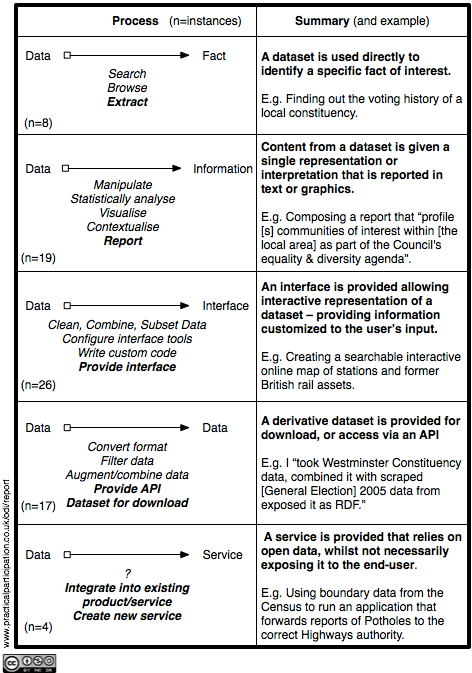
\includegraphics[scale=0.6]{images/Data-Schematic-FiveTypes}
\caption[Different uses of data, with process, summary and examples.]{Different uses of data, with process, summary and examples. For each type, the number of instances (n) found is detailed. Source: \citeonline{Davies2010}}
\label{fig:opendatause}
\end{center}
\end{figure}

As a contribution for future research, author cites some challenges in the social and technical fields.
The priority, according to him, is to understand the process that occurs between data publishing and its use in a determined application.
Through this understanding it will be possible to overcome the barriers for use of data.
Moreover, it is necessary to explore the existent political structures, so that the informations brought by data can effectively generate social changes.
Finally, the broader challenge is to better understand the user point of view.
The greatest technical challenge associated is to create tools that not only show data, but that support discussion and interaction around them.

\subsection{Open Data Capacities and Data Divide}
\label{sec:datadivide}

Still according to~\citeonline{Zuiderwijk2012}, two of the broad categories of open data impediments are ``Usability'' and ``Understand ability'', under which 33 problems were mapped.
Under these, we can list at least seven directly related to the lack of capacities from the user side deal with data:

\begin{itemize}
	\item Data are not understandable for the general public (e.g. related to jargon). 
	\item No explanation of the meaning of data. 
	\item Lack of knowledge about how to interpret the data. 
	\item Lack of skills and capabilities to use the data. 
	\item Lack of statistical knowledge.
	\item Lack of (domain) knowledge about how to treat the data. 
	\item Expert advice is needed to use the data.
\end{itemize}

\citeonline{Zuiderwijk2014a}, based on several interviews with government officials, affirm that this lack of capacities in using data may lead to negative effects in open data: 

\begin{citacao}
(...) stakeholders do not profit equally from the opening of data. The use of open data is complex, time-intensive and might require certain skills to find, understand and use data. This results in a high threshold for ordinary citizens to make use of the data. Instead journalist and lobbyist have more time and are often skilled in making use of the data. As such open data can be used by certain groups to strengthen their position, instead of creating a level playing field~\cite[p.150]{Zuiderwijk2014a}.
\end{citacao}

Inequalities in access to data is starting to raise concerns for those who, for many years, studied the inequalities in access to ICTs.
Micheal Gurstein is probably the pioneer in calling attention for this and coining the term \emph{data divide}: 

\begin{citacao}
Efforts to extend access to “data” will perhaps inevitably create a “data divide” parallel to the oft–discussed “digital divide” between those who have access to data which could have significance in their daily lives and those who don’t \cite[p.2]{Gurstein2011}.
\end{citacao}

A data divide between countries is also mentioned as one of the conclusion of the Open Data Barometer project.
\citeonline{Davies2015} states that the data divide between countries has grown from the first edition of the evaluation, in 2013, to the second one, in 2014.
Countries are clustered into four classes to define their stage in implementing open data policies: High capacity, Emerging and advancing, Capacity constrained and One sided initiative.

Another important publication which shows concerns with data divide is the report by the~\citeonline{DataRevolutionGroup2014}: ``There are huge and growing inequalities in access to data and information and in the ability to use it''.
The group hosted by the United Nations warns that ``Without immediate action, gaps between developed and developing countries, between information-rich and information-poor people, and between the private and public sectors will widen, and risks of harm and abuses of human rights will grow.''

\subsection{Organization Challenge}
\label{sec:org_problem}

In order to be usable, published open datasets have to be organized in a logical way that allows people to find it.
Regarding open data repositories, the organization challenge has an internal aspect, i.e., the way each ODP organizes their own data, but also a global aspect, regarding to a harmonization among different repositories.
Both issue are directly related to the proper use of metadata.

The impediments compilation by \citeonline{Zuiderwijk2012} cites some related problems, such 
as ``absence of commonly agreed metadata'', ``insufficiency of metadata'', ``the lack of interoperability'' and ``difficulty in searching and browsing data''.
The same study also states that ``A lack of open data standards between (levels of) government organizations has been identified as a barrier to open data usage by citizens and businesses and subsequently new open data policy''.

When analysing open data of different contexts, language aspects quickly emerge: ``Language barriers and interoperability aspects need to be tackled so that information resources from different organizations and countries can be combined'' \cite{Zuiderwijk2012}.

Organization is also problem for agents in the private sector willing to use open government data.
According to~\citeonline{Roseira2016}, firm managers interviewed point out that most datasets have incomplete or nonexistent metadata.
This lack of data quality generates a higher workload on cleaning and harmonizing data.
The study included that firm managers desire to see advances on datasets standardization in order to boost open data economic value creation at national and international levels.

\section{Linked Data towards Semantic Organization of Open Data}
\label{sec:LOD}

One of the strategies for adding value to data is the interlinking with other datasets.
As described by~\citeonline{Attard2016}, Data Interlinking is one of the steps in data cycle that involves value creation.
The value creation techniques at this step are Link Discovery, Data Interlinking and Data Integration.
``Missing links between data'' is also cited as a problem for the use open data.
\citeonline{Zuiderwijk2012} summarized 9 impediments under the category ``Linking and combining data'', such as ``Data cannot be linked to other data'' or ``No unique identifiers are available''.

Since the publication of the paper \emph{Linked Data - Design Issues}~\cite{Berners-Lee2006}, a new paradigm over online data organization is being pushed: Linked Open Data, better known by its acronym LOD.
The main inspiration is exactly the problem of interlinking heterogeneous data over the Web.

\citeonline{Berners-Lee2006} formulates four basic rules that establishes best practices for linking data: 

\begin{enumerate}
	\item Use URIs as names for things;
	\item Use HTTP URIs so that people can look up those names;
	\item When someone looks up a URI, provide useful information, using the standards (RDF*, SPARQL);
	\item Include links to other URIs. so that they can discover more things.
\end{enumerate}

Thus, a dataset is represented as Linked Open Data if every data unit is identified through dereferenceable HTTP URIs, which should by linked to another in form of a graph.
Following the RDF standard, the graph is composed by several connected triples, describing the connection between a subject and an object through a predicate.

The implementation of these rules in several datasets forms an interlinked graph database connected through common elements which is known as LOD Cloud.
The last update from the LOD Cloud platform\footnote{Available at \url{http://lod-cloud.net/}.}, in 2014, considers 1014 datasets, using 649 vocabularies as RDF, RDFS, Friend-of-a-friend, Dublin Core and others.
Most of the datasets are belong to the category Social Web (51\%), while Government data represents 18\%. The remaining datasets are labelled under Publications (10\%), Life sciences (8\%), User-generated content (5\%), Cross-domain (4\%), Media (2\%) and Geographic (2\%).

Linking data from different datasets over a big virtual cloud is not the only main benefit from the Linked Open Data paradigm.
Representing data using shared, linked and standardized metadata can also enable the concept of \emph{Semantic Web}.
The idea that computers can understand the meaning of data and documents on the web was already present in the early 2000's, as shown by~\citeonline{Berners-Lee2001}. In this paper, the authors imagine a scenario where several agents present in different devices develop a meaningful communication to solve a problem: setting an appointment with a specialist doctor respecting the agenda and location constraints of several people.

For this scenario to become real, a computer readable definition of how the world works must be developed.
This is the main objective of the information science \emph{ontologies}.
In the words of Barry Smith, ``ontology as a branch of philosophy is the science of what is, of the kinds and structures of objects, properties, events, processes and relations in every area of reality''\cite{Smith2003}.
On the information science field, ontologies came to solve the Tower of Babel problem: different systems with their own concept and relationships definitions wanting to exchange data.
According to~\citeonline{Smith2003}, ``an ontology is a formal theory within which not only definitions but also a supporting framework of axioms is included''.
These axioms should explain for computers implicit rules present in the spoken language, e.g., that \emph{a niece is a daughter of a person's brother or sister}.

Currently there are several widely used ontologies, either context specific, as \href{http://www.imdb.com}{IMDb} for movies, or \href{http://aims.fao.org/skosmos/agrovoc/en/}{Agrovoc} for agriculture, of foundational ontologies as \href{http://www.loa.istc.cnr.it/old/DOLCE.html}{DOLCE} or \href{http://ontology.com.br/}{UFO}.
Though less descriptive and formal than ontologies, several vocabularies are being used to describe semantic content on the Web.
Currently, one of the most successful vocabularies is \href{http://schema.org}{Schema.org}, sponsored by Google, Microsoft, Yahoo and Yandex, which claims to be present in over 10 million websites.

On the OGD field, Linked Open Data is still on its first steps.
UK's open data portal presents currently 216 datasets in RDF format, which represents 0.93\% of all datasets published in data.gov.uk.
In his turn, US's data.gov presents 7534 or 3.87\% datasets in RDF.


\section{Conclusions}

In this chapter, a not exhausting overview about Open Data was presented.
A historical view was emphasized in order to better contextualize this movement.


We highlighted some aspects as definitions and main research problems currently posed.

For a more complete view on Open Data, please consult the following selected bibliography:
\begin{itemize}
\item \emph{Community Informatics and Open Government Data}, by~\citeonline{Davies2012a}
\item \emph{Open Government Data: The Book}, by~\citeonline{Tauberer2014}
\item \emph{A Systematic Review of Open Government Data Initiatives}, by~\citeonline{Attard2015}
\end{itemize}

This chapter was written basically after a literature research.
In the next chapter, we go to the field and also take conclusions about open data based on the impressions after giving open data classes for social movement activists.


%%%% missing organization problem!!!!
%% apresentar como motivação, uso de open data

\chapter{Open Data Research Through Data Literacy}
\label{chap:dataliteracy}

The growing tendency of publishing large amounts of data to the Web is so strong that has recently being named as ``Data Revolution''~\cite{DataRevolutionGroup2014}.
Meanwhile, the necessary skills for dealing with data -- both from the consuming and publishing sides -- are still to be developed by the interested stakeholders.
These stakeholders may be government servants or academic researchers, but also members of social movements and civil society, community or grassroots organizations.
It is fundamental to guarantee equal opportunities for learning data skills in order to avoid enlarging the data divide, as mentioned in \autoref{sec:datadivide}.

In the previous chapter, a review about open data was presented, highlighting the main impediments to open data development found in the literature.
However, according to the participatory research methodologies~\cite{SCHULER1993,FalsBorda1991,Alvear2014}, involving real users in the research is crucial for understanding the scientific problems and building effective proposals.
Thus, we chose to develop a data literacy course in order to get in touch with real open data users, and analyse their motivations, problems and demands regarding open data.

In this chapter, we present the result of a participatory research on open data in form of a data literacy course, as well as theoretical and practical contributions to data literacy. 
The main contributions are:

\begin{itemize}
	\item A literature revision about data literacy and related areas;
	\item An analysis about motivations, impediments and demands from social movements activists regarding open data;
	\item Theoretical considerations on the application of popular education principles to data literacy; and
	\item A methodology for researching and teaching open data in the context of social movements.
\end{itemize}

In the following, we first provide an overview of the Data Literacy field, which is newly being developed.
Being a very recent field of academic studies, we propose in \autoref{dl_paulofreire} some theoretical contributions, adapting the work of the Brazilian pedagogue Paulo Freire to the Data Literacy field, and defining the concept of \emph{Critical Data Literacy}.
In \autoref{dl_method}, we present a method for teaching Data Literacy for social movements, which was applied and evaluated.
The method includes a research perspective, whose results are shown and discussed in \autoref{dl_results}.
Finally, conclusion are drawn in \autoref{dl_conclusion}.


\section{An Overview on Data Literacy}
\label{dl_overview} 

The introduction of new digital technologies in the everyday life is an irrefutable reality. 
Information and communication technologies (ICTs) impact both those who have structure and access to education to enjoy the comfort brought by the ICTs, and those who do not. In order to analyse these impacts from a critical point of view, since the beginning of public Internet in the 1990's, studies about \emph{digital divide} -- a term coined to define this social phenomenon -- have been developed. 
This field relied on the concept of \emph{digital inclusion} as a way to overcome the inequalities on access to ICTs\footnote{There is a vast literature about digital divide, which is out of the scope of this chapter. 
For a very recent debate on this topic, we recommend Gurstein's paper \emph{Why I'm giving up on the divide} \cite{Gurstein2015}.}.

One fundamental step of digital inclusion is \emph{digital literacy}, a term which references a parallel between the act of learning how to read and write – \emph{literacy} –  and the act of learning how to use computers. With the growing presence of ICTs in society, specialized questions arise under digital literacy. 

From the mid-2000s onwards, governments globally started to publish online big quantities of data~\cite{Chignard2013}. 
It was the beginning of the worldwide movement towards the so-called open data, understood as the first step of transparency process supporting democratic regimes. 
As a result of growing need, at the same time, the term \emph{data literacy} started to be coined, even without a formal and widely accepted definition. 

The promises brought by open data initiatives relate to a more transparent society, a deeper participative democracy, and possibilities of generating value from data~\cite{Huijboom2011}.
Meanwhile, the severe social inequalities faced all over the world, reflected directly in the education level of the population, creates a strong potential for generating a mass of data illiterates.

Being as data literacy is a new study domain, and thus under construction, there is no established definition for the term. According to the \emph{Data Journalism Handbook}, “data literacy is the ability to consume for knowledge, produce coherently and think critically about data”~\cite{Grey2012}. The \emph{Wikipedia} term states that “Data literacy is the ability to read, create and communicate data as information.” Another work highlights the importance of understanding how to produce data~\cite{Carlson2011}.

%COPIADO DA INTRODUÇÃO!!!
To the best of our knowledge, the first academic event regarding Data Literacy was the I Data Literacy Workshop, co-located at the 2015 ACM Web Science conference.
In one of the published papers,~\citeonline{Bhargava2015} observed that the first mentions of the term \emph{Data Literacy} called the attention for its importance on the context of evaluation of information, together with  Information Literacy and Statistical Literacy. 
In 2004, Schield reinforced the importance of teaching these three literacies for ``students who need to critically evaluate information in arguments'' \cite{Schield2004}.

\citeonline{Wolff2015} describes a data literacy approach applied in schools for young (9--10) and older students.
In order to support their narrative and inquiry-based learning approach, a cycle has been developed with the following stages: Problem (define questions), Plan (study/design what to measure), Data (retrieve and clean), Analysis (visualize/look for patterns and Conclusion (interpret/new ideas).
After applying the approach to students in the age of 9--10, authors argue that ``young learners are capable of working with large data sets'' and that data literacy should be included in curriculum of schools.


\citeonline{Vahey2006} enforces the difference between statistical and data literacies: while the first one concentrates on applying statistical methods to data, the second one much more to do with the context.
These authors also bring the idea of bridging disciplinary divisions with data literacy.
A data literacy approach developed in this work starts with students understanding the overall context in social studies, continues with mathematics lessons for formalizing data concepts, and finishes again with social studies to apply the understanding brought by data.
Their goals on applying data literacy in the schools is to investigate real problems, formulate and answer data-based questions, use appropriate data, tools and representations, and finally communicate solutions.
%paper social movements

A prominent initiative on teaching open data comes from the School of Data, an initiative by Open Knowledge and Peer 2 Peer University. 
The school works “to empower civil society organizations, journalists and citizens with the skills they need to use data effectively”, under the slogan “Evidence is Power”.
In 2014, the School of Data organized 90 events taking place in 30 countries, reaching over 2000 participants. Besides Europe, where most of them happened, School of Data reached places like Lebanon, Nigeria, Indonesia, Mexico, Brazil, Bosnia and Herzegovina, Tanzania and Philippines – training and exploring data about water, elections, and many other issues~\cite{SchoolofData2014}. Open Knowledge offers courses in Germany, with a special focus on Data Journalism.

Initiatives on open data education have been reported in countries including the United States, the United Kingdom, Spain, Australia, and especially in Denmark, where the focus is on standardization of open data strategies between different government institutions~\cite{Huijboom2011}.
\citeonline{Fioretti2011} also notes the importance of using open data in schools, emphasizing that it could help connect school curricula with real life and stimulate active citizenship in the students. The need for some skills to understand data, such as mathematics, was also mentioned. Fioretti proposes two main lines of action: using open data, and producing open data as an official school policy.

\subsection{Data Literacy and Popular Education}

Data literacy initiatives started to be driven since a few years ago, and have been pushed mostly by civil society organization, although there are also governmental efforts. The initial state of this movement is  reflected in the academic production, especially when dealing with popular education. The popular education approach for dealing with data literacy is still limited in the available literature.

One exception is a blog post by \citeonline{Bhargava2013}, trying to relate the popular education of Paulo Freire with data literacy. The author introduces the concept of popular data, presenting a synthesis of popular education and its' relationship with appropriation and use of data for decision taking. For him, governments are talking about data, but most of the people are not understanding the conversation. He cites an initiative by the of city of Somerville, in Massachusetts, and its ResiStat program, which regularly promotes meetings with the community and stimulates the civic participation via Internet through discussions and data-based decisions. He concludes from this initiative that people can only participate if they have an understanding of tables, graphics and terms related to data. The perspective of popular data, for Bhargava, is oriented by participatory approaches for using data and decision taking that provokes engagement of the population.

Expanding from data to wider ICTs and the relation to popular education, a work by~\citeonline{Adams2010} affirms the focus of popular education on social transformations through the action-reflection-action of marginalized and oppressed classes. The authors develop their work by questioning the role of ICTs in the production of the current structural conditions, and whether these technologies have the potential for pedagogical mediation seeking the construction of new paradigms. They critically conclude that there are several studies related to education that do not recognize the digital technologies as pedagogical mediations, but as mere tools. According to them, this approach is reductionist, because the pedagogical mediation happens between people through their lived realities, reflecting about it and transforming it. The knowledge production through systematization of experiences and participatory research is emphasized, with a focus on reflection about lived experiences. ICTs, for the authors, “compose a structural reality which conform behaviours, ways of thinking and acting which tends to adapt, modify, recreate and assume emancipatory paradigms”. At the same time, technologies are not neutral and their limits have to be tested, with a constant critical vigilance, and thus popular education cannot but put in the background.

According to \citeonline{Ferreira2002}, there is a potential for changes in education caused by the wide access to information and knowledge through cyberspace. One of the challenges is to collectively build knowledge between educators and educands, overcoming “bureaucratic separations of authorships between who elaborates, who applies, who clarifies, and who manages the education process”. Authors compare the unidirectional and the interactive approach in the education field. In the first case, the teacher delivers knowledge and the students have a passive reception role. In the second approach, the complex knowledge network emerged in an educative environment is recognized, and both educators and educands can be authors and co-authors. The concept of co-authorship is recommended to be applied as a praxis to be developed both in on-site and distance education.

\section[Contributions of Paulo Freire for a Critical Data Literacy]{Contributions of Paulo Freire for a Critical Data Literacy\footnote{This section is adapted from~\citeonline{Tygel2015a}}}
\label{dl_paulofreire} 

In the 1960's, in the northeast region of Brazil, the illiteracy rate -- percentage of adult people who could not read or write -- reached 72.6\%~\cite{Ferraro2004}.
And precisely in that context arose the work of the philosopher Paulo Freire. He characterized the process of literacy education both as technically learning how to read and to write, and as the emancipatory process of understanding and expressing itself in the world: ``to learn how to read is to learn how to say the own word. And the own human word imitates the divine word: it creates''~\cite[p.11]{Freire1987}.

In this section, we aim to trace parallels between the reflections of Freire about literacy education and the critical understanding of the world through data, bringing elements to comprehend the new phenomenon of data literacy. We advise that this is an introductory paper, with a series of limits. The scarce literature about data literacy obliges us to bring inspiration from other sources, and is precisely in this sense that we seek the contributions of alphabet literacy methods to the field of data literacy. The ideas brought here are mostly in the theoretical field. Nevertheless, they came from concrete experiences in teaching open data~\cite{Tygel2015} and developing information systems for social movements. It should also be noted that Freire's development was driven in a specific context -- teaching poor peasants how to read and write, with the intention of raising their consciences -- and thus, any adaptation of it for other contexts must take this into account.

\subsection{Paulo Freire, Literacy and Popular Education}

In Latin America, and especially in Brazil, the history of education cannot be told without the name of Paulo Freire. Born in Pernambuco, in 1921, he became worldwide famous for his critical pedagogy, and mostly for the development of the philosophical principles of the Popular Education, the most well known product of which is a literacy method.

The first big experience of the application of the method happened in Angicos, a city in Rio Grande do Norte state in the northeast region of Brazil. In 1963, 300 sugar cane cutters became literate in 45 days, with 40 hours of classes. Subsequently, the then president of Brazil, João Goulart, invited Paulo Freire to organize a National Literacy Plan, with the goal of teaching more than 2 million people to read and write. The plan began in January 1964, but was quickly aborted by the civil-military coup, on the 1st of April 1964. Paulo Freire's method was substituted by the Brazilian Literacy Method (MOBRAL, in Portuguese), where all the critical view was removed. Paulo Freire was arrested and had to leave the country, returning only in 1980. 

In the 1960's, the traditional literacy method was spread through primers, i.e., booklets containing the content to be taught. This was the central working tool for education, and the focus was on repeating loose words, and in creating decontextualised phrases to reinforce syllables and words. Some classic examples are shown in \autoref{tab:phrases}.

{
%\renewcommand{\arraystretch}{1.8}
\begin{table}[h]
\ABNTEXfontereduzida
\centering
\caption{Decontextualized phrases used in traditional literacy method, in Brazil.}
\label{tab:phrases}
\begin{tabular}{ccc}
\hline \hline
{\textbf Phrase in Portuguese} & {\textbf Consonant Highlighted} & {\textbf Translation in English} \\ \hline
Eva viu a uva              & V                           & Eva saw the grape            \\ \hline
O boi baba                 & B                           & The ox drool                 \\ \hline
A ave voa                  & V                           & The bird flies				\\ \hline\hline              
\end{tabular}
\end{table}
}

Freire said once that ``it is not enough knowing that Eva saw the grape. It is necessary to comprehend what is the position of Eva in the social context, who worked to produce that grape, and who profited from this work''~\cite{Gadotti1996}. Moreover, Eva is an extremely uncommon name in the northeast region of Brazil, as well as the grape, grown typically in the south of the country. The statement is therefore completely decontextualised, and only encourages the students to memorize it, instead of understanding.

According to Freirean philosophy, the education must be contextualized, i.e., it should arise from the concrete experience of the educands\footnote{Some words used in this chapter are specific from Freire's bibliography: educands (students), educators (teachers), thematisation and problematisation. Debating the origin of them is out of the scope of this work.}, and from what is familiar to them. The comprehension of reality does not occur through a mechanical relation between a sign – the written word – and a thing, but by the dialectical interaction subject-reality-subject, where signs and things relate themselves in a political, cultural and economic context. Therefore, the concepts Eva and grape should not be treated abstractly, but inside a context and a reality. 
In a very simplified way, we can say Freire's Literacy Method has three stages~\cite{Schugurensky2014}:

\subsubsection{Investigation Stage}
In this first moment, the themes and words that compose the reality of the educands are defined. These themes must be part of the everyday life of the educands, and be very familiar to them. The primordial idea behind the investigation stage is that the educational process must start from the educands reality. Thus, there is a commitment for educators to dialogue with educands about themes that have to do with concrete aspects of their lives~\cite{Corazza2003}. 
The generative themes are related to ``the universe of speech, culture and place, which must be inquired, surveyed, researched, unveiled''~\cite{Brandao1985}.
The research of the vocabulary universe and the identification of keywords of the group or community are the base for developing the generative themes, and thus, for literacy education.
They express limit situations, which, for Freire, are mostly oppressive situations~\cite{Corazza2003}.

\subsubsection{Thematisation Stage}
This is the stage where the themes are coded and decoded, alongside the discussion about their social meaning in the world. The elaboration of thematic axes relates the generative theme with aspects of a particular or conjunctural reality, and at the same time, organizes the learning process in an articulated sequence. The thematic axes seek to interweave diagnostics and theoretical questions~\cite{Nunez1998}, fostering the dialectic sequence action-reflection-action from the group involved in the learning process. As stated by~\cite{Freire2005}, one way of dealing with thematic axes in the learning process is with the coding process, i.e., the representation of the world using symbols as language, drawing or images. Thus, decoding is the process of interpreting these codes. The decoding process generates new information through the production of more abstract higher level coding, based on the knowledge of the world possessed by each educand~\cite{Barato1984}.

\subsubsection{Problematisation Stage}
In this stage, the focus is on questioning the meanings previously discussed, in a perspective of transformation of the reality. Reflection generates questionings about myths surrounding one owns living reality~\cite{Freire1979}.  The evinced reality gathered in the Investigation Stage, further coded and decoded, is then understood as something liable to be overcome. 

When tackling Paulo Freire's Literacy Method, the Popular Education perspective must also be mentioned. As a whole educational philosophy, it is inspired in the stages of the literacy method, going deeper in its reflections. In the 1970's, many experiences of Popular Education in the South Cone –  Chile, Argentina, Uruguay and Brazil – generated the reflection of this pedagogy as a permanent process of theorization over the practice in the context of the organization of the popular classes, mainly against dictatorships that were ruling these countries at that time~\cite{Jara1998}. The process of collective construction of knowledge from generative themes and thematic axes, emerged from a lived reality, was named Systematization of Experiences. This should also be included as a fourth stage in the literacy method:

\subsubsection{Systematisation Stage}
In this moment, the lived experience are organized, interpreted and presented, in a communicative sense. Systematizing, more than gathering data and information about a context, is the exercise of theorizing about an experience and deeply analysing it. Systems of though, information, management and action imposed by dominant powers promote a unique vision of the lived world, and this stage has the aim of elaborating an alternative view~\cite{Ghiso2011}. The act of systematizing implies in an evaluation of advances and innovations generated inside a collective experience, which can inspire other groups in other realities. The systematization of experiences presents itself as a method of investigation and “knowledge production, either from local experiences or wider participatory democracy practices, or other forms of political incidence.”~\cite{Adams2010}.

\subsection{Parallels between Literacy Education and Data Literacy}
After discussing the parallels between both literacies, and the possible contributions of Paulo Freire to the topic, we derive our own definition of Data Literacy in the end of \autoref{sec:freirean_dl}.

Before discussing what contributions from Freire can be brought to data literacy, it is necessary to trace some parallels between elements of popular education in general, and Freire's Literacy Method in particular, and data literacy. In the following, we present three such parallels. 

As stated above, literacy education is composed by two complementary and indivisible aspects: the technical ability of reading and writing, and the social emancipatory process of understanding and expressing oneself in the world. In data literacy, we can observe that there are technical capacities related to data manipulation, such as general computer abilities and statistical-mathematical methods, and capacities for critically analysing data, such as understanding the context in which they were generated, and the reality pictured by them.

Looking further into the technical aspect, we can trace another parallel: data literacy entails a higher technological complexity compared with alphabetization. Indeed, a data literacy process can only happen among literate people. While the literacy education process demands only the necessary instruments for reading and writing – a book, a pencil and a paper – the data literacy education normally demands computers, mobile devices, and internet connection. Mathematical reasoning skills are also fundamental to this process. So, we can affirm that data literacy is a technically more complex process than literacy education.

Relating to the absence of literacy, we can say that the social exclusions caused by both kinds of illiteracies have deep differences, as a third parallel. According to the Brazilian statistical agency, in 2013 8.5\% of the population older than 15 years was illiterate. A closer look reveals a high correlation with poverty and regional inequality. In the northeast region, the poorest of the country, the index almost doubles: 16.6\%. The rural slice reveals an even higher index: 18.6\% of countryside residents are illiterate. Therefore, a correlation between illiteracy, socio-economic standing, and geographical location can be observed. 

Finally, concerning both illiteracies, ``data illiteracy'', if we can already refer to this term, covers a much larger slice of the population and results in more subtle disadvantages, which however tend to get stronger as far as the open data policies advance. \citeonline{Gurstein2015} cites two examples where data illiterates were severely affected by the publication of land ownership records as open data, one in Nova Scotia, Canada and another in Bangalore, India. By not having access to data, in both cases, small farmers lost their land to other landowners who checked inconsistencies in the land records and judicially claimed their ownership. The small farmers were elderly and illiterate, and thus also data illiterate. This example meets what affirms~\citeonline{Santos2006}, who demystifies the idea that the cyberspace and its informations lie in a decentralized and free access space. For the author, the cyberspace evinces the computer apartheid generated by social inequalities.

\subsection{A Freirean Inspired Critical Data Literacy}
\label{sec:freirean_dl}
In the following, we present an exercise of adapting key-concepts of Freire's Literacy Method to what we are going to call critical data literacy. At the end of this section, we derive our own definition for the term. \autoref{tab:freire_dataliteracy} shows, in a systematic form, the stages of the literacy method and its possible specializations for data literacy.

\begin{table}[h]
\ABNTEXfontereduzida
\centering
\caption{Relation between Freire's Literacy Method and data literacy.}
\renewcommand{\arraystretch}{1.5}% Spread rows out...
\label{tab:freire_dataliteracy}
\begin{tabular}{|p{2.5cm}|p{3.6cm}|p{3.6cm}|p{3.6cm}|}
\hline
\textbf{Stage}   & \textbf{Literacy} & \textbf{Data Literacy} & \textbf{Result} \\ \hline
Investigation&
\multicolumn{2}{p{7.2cm}|}{Understanding of educand's context, and discovery of socially relevant themes in that reality}
&Survey of vocabulary universe: source for generative themes and thematic axes \\ \hline

Thematisation&Coding and decoding of words and understanding of its social meaning&Coding of the themes into existing (or not) data, and decoding for understanding realities&Generative theme and thematic axis coded as images, film or data \\ \hline

Problematisation&Finding contradictions surrounding the decoded themes, and demystifying the realities&Discovering non-neutrality in data: which aspects are exposed by data, and which are hidden?&Critical view about the themes \\ \hline

Systematisation&Organization, interpreting, and presentation of the lived experience&Organizing and interpreting reality through data, and communicating discoveries&Communication products \\ \hline

\end{tabular}
\end{table}

\subsubsection{The Emancipatory Character of Data Literacy}
As Freire's method, our data literacy approach has an emancipatory perspective. The literacy concept, as stated above, can be analysed in two dimensions: the technical abilities and the emancipation achieved through the literacy process. Given the high technical complexity of data manipulation, it seems to be a natural tendency that this dimension suppresses the emancipatory one. Immerse in studies involving the use of computers, specialized software, various data sources and statistical methods, there might be a tendency of the educands to leave behind the critical reflection about the social meanings of data in the world, and therefore the emancipatory perspective can be put in background. The emancipatory perspective resulting from data literacy can be materialized in certain abilities acquired by the educands, for example: 

\noindent \textbf{Context interpretation:} Critical analysis of a specific reality can be more consistently performed based on benchmarking and statistics. As an example, we can cite the topic of land concentration in Brazil. Anyone living rurally in Brazil knows that a few landowners control huge amounts of land. This empirical perception can be better supported if we analyse the agricultural census, which shows that 45\% of the arable land is controlled by 1\% of landowners, making Brazil one of the countries with the most concentrated land possession in the world.

\noindent \textbf{Questioning of common sense concepts:} Many concepts understood as “truth” are build upon data. However, the comprehension about how this data was generated allows a critical eye on these concepts. One example is the concept of Gross Domestic Product (GDP), generally used to distinguish the political importance between countries. Although regarded as the most important measure of a country's economy, it does not consider the income distribution or the environmental consequences of economic development.

\noindent \textbf{Development of new concepts:} Through consistent generation of data, it is possible to enlighten invisible realities and establish new concepts. For examples, in 2007, a mapping revealed that almost 2 million people in Brazil worked in self-managed cooperatives, within a solidarity economy context. This data sheds light on other forms of work organization, which normally are hidden or considered small experiments, and allows the establishment of the idea of other possible economic arrangements.

\subsubsection{Data Literacy Process}

\autoref{fig:critical_dl} shows our proposed critical data literacy process. At the first moment (i), the group observes some context, seeking for elements in common with their reality. Through this view, it is possible to define what kind of data – existing or to be collected – can support and enhance this view. In this moment (ii), data from this context is gathered. The critical analysis of this data (iii) is necessary in order to understand which perspectives are illuminated by this data, and which are hidden. Finally, after the critical analysis of data, it is possible to look again to the context (iv), see it from another perspective and act towards its transformation. It is important to notice that this is not a linear process, but an iterative one. The last step is always an enhanced realization of the first, and the process should be continued until the objectives are achieved.

\begin{figure}[h!]
\begin{center}
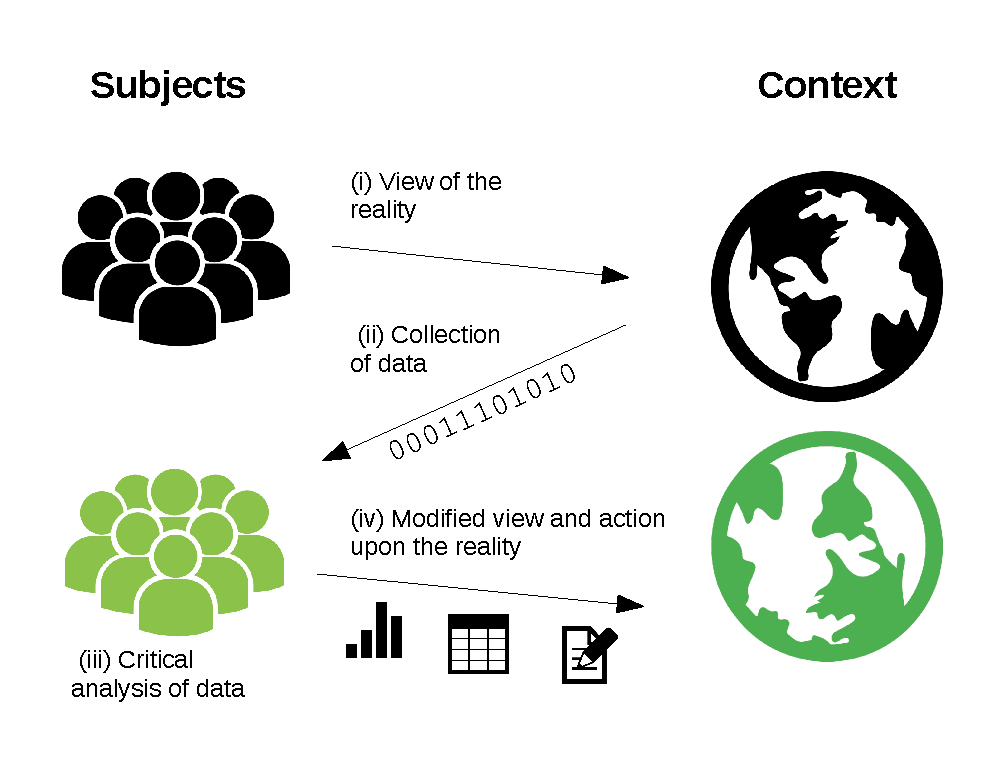
\includegraphics[width=\columnwidth]{images/critica_data_literacy}
\caption[Critical data literacy process.]{Critical data literacy process. Source:~\citeonline{Tygel2015a}}
\label{fig:critical_dl}
\end{center}
\end{figure}

\subsubsection{Data Literacy Stages}

\noindent \textbf{Investigation}

As already stated, this stage must guarantee that the educational process effectively starts from the educands reality. Just like the grape is not a typical fruit from the northeast region of Brazil, a database is also probably not something that is explicitly part of the everyday life of data educands. (Their personal data, however, are almost definitely registered in one or more databases.) At the same time, it is important to seek in the reality of each educand elements where data can be useful to understand that reality. Considering possible problems in dealing with computers, it is fundamental that the themes to be worked with are of great interest of educands, and have their foundations in daily life. It is also important to find contradictions in this reality that one desires to overcome. Thus, an interesting way of starting this quest is through statistics. For example, as detailed in~\citeonline{Tygel2015}, in a data literacy course, the educands were exposed to statistical informations previously selected about their realities. From this point on, it was shown that, on the one hand, datasets were already part of their life, and on the other hand, that much information known by the educands were omitted by data. Thereby, a data mediated world view is approached, facilitating the most adequate choice of thematic axis to work with.

\noindent \textbf{Thematisation}

At this stage, the main goal is to motivate the understanding of the world through data. Either for a local or global reality, about specific or generic themes, data allows an understanding of reality commonly seen as “neutral” or “objective”. At the thematisation stage, it is still possible to keep this aspect, which will be further deconstructed in the problematisation stage.

By elaborating thematic axes, in this stage the aim is to code certain contexts as data and aggregated information, such as statistics, graphics and tables. This coding may lead to more complex decoding about the same theme. A reality can be coded into data, which can be once more coded into aggregated information, and then can be further decoded, generating a modified view over the same reality. It is always important to notice that this process has an intrinsic bias, related to the design choices at data acquisition and processing. 

As a result of this stage, it is possible to obtain the generative themes, which in the case of data literacy, are specific context coded into data. This data can be already available as open databases, closed and subject to information access requests, or may also be uncollected data, which could provide some interesting perspectives. The final aim of this stage is to enchant educands with the world of data that represents realities.

\noindent \textbf{Problematisation}

After the “enchantment” with the world of data, it is fundamental to problematise it, i.e., to unveil what is behind the scenes when talking about data. In order to use data with critical conscience, it is necessary to know where they came from, how and to what purpose they were generated. Thus, it is possible to politicise the use of data, and deal with them not only from the point of view of a passive user, but from the perspective of someone who is also able to produce data, and with them, “say his word”. The final aim of this stage is to promote a critical view about the chosen theme, understanding the role of data for enlightening certain aspects and hide others. We list here, without any aspiration of completeness, two issues that can serve as a starting point for the problematisation stage:

\begin{itemize}
\item \emph{Non-neutrality of Data:} Data are not neutral. The seducing precision and objectivity of data grounded statements almost always hide ideologies and intentions about anything one wants to prove. Thus, it is fundamental to problematise the origin of data. Are data from the government or from civil society organizations? What was the political position of that organization at the time when data were generated? If it is about scientific data, who funded the research? More complex, but also of great importance, is the knowledge of the methodology used to gather data. Lack of awareness of the methodological approach can lead to misunderstandings and flawed conclusions. 

With that information – origin and method – it is possible to infer what was the objective of data generation, where it is not explicit. Producing data is a costly activity, which requires a considerable amount of resources, especially when dealing with big populations and/or wide areas. Therefore, every research that generates data has a very well defined purpose, which must be unveiled and discussed.

Research is designed by specific actors, to reach strategic goals. Similarly, methodologies are designed in order to highlight some aspects, and not others. This is why we can affirm that data resulting from these researches are not neutral, and therefore its non-neutrality must be problematised in a critical perspective of data literacy education.

\item \emph{Transparency:} In many cases, the critical use of data will come across the lack of available data. These missing data may not exist, be hidden or poorly organized, which is the case of many governmental data. In order to work critically with data, it is necessary to have conscience of one's rights to access information, which is directly related to transparency policies. Many countries are advancing in this field, publishing their data online and creating laws to guarantee access to information, transparency and open data, with the valuable argument of enhancing democracy and fighting corruption. However, as stated by the Global Open Data Index, only 11\% of the assessed datasets in 97 countries are open. Thus, discussing transparency and access to information is a possibility of problematising data literacy.  

\end{itemize}

\noindent \textbf{Systematisation}

The systematisation process requires data and information about an experience. In the data literacy context, the ability to put together data retrieved from various external sources with subjective qualitative information empirically obtained should be encouraged.

The systematizing stage should be the conclusion of the whole lived process – investigation, thematisation and problematisation. Of crucial importance is the communication of the results. Data can be exposed in several forms, such as graphics, tables, maps, infographics, music, film or even text. The ability to choose the right way of systematizing and communicating data is certainly a point that should be stressed in data literacy. 

\subsubsection{Definition}

Considering the arguments developed in this section, we derive our definition of critical data literacy:
Critical Data Literacy is the set of abilities which allows one to use and produce data in a critical way. This set is composed by:

\noindent \textbf{Data reading:} \emph{The ability of reading data starts at understanding how data was generated, i.e., which methodologies were used in order to capture data from a context, which facts, measures and dimensions were considered, and at which level of detail, or granularity, data was collected. It also includes understanding who produced it, in which context and why. Data should not be read as objective fact, but as the output of a social process.}

\noindent \textbf{Data processing:} \emph{The ability to technically process data is related to the use of computational and statistical tools in order to transform data into information. Linking data with other sources is also an important skill. Data should be processed based on explicit objectives.}

\noindent \textbf{Data communication:} \emph{The ability to communicate data comprises finding better matches between data types, such as distributions, temporal series, networks or comparisons, and communications tools, such as text, tables, several types of charts, maps or infographics combining these elements. Communicating data also encompasses a social evaluation of what message should be transmitted to which target audience. Data communication should be done in an ethical, responsible and precise way, in order to avoid misunderstandings or invalid conclusions.}

\noindent \textbf{Data production:} \emph{The ability to produce data includes deepening all elements within data reading. Additionally, knowledge about data formats and data publishing tools is required. Generally, data should be published not only respecting the Open Definition, but also offering tools so that non-experts are able to use it.}



\subsection{Conclusions}

The fast spreading of ICTs in the society has, as one of its consequences, a recent publication of massive quantities of data over the Web. These can be either related to governments, through public transparency initiatives, or generated by companies or civil society organizations, or even originated from scientific research. This huge mass of new information brings with it a series of potential benefits, but also major challenges, which are for the most part not as explicit as the benefits. There is an imminent risk of establishing an elite able to profit from these data, interpret it and act in the world through it, while most of the people remain excluded. In this paper, we sought in the work of Paulo Freire inspirations for the construction of a critical data literacy, which incorporates awareness of this challenge.

Future works on this topic includes deriving more tangible examples of the application of this methodology in practice, followed by developing a strategy to assess and evaluate the outcomes. From the theoretical point of view, a deep analysis of the digital literacy literature could also bring more elements for data literacy. 

It was not by accident that Paulo Freire materialized his Popular Education pedagogy into a literacy method. For him, literacy is not only useful to read words, but to read the world. And imbued precisely by this spirit, we propose an analysis of data literacy based on Freire's Literacy Method. By doing so, we hope to provide a small contribution to the democratization of access to information. Data alone do not change the world, but we believe that people who critically understand the reality through data have better tools to do it.

\section[Teaching Open Data for Social Movements: Action and Research for Open Data Engagement]{Teaching Open Data for Social Movements: Action and Research for Open Data Engagement\footnote{This section is adapted from~\citeonline{Tygel2015}}}

\label{dl_method} 

Motivated by research on use and publication of open data by social movements and grounded on popular education principles, an open data course was developed. According to the dialogicity principle, the course objective is double: (i) to tackle the issue of open data education, indicated to be one of the factors hindering the use of open data; and (ii) to use the time in training to observe the activists using data and gather information for the research.

The course programme was elaborated seeking a balance between the social aspects of the use of data, the principal motivation, and the technical issues that are inherent in the tools for data manipulation. The methodology switches between expository stages and individual and collective activities by the students. It is expected that the students can at least achieve a critical view about data, understand the possibilities and limits of its use, be aware of the political questions involved in data production and publishing, and, finally, have a technical starting point for manipulating data.

The course is divided into four stages of four hours each, but can be adjusted to needs of the people involved. A website containing teaching materials, links to data sources, and a discussion forum was developed, which in each presentation of the course is supplemented with more data.
Only two requirements are asked of people interested in attending the course: a basic knowledge of informatics (web navigation) and access to a computer (which could also be offered by the organizers). Good quality internet access provided by the organizers is also highly desirable.

\subsection{First Stage – Introduction}

The first stage starts with a short description of the course, and the participants are informed that they will also be contributing to a research project. This stage is intended to get people on the same level, by discussing the sociotechnical and political aspects of data. The aim is to start from the educands' own experience, as suggested by the Popular Education approach. For this, all participants are asked to present themselves, state their expectations and why he or she decided to take part.

Afterwards, a challenge is proposed: some socially relevant statistical results are presented (see \autoref{tab:dl_examples}), and the educands are asked to find the data sources related to those figures. Following the inverse path (information to data, rather than the opposite), we expect to raise curiosity and show, in practice, the importance of knowing what is behind the statistics.

\renewcommand{\arraystretch}{1.8}
\begin{table}[h]
\ABNTEXfontereduzida
\centering
\caption[Examples of data driven statements.]{Examples of data driven statements used to stimulate a critical view of data sources, based on Brazilian statistics agencies.}
\label{tab:dl_examples}
\begin{tabular}{ll}
\hline
\multicolumn{1}{|l|}{1} & \multicolumn{1}{l|}{0.9\% of the biggest landowners own 45\% of arable land in Brazil} \\ \hline
\multicolumn{1}{|l|}{2} & \multicolumn{1}{l|}{\begin{tabular}[c]{@{}l@{}}In Brazil, white men earn more than white women, who earn \\ more than black men, who earn more than black women\end{tabular}} \\ \hline
\multicolumn{1}{|l|}{3} & \multicolumn{1}{l|}{77\% of young people killed in 2011 in Brazil were black} \\ \hline
\multicolumn{1}{|l|}{4} & \multicolumn{1}{l|}{\begin{tabular}[c]{@{}l@{}}46.7\% of Brazilian exportation in 2013 were basic products, \\ 12.6\% were semi- manufactured, and 38.4\% were manufactured\end{tabular}} \\ \hline                                                                                    
\end{tabular}
\end{table}

In the sequel, several open data related topics are discussed:

\noindent \textbf{How does data arise:} a data path is presented, from the occurrence of something, passing through its systematization to its publication. Concepts such as facts, dimensions, and measures are discussed, together with the political motivations and consequences of those design choices. This topic is intended to put data neutrality in question, by showing that data produced by research is an outcome of several choices, made according to some goal.

\noindent \textbf{Data visualization:} the same dataset can be observed in many ways, and the conclusions to which one may come heavily depend on this. Visualizing data as tables, graphics, networks (graphs), or maps may reveal different aspects and induce several kinds of conclusions.

\noindent \textbf{Open Data:} In this topic, we motivate the understanding of open data using analogies (see \autoref{tab:open_close}). In the sequel, we define open data according to the David Eaves' three rules: data must by findable in the Web, published in machine readable formats, and cannot have licenses which prevent re-use (Eaves, 2009). A debate about linking and semantically marking data through the use of Linked Open Data (LOD) is also proposed with examples.
Transparency Policy: At this point, we present the context of open data in Brazil and in the world, especially through transparency policies. It starts with the Freedom of Information Act (FoIA), and goes up to Internet governance, with the recent Brazilian regulation1 based on three foundations: net neutrality, privacy and freedom of expression. International efforts on transparency, such as the Open Government Partnership (OGP) are also presented.

\noindent \textbf{Synthesis:} After presenting all topics, educands are asked to discuss how open data is related to their activism.

\begin{table}[]
\centering
\ABNTEXfontereduzida
\caption{Open and closed analogies to help understand what open data is.}
\label{tab:open_close}
\begin{tabular}{|l|l|}
\hline
\multicolumn{1}{|c|}{\textbf{Open}}        & \multicolumn{1}{c|}{\textbf{Closed}}           \\ \hline
Text in digital format (txt, odt, doc)     & Printed Text                                   \\ \hline
Presentation in editable format (odp, ppt) & Presentation in PDF format \\ \hline
Source code                                & Executable software                            \\ \hline
Raw Data                                   & Information (statistics, graphics, maps)       \\ \hline
\end{tabular}
\end{table}

\subsection{Second Stage – Data Sources}

The second stage of the course is dedicated to an overview of some important datasets on the Internet. It is worth noting that some of them are not “open” by the classical definition (Eaves, 2009), mainly because the raw data is not available for download. However, when an aggregate data querying system is offered, it makes data even more useful for common user than if raw data was available.

Different forms of accessing data are discussed. We recognize that, in respect to data access means, there is a trade-off between the ease of analysing data and the autonomy one can have in assessing one’s own conclusions. When a database is published as raw data, following all open data principles, this still might not help a citizen who wants to know how much was spent on education is his city. Large volumes of data coded in specialized formats (e.g. R, SPSS, SAS, SQL, XML, RDF) allow a high level of autonomy in the analysis, but special skills are needed to work with it. On the contrary, aggregate data, reports and charts allow people to have access to this information, but it has already passed through someone else's filter. Figure 1 depicts this debate. 

\begin{figure}[h!]
\begin{center}
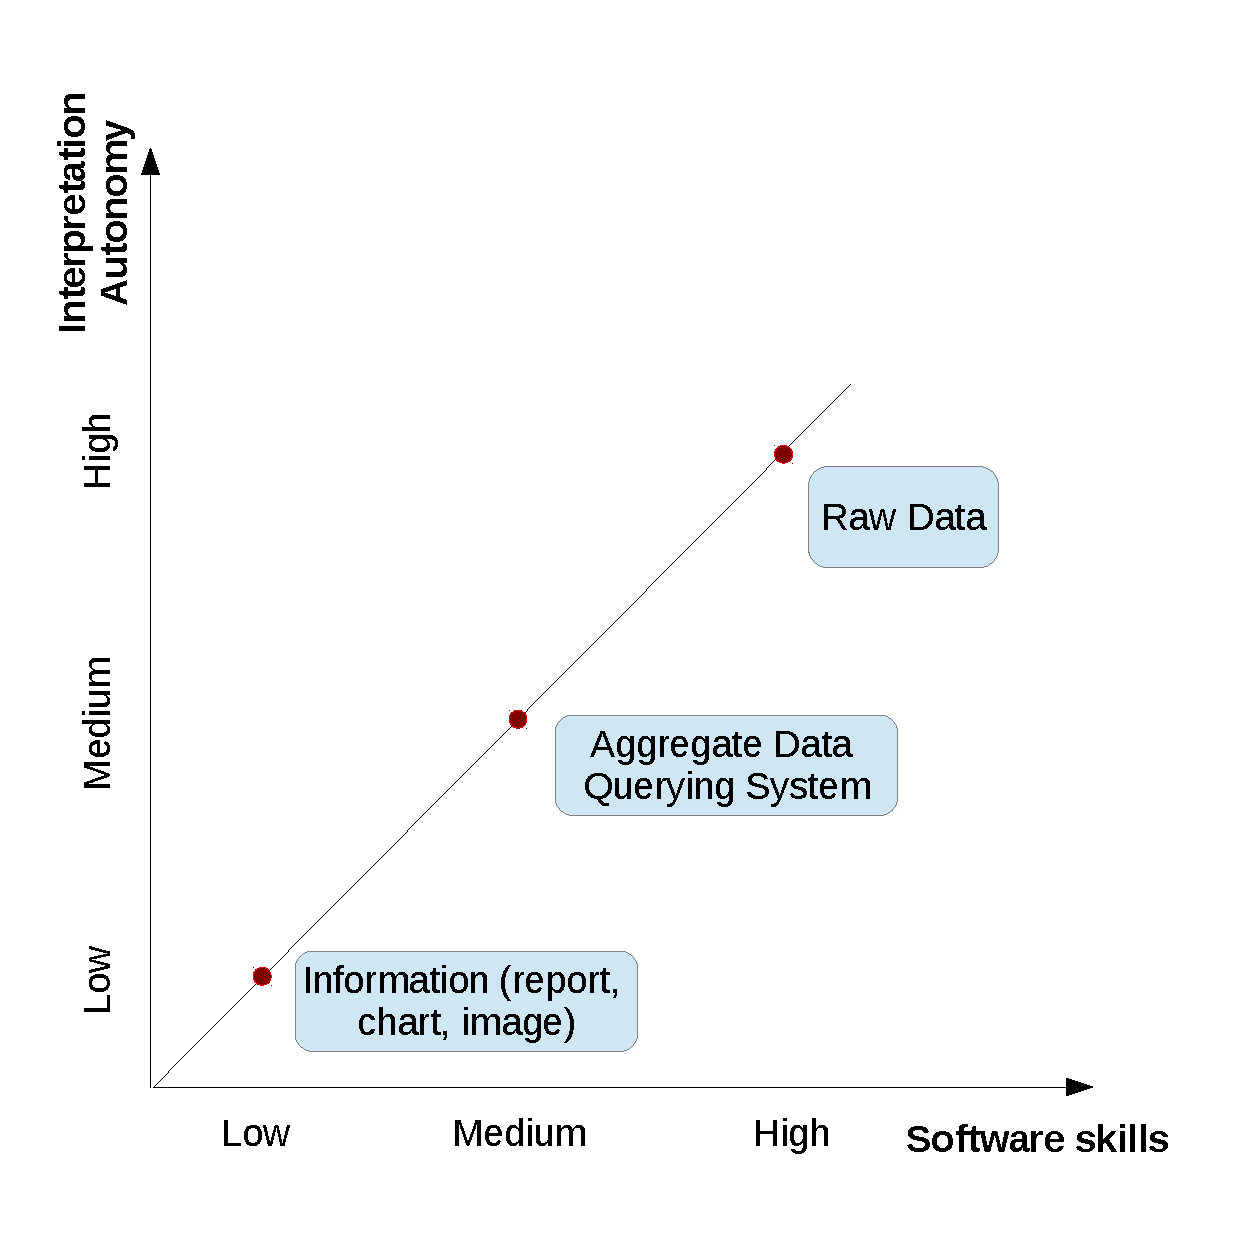
\includegraphics[width=\columnwidth]{images/opendatatradeoff.pdf}
\caption{Trade-off between interpretation autonomy and software skills needed.}
\label{fig:opendatatradeoff}
\end{center}
\end{figure}

Besides the means of data access, we propose a classification of data according to the type of provider:
Data produced by the state: This is the wider category, since the state has structural conditions and legal liability to produce data. In Brazil, the biggest data producer is the Brazilian Institute of Geography and Statistics (IBGE, in Portuguese), responsible for demographic, economic, geographic and many other sorts of data. The Unified Health System (SUS, in Portuguese) is also an important data generator, mostly about health and illnesses. Worldwide, the United Nations (UN) and the World Bank are also important data suppliers. Even though they are not governments, most of their data is compiled from country data. It is important to emphasize that this kind of data carries with it the visions and ideologies of those who generated it. All the design choices made during the data production, including definition of facts, dimensions, and measures, in some degree follows the government intentions.

Data produced by the state and shown by society: In many cases, data produced by the state is not open, and when it is open, there are no tools for the citizens to easily analyse and take their own conclusions. Specialists are needed in order to translate data into useful information. In order to tackle this issue, many society-driven applications using official data have been recently released. In many cases, they help visualize data in a way that leads to conclusions against the states' interest. One example is the Brazilian's “Congress Owners” application. Based on raw (and hard to analyse) donation data published by Electoral Justice, a civil society organization has developed an application where people can easily access and visualize the amount of donations received by politicians and parties, or paid by enterprises or economic sector. 

Data produced by society: The case where organized groups of the civil society produce their own data is interesting because: (i) as in the case of state data, data produced by the civil society contains its ideological influences in the design choices; (ii) it allows other perspectives on subjects already explained by the state. 

Data related stories can oppose well established hegemonic opinions. One example is the Brazilian Map of Environmental Injustice. Agribusiness is considered to be a good development alternative for the country, based on its relevant contribution to the gross domestic product. The map shows 82 occurrences of Environmental Injustice related to the agribusiness (from a total of 501), where activities of this sector cause damage to poor communities and/or to the natural habitat. \autoref{tab:sm_initiatives} shows a number of society driven databases. It is worth noting that, in some cases, the funding for building those databases comes from the Government. In principle, we consider that this does not hurt society’s autonomy and freedom to put their views forward in the design process.


\begin{table}[]
\centering
\ABNTEXfontereduzida
\caption[Examples of society driven databases.]{Examples of society driven databases, used by social movements with several purposes.}
\label{tab:sm_initiatives}
\begin{tabular}{|l|l|}
\hline
\multicolumn{1}{|c|}{\textbf{Initiative}}  & \multicolumn{1}{c|}{\textbf{Publisher}}  \\ \hline
\begin{tabular}[c]{@{}l@{}}\href{http://www.conflitoambiental.icict.fiocruz.br/}{Environmental} \\ Injustice Maps\\  (Brazil)\end{tabular} & Fiocruz and FASE                                                                                                                            \\ \hline
\begin{tabular}[c]{@{}l@{}} \href{http://conflitosambientaismg.lcc.ufmg.br/}{Environmental} \\ Conflicts Maps \\ (Minas Gerais, \\ BR)\end{tabular}       & \begin{tabular}[c]{@{}l@{}}Federal University of Minas Gerais, \\ Brazil (in partnership with a number \\ of social movements)\end{tabular} \\ \hline
\begin{tabular}[c]{@{}l@{}} \href{http://www.ejolt.org/maps/}{Atlas of} \\ Environmental \\ Justice\end{tabular} & \begin{tabular}[c]{@{}l@{}}23 worldwide organizations (see \\ http://www.ejolt.org/section/team \\ for a complete list)\end{tabular}        \\ \hline

\href{http://agroecologiaemrede.org.br}{Agroecology initiatives}  & \begin{tabular}[c]{@{}l@{}}ANA/ABA (Brazilian national social \\ movements related to agroecology)\end{tabular}                             \\ \hline
\href{http://cptnacional.org.br/}{Land Conflicts} & Comissão Pastoral da Terra (CPT)                                                                                                            \\ \hline
\end{tabular}
\end{table}

In the final activity of this stage, educands are asked to add new data sources to the course web page, according to their interests. New sources can come from students' experiences, or be searched for during the class time. However, it is important to find the exact link, since this is reported to be a difficulty, as it will be seen later.

\subsection{Third Stage – Tools}

In the third stage, the focus is on tools for manipulating data. The goal is to present the means to work with the raw or aggregate data resulting from queries. It begins with an introduction to the Comma Separated Values (CSV) format, which is an open, universal and easy-to-use way of exchanging tabular data. Concepts such as primary and foreign keys are also discussed, in order to help comprehend how relationship between tables and databases can be made. Nevertheless, database design is beyond our scope.

This is an essentially practical stage. Several tools are presented, so that each student can choose which one he or she wants to work with, according to individual interests and ability with computers.

The first tool presented is a spreadsheet editor. The task consists in downloading a CSV sheet with a two dimensional table (production of food in tons, by type of food and year) and drawing a line chart. Students are also asked to plot percentage changes between first and last year production. The second part of the task consists in working with dynamic tables, which allows building analysis frameworks with more than two dimensions.

Other tools presented are related to map building and infographics drawing. Sometimes a mathematical background revision is necessary, since working with number variations requires some previous knowledge of percentages.

\subsection{Fourth Stage – Final Work}

The fourth and final stage is dedicated to a jointly decided activity. The goal is to develop some data based communication product, based on the three previous stages. Ideally, there should be more than one facilitator in the room, so that the work can be divided into groups, with each group being accompanied by one instructor.

Suggested options include: writing news text based on data, and building infographics and maps on specific subjects. The intentionality – what and why we want to communicate – is discussed first. Then, we evaluate the feasibility of the task – is there data about this subject? – and finally, the communication instrument is chosen. In the end, results are presented and an evaluation of the course is done.

The next section brings an analysis of presentations of this course, and draws out some research results based on the experiences gained.

\section[Open Data Clues from the Field]{Open Data Clues from the Field\footnote{This section is adapted from~\citeonline{Tygel2015}}}

\label{dl_results} 

In this section, we describe the application and the systematized results of the above detailed open data course.

The course was presented five times in the second semester of 2014, in Brazil. While three presentations happened in Rio de Janeiro, one was held in Vitória (state of Espírito Santo) and another in Porto Alegre (state of Rio Grande do Sul). Two presentations were held in a workers union and three in universities, organized by groups who work with social movements in extension projects. A total of 52 students enrolled and participated in at least one stage. There were no fees to pay, and the only requirements were basic informatics knowledge and access to a computer, sometimes provided by the organizers. \autoref{tab:dl_summary} shows a summary of the presentations.

\begin{table}[]
\centering
\ABNTEXfontereduzida
\caption{Summary of the presentations of the open data course for social movements.}
\label{tab:dl_summary}
\begin{tabular}{|l|l|l|l|l|l|}
\hline
\textbf{N.} & \textbf{\begin{tabular}[c]{@{}l@{}}Kind of \\ Place\end{tabular}} & \textbf{City}                                             & \textbf{\begin{tabular}[c]{@{}l@{}}Duration (h) and time\\ distribution\end{tabular}} & \textbf{\begin{tabular}[c]{@{}l@{}}Participants\\ enrolled\end{tabular}} & \textbf{\begin{tabular}[c]{@{}l@{}}Forms\\ responded\end{tabular}} \\ \hline
1           & Union                                                             & \begin{tabular}[c]{@{}l@{}}Rio de \\ Janeiro\end{tabular} & 16h (four days at night)                                                              & 6                                                                        & 2                                                                  \\ \hline
2           & University                                                        & \begin{tabular}[c]{@{}l@{}}Rio de \\ Janeiro\end{tabular} & 16h (two full days)                                                                   & 11                                                                       & 3                                                                  \\ \hline
3           & University                                                        & Vitória                                                   & 16h (four days at night)                                                              & 13                                                                       & 4                                                                  \\ \hline
4           & University                                                        & \begin{tabular}[c]{@{}l@{}}Porto \\ Alegre\end{tabular}   & \begin{tabular}[c]{@{}l@{}}12h (one half day/one \\ full day)\end{tabular}            & 12                                                                       & 3                                                                  \\ \hline
5           & Union                                                             & \begin{tabular}[c]{@{}l@{}}Rio de \\ Janeiro\end{tabular} & 8h (two days at night)                                                                & 10                                                                       & 3                                                                  \\ \hline
\multicolumn{3}{|l|}{\textbf{Total}}                                                                                                        & \textbf{68 h}                                                                         & \textbf{52}                                                              & \textbf{15}                                                        \\ \hline
\end{tabular}
\end{table}
The analysis will be based on two instruments: an evaluation questionnaire that all students were asked to fill in, and a participant observation gathered during the presentations. The goal of the analysis is to respond to the research questions: (i) why social movements use data (motivations); (ii) what are the mains problems (impediments); and (iii) what could be done to enhance the use (improvements). Also, the evaluations about the course can be used to improve it.

\subsection{Questionnaire Based Analysis}

All the participants were requested to answer a questionnaire after attending the course. Thus, we assume that the opinions given are strongly influenced by the discussions held over the course. This decision was taken having in mind that: (i) open data is not a subject of the educands' everyday life; so, answering before the course could lead to meaningless results; (ii) according to the popular education methods, we expect each educand to be able to relate content unseen before with their experiences, and in the end to synthesize their own conclusions about the process. 
\autoref{tab:questions} shows the questionnaire and the mean, maximum, and minimum values for numerical questions.

\begin{table}[]
\centering
\ABNTEXfontereduzida
\caption[Questionnaire answered by course attendants.]{Questionnaire answered by course attendants. All the numerical results are in over a base of 15 (n = 15), and N/A means “not applicable”.}
\label{tab:questions}
\begin{tabular}{|l|l|c|}
\hline
\multicolumn{1}{|c|}{\textbf{\#}} & \multicolumn{1}{c|}{\textbf{Question}}                                                                                                   & \textbf{\begin{tabular}[c]{@{}c@{}}Mean \\ (maximum \\ - minimum)\end{tabular}} \\ \hline
1                                 & Age                                                                                                                                      & 31 (25–48)                                                                      \\ \hline
2                                 & Knowledge of informatics (1: poor knowledge – 5: good knowledge)                                                                         & 2.7 (1–5)                                                                       \\ \hline
3                                 & Work/Profession/Activism                                                                                                                 & N/A                                                                             \\ \hline
4                                 & \begin{tabular}[c]{@{}l@{}}Why have you attended to the course? Why do you think open data \\ is important?\end{tabular}                 & N/A                                                                             \\ \hline
5                                 & \begin{tabular}[c]{@{}l@{}}Educator's performance (didactics, material, knowledge, punctuality) \\ (1: poor – 5: very good)\end{tabular} & 4.5 (3–5)                                                                       \\ \hline
6                                 & \begin{tabular}[c]{@{}l@{}}Self performance (participation, attention, punctuality) (1: poor – 5: \\ very good)\end{tabular}             & 3.3 (1–4)                                                                       \\ \hline
7                                 & \begin{tabular}[c]{@{}l@{}}Was the subject according to your expectations? (1: totally distinct – \\ 5: totally according)\end{tabular}  & 4.6 (2–5)                                                                       \\ \hline
8                                 & What is the main impediment perceived by using data?                                                                                     & N/A                                                                             \\ \hline
9                                 & How do you imagine that the use of data could be improved?                                                                               & N/A                                                                             \\ \hline
\end{tabular}
\end{table}
The median age of participants was 31 years, with the youngest being 25 years old and  the oldest 48. They considered themselves to have medium knowledge of informatics. Before enrolling, participants were asked to have some informatics knowledge, but no admission tests were given.

Some participants were exclusively activists or academics, but most of them were activists with some academic involvement. There were journalists, lawyers and social scientists, all engaged with some social movement. No participant had formal informatics training, meaning that no one was an informatics expert.

The teacher's performance was well rated, but this was somehow expected in a free course. On the other hand, no one rated him or herself with very good participation performance. In Question 7, only one participant seemed to have very different expectations about the course content. All the others marked 4 or 5, indicating that open data is not so distant from non-informatics people's lives, at least for those who answered the questionnaire.

In order to analyse questions 4, 8 and 9, we will pick answer elements and classify them according to research 
goals: motivations, impediments, and improvements. Question 4 was aimed to catch motivations, but impediments and improvements were also cited. Question 8 raised only impediments, and Question 9 only improvements, as intended.
An effort was made to extract concrete elements from the discursive text. An equilibrium was sought between merging similar statements and not losing the diversity of opinion. These concrete elements extracted can be seen in \autoref{chap:dl_results}., in Tables~\ref{tab:dl_results1}, \ref{tab:dl_results2}, and \ref{tab:dl_results3}.

Sometimes, the separation between the classes is not very clear. All impediments (e.g. “Open Data Portal is hard to use”) have implicit improvements (e.g. “Open Data Portal could improve usability”), as all improvements also have implicit impediments. Some motivations (e.g. “Use spending data to fight corruption”) also could be interpreted as impediments (e.g. “Few spending data is available”) or improvements (e.g. “More spending data must be made available”). We tried to classify according to the respondent's intention.

\subsection{Observation Based Analysis}
\label{sec:obs_based_analysis}
In this section, some remarks are made based on the 68 hours observation of the course. This observation was driven inspired by the ethnographic method of participant observation~\cite{Atkinson1994}. Within this approach, the researcher plays an established participant role in the studied scene, in this case, as an educator, taking field notes during the class. Ethnography inspired methods are complementary to objective and quantitative evaluations since, according to~\citeonline{Atkinson1994}, ethnography deals with the “analysis of data that involves explicit interpretation of the meanings and functions of human actions”, and “represents a uniquely humanistic, interpretive approach, as opposed to supposedly 'scientific' and 'positivist' positions.” Since two of our research questions deal with human actions and feelings – what are the motivations of social movements for using open data and what are impediments that block a wider and better use – we considered the participant observation an appropriate methodological direction. We aimed to comprehend the point of view of the educands, and this was done from the educator stance, which certainly influenced the analysis.

As described earlier, in the first stages of the course participants are shown statistical statements (see \autoref{tab:dl_examples}) and are asked to search for data that generated those figures. Below, we list some behaviours observed:

\begin{itemize}
\item The first impulse of users is to paste the phrases directly into a web search engine. Normally, the results are news commenting that statement, or reports containing that information, and never the actual data source.
\item For some people, it is difficult to understand the difference between the statements and the data sources from which they were originated. One way to overcome this misunderstanding is to slightly rephrase the statement and ask what would be the new figures. For example, relating to statement 1 (Listing 1), we would ask: “how much land do the 0.1\% of the biggest landowners possess?”.
\item Overall, only few people reached the actual data source. This shows that one of the main problems of data sets and their query/download systems is that they are frequently hidden in the deep web, i.e., regular search machines cannot find them.
\end{itemize}

In the second stage of the course, some data sources are presented and divided into three categories. About this stage, we would like to remark:

\begin{itemize}
\item In general, although interested, users are unfamiliar or unaware of data sources. This ignorance is, as expected, worse for society driven OGD based applications, and for data produced by social movements, which usually have no official means of dissemination;
\item Students were stimulated to add new data sources to the course website, according to their own interests or activism. In some cases, participants inserted already known data sources, but in most cases data sources were found during the activity.
\end{itemize}

The third practical stage revealed one of the strongest difficulties in open data usage: the manipulation of software tools, particularly of spreadsheets. The knowledge about CSV tabular files, considered as a fundamental skill to use data on different systems, was practically absent. This problem got even worse because of the inability of the most-used proprietary spreadsheet application (MS Excel) to deal with such kind of file. LibreOffice, its open source counterpart, facilitates this task.

Another issue that was highlighted at this stage was the mathematical difficulty faced by most of the students. Dealing with statistical open data requires, most of the time, simple mathematical operations. Therefore, sometimes a small revision of percentage was necessary.

Unfortunately, the fourth stage of the course did not work as expected. This stage was only reached in two of the five presentations described in \autoref{tab:dl_summary}. In the first one, students, mainly journalists, decided to individually write stories and impressions about open data. They were published in the course website. The second experience reached closer to the goal: participants decided to investigate a local case of environmental injustice. Data about enterprises, population health, environmental licensing and other issues were gathered, but no final product was obtained. In the remaining three presentations, the time ran over twice, and once the students said they were tired, as this course was run on two full days, at a weekend.

One possible way to overcome this issue is to propose this work at the beginning of the course and organize tasks during the other stages. This has the advantage of motivating students with a concrete problem during the course. Nevertheless, the challenge remains: how to prepare the course without predefining the problem. Another option would be to increase the number of hours, which would depend on participants' availability.

\subsection{Synthesis}

As explained above, by a simple rephrasing, an impediment or a motivation can turn into an improvement. By doing a careful analysis of Tables~\ref{tab:dl_results1}, \ref{tab:dl_results2}, and \ref{tab:dl_results3} (see the Appendix), an improvement classification tree was built. It is aimed at orienting actions for the engagement of social movements in open data in the Brazilian context. The classification tree can be seen in \autoref{fig:dl_results}.

\begin{figure}[h!]
\begin{center}
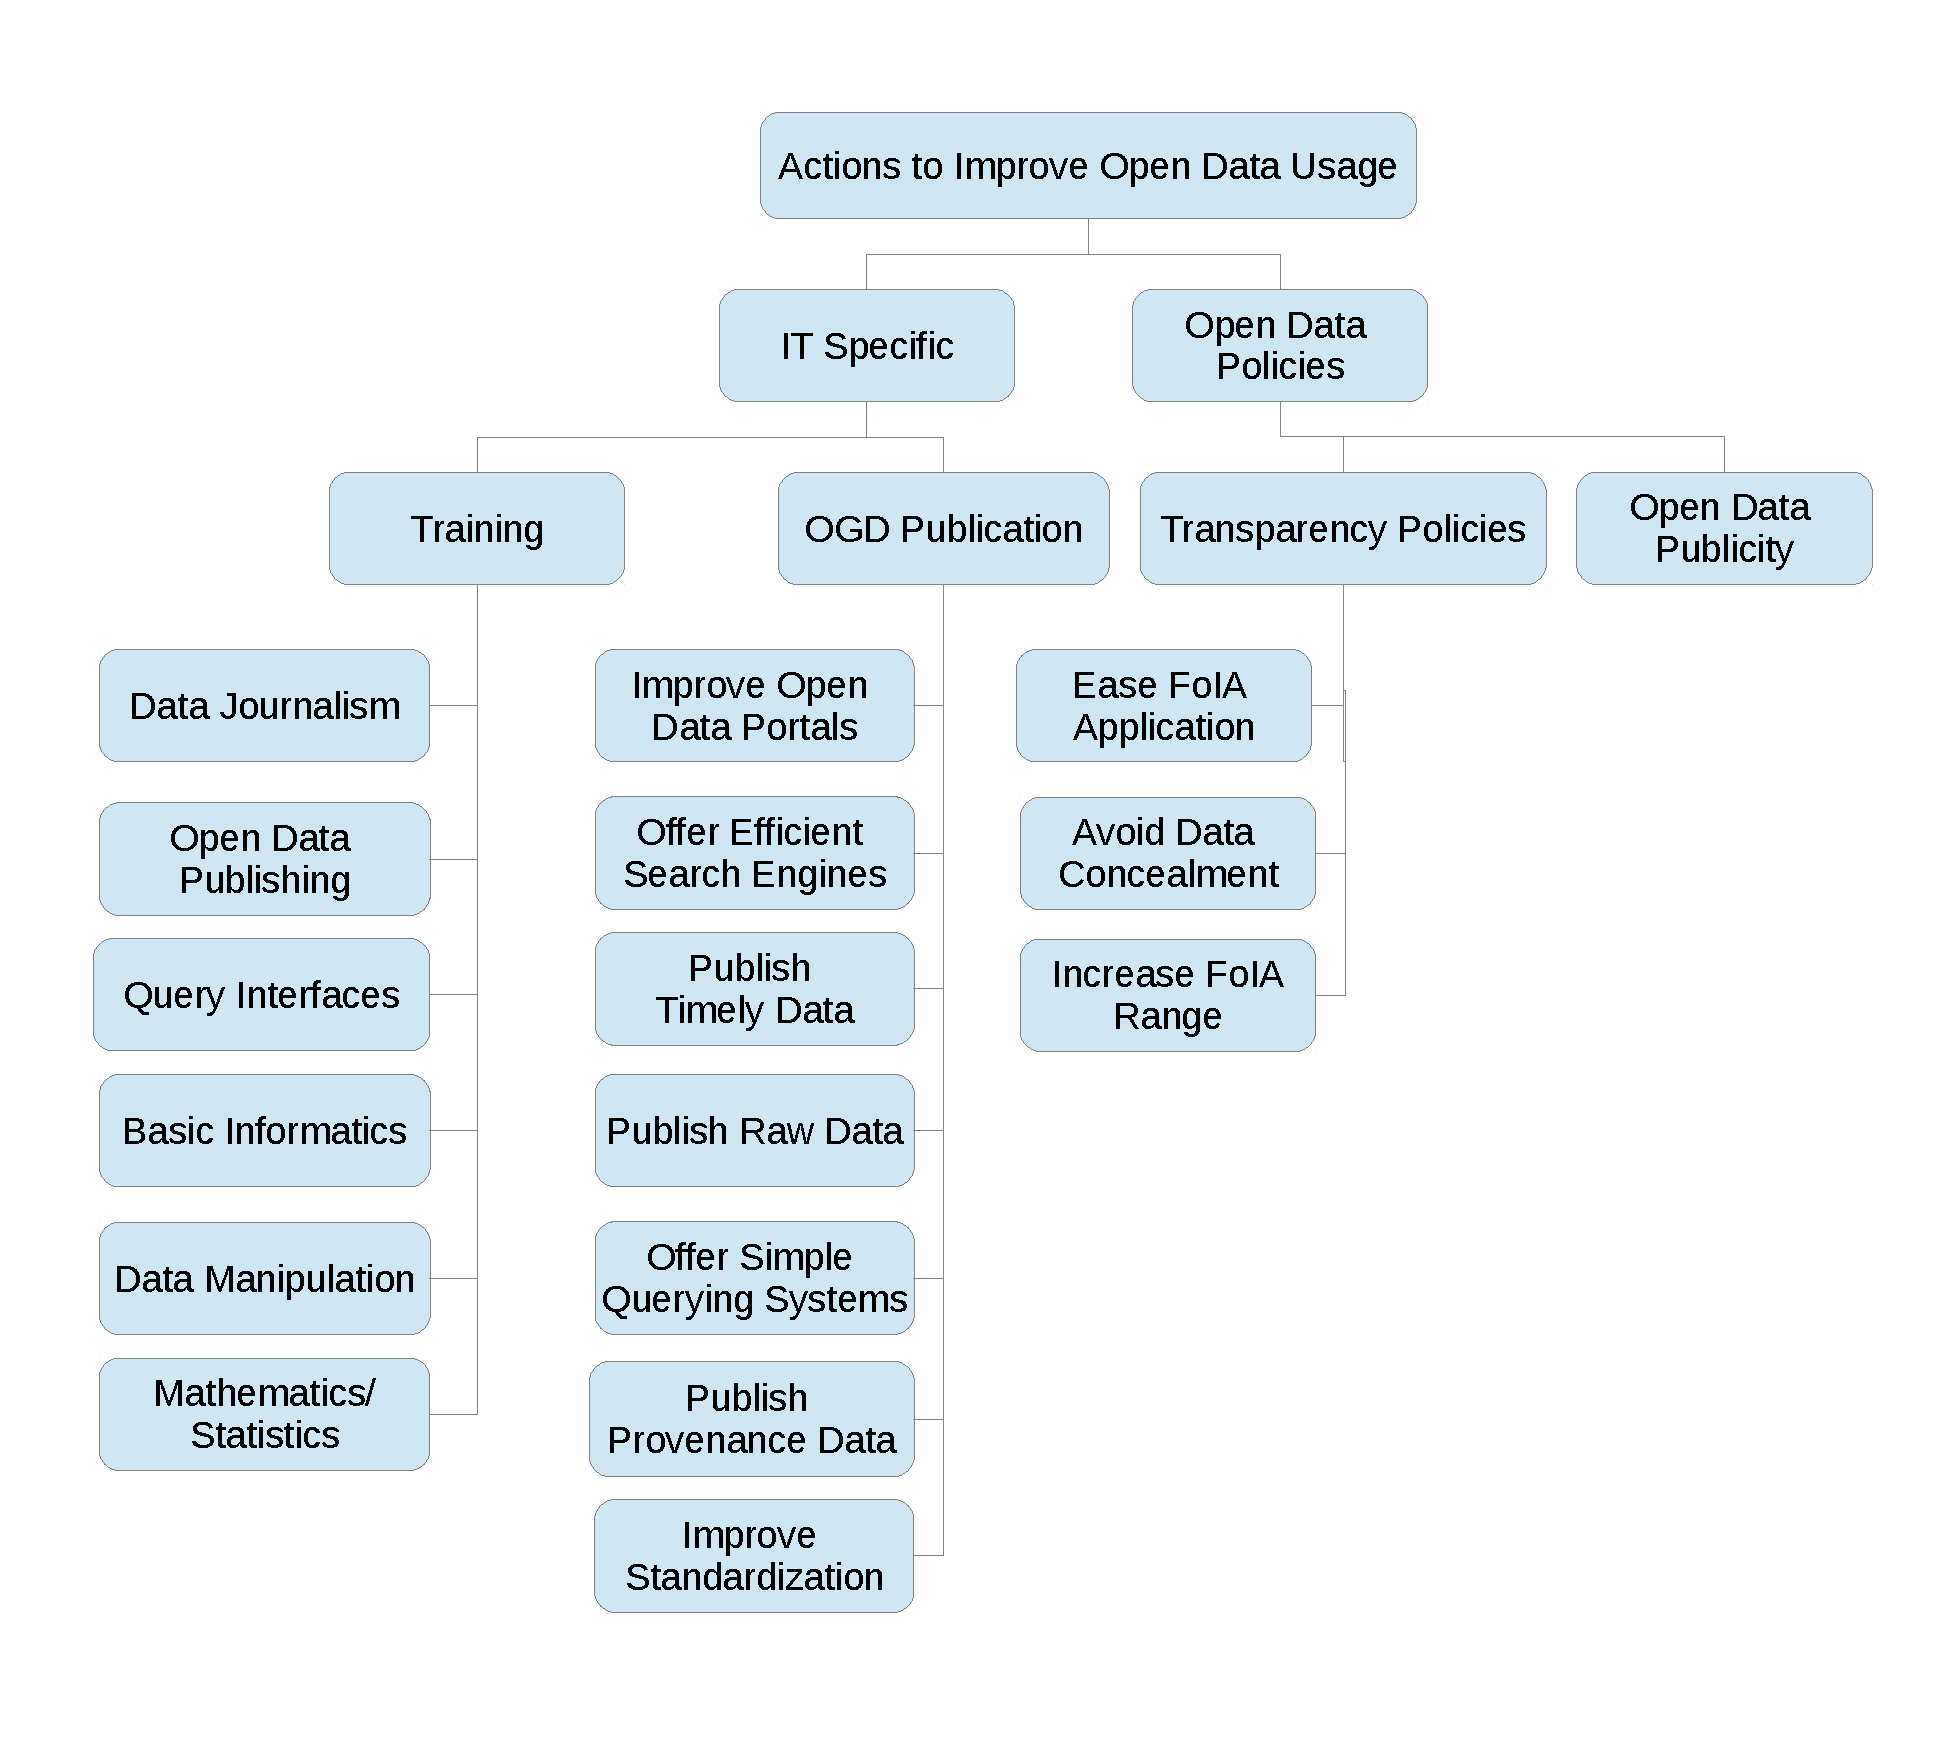
\includegraphics[width=\columnwidth]{images/impediments_classification.pdf}
\caption[Classification tree for open data engagement actions.]{Classification tree for open data engagement actions, systematized from Tables 6, 7 and 8.
The first classification is a distinction between Information Technologies (IT) Specific and Open Data Policies related issues. There is no intention to imply a duality between social and technical issues, however, one can easily recognize that some elements are directly related to information technology, and others are not.
}
\label{fig:dl_results}
\end{center}
\end{figure}


The IT Specific issues are divided into Training and Open Government Data (OGD) Publication. The first class encompasses cited impediments which could be approached with educational investments, and the second is related to actions to be taken by government data publishers. Our proposed course tackles all cited educational demands, except data publishing, since it still demands a higher level of informatics knowledge.  As to OGD Publication related issues, the need for better search engines was the most cited enhancement.

The right side of the tree presents general issues related to Transparency Policies and Open Data Publicity. We can conclude that in order to improve open data usage, actions must be taken far above data level. In this case, the whole structure for information access must be enhanced. Difficulties in claiming the FoIA within local government levels were reported, as well as accessing information on private foundations that run on public money. Finally, many participants suggested that more publicity on open data already available would also improve usage.

%\subsection{Comments}

%This section described a methodological strategy used in research on Open Data and Social Movements. An open data course was proposed in order to help understand the motivations for the use of open data by social movements, the impediments to succeed with this, and the improvements that could help the engagement of society by means of open data.

%The results of five presentations of the course were organized into a classification tree of possible open data engagement actions, shown in Figure 2. Training related actions should be fostered as part of a Transparency Policy, but social movements should also prioritize open data in their agenda.

Some improvements related to OGD publication could be addressed by using new technologies being developed under the Linked Open Data (LOD) framework. By semantically annotating data with commonly used vocabularies and ontologies, the LOD approach offers the technical means to link different data sources and jointly query them. A solid set of tools to implement LOD is being developed~\cite{Auer2014}, but strong efforts must be made to hide the complexity of the representation and to highlight its benefits, so that it can be recognised as a viable option. Other improvements are only possible through the effective political willingness of governments to be transparent.

As a methodological approach for research in informatics, the course was found to be an efficient tool, since it accomplished its dialogical function indicated by the Popular Education theory. At the same time as they were subjects on an open data education action, the educands that participated on the course acted as objects in a research project. On one side the dialogical approach resulted in a set of appointments for open data publishers; on the other side, in a satisfactory educational experience, as shown by the good educator evaluation (\autoref{tab:questions}) and by the rich answers collected (Tables~\ref{tab:dl_results1}, \ref{tab:dl_results2}, and \ref{tab:dl_results3}).

%The open data engagement actions gathered here are not supposed to be complete. The methodology used to raise these actions allows only to affirm that they can improve the use of a specific actor, a social movement, that thinks about open data with a special intentionality. Nevertheless, our efforts add to a number of other initiatives~\cite{Atz2015, Davies2013,Gurstein2011, Ubaldi2013, Veljkovic2014, Zuiderwijk2014}, encompassing other actors, and aiming to picture a desired open data scenario in the future.

\section{Conclusions}
\label{dl_conclusion} 

In this chapter, we presented both a participatory research on open data and theoretical and practical contributions to data literacy.
Together with the open data landscape presented in the previous chapter, we formed a solid view over the question dealt in this thesis. 
Considering that open data organization is an important question that hinders the achievement of open data promises, in the next chapters we will present a related approach.
The following chapter presents a literature review on methods for dealing with semantic metadata, and an analysis of the use of metadata in ODPs. 
The intention is to prepare the ground for presenting the Semantic Tags for Open Data -- STODaP -- approach, in \autoref{chap:tagging}.


\chapter{Semantic Metadata for Open Data Description}
\label{chap:relworks}

In the previous chapter, the issue of building open data skills was tackled through the development of a data literacy course as part of a participatory research.
One of the results of this research pointed out a significant problem related to the organization of ODPs.
Following this motivation, we investigate in this chapter the issue of metadata for open data. 
The chapter is divided in two parts, covering:

\begin{itemize}
	\item A literature investigation over the possible strategies to deal with semantic metadata for organization of open data repositories;
	\item An analysis of the current usage status of metadata in ODPs.
\end{itemize}

Particularly, in the first part we selected works related to semantic enrichment of metadata in ODPs, in order to position the main contribution of this thesis presented in the following chapter.
Section starts with some preliminary discussions regarding semantics and metadata.
Then, a characterization of our contribution is driven, in order to delimit the related research topics.
After this characterization, we present in each section one topic, highlighting the main related works, their gaps and relations to this work.
We start with Assessment of Metadata in \autoref{sec:metadata_assessment}, followed by Metadata Cleanup in \autoref{sec:metadata_cleanup}, Metadata Reconciliation in \autoref{sec:metadata_reconciliation} and finally with Structure Emergence in \autoref{sec:emergence}.

The second section aims to bring light over the current status of metadata usage in Open Data Portals.
Based on the CKAN Census of ODPs, we profile 87 portals and analyse several aspects regarding metadata.
The analysis embraces not only local aspects regarding individual portals, such as use, reuse and similarity within a portal (\autoref{sec:local_metrics}), but also global features between portals, such as coincident metadata and expressiveness (\autoref{sec:global_metrics}).

We conclude in the last section with an evaluation of the literature gaps and the actual problems detected in ODPs, pointing out our strategies to be developed in the next chapter.

\section{Semantic Metadata: A Literature Review}
\label{sec:semantic_metadata}

\subsection{Introduction}

It is unnecessary to argue that good metadata are crucial for making data usable.
By \emph{good} we can give as example a series of quality attributes such as clean, well organized, detailed, complete, accessible, and meaningful.
Intuitively, metadata are meaningful if they bring new information -- meaning -- for data.
If a consumer asks: ``Which bananas do you have?'', and the seller answers: ``The yellow one!'', this is barely meaningful, since almost all types of banana are yellow.
However, if the seller answers: ``I have \emph{Cavendish}, \emph{Gros Michel}, \emph{Latacan}, and \emph{Cambuta}, which one do you prefer?'', there is much more information accessible through the types of bananas, including colour, size, countries of origin, among others.

In the Web context, the way of enhancing the meaning of an object is to connect it to the Semantic Web, through the Linked Open Data Cloud, as detailed in \autoref{sec:LOD}.
This procedure is also called Semantic Enrichment or Semantic Lifting.
A special type of metadata is lately of particular interest for semantic lifting: tags, free-text labels that can describe several aspects of data.
There are two particularities regarding tags that make them interesting for semantic processing: (i) the ease of input, because there are usually no constraints for users typing tags; and (ii) the social architecture, that allows different users to tag the same data element.
Combination of both aspects results in large social tagging sets, which are also called folksonomies.
	\citeonline{Limpens2013} state a series of motivations for semantically enriching tags in the context of folksonomies, considering data generators, data curators and end-users:
\begin{enumerate}
	\item enriching tag-based search results with spelling variants and hyponyms\footnote{In linguistics, hyponyms are words that share the same type-of relationship with an hypernym. Using the bananas example, Cavendish and Latacan are hyponyms because both are types of bananas, their hypernym.};
	\item suggesting related tags to extend the search;
	\item semantically organizing tags to guide novice users in a given domain more efficiently than with flat lists of tags or occurrence-based tag clouds; and
	\item assisting disambiguation.
\end{enumerate}

A more detailed view about problems caused by the absence of semantics in metadata is described by~\citeonline{Marchetti2007}.
According to the authors, there are six categories of problems:

\begin{citacao}
\begin{enumerate}
\item \textbf{Polysemy:} the same word can refer to different concepts (the word ’field’ can refer to a piece of land cleared of trees and usually enclosed, but also to a branch of knowledge);
\item \textbf{Synonymy:} the same concept can be pointed out using different words (’auto’, ’car’, ’machine’ are three different words that refer to the same concept: a four wheels vehicle);
\item \textbf{Different lexical forms:} the same concept can be referred to by different noun forms, for instance plural nouns (’car’/’cars’), different verb conjugation (’buy’/ ’buying’), name-adjective couple (’energy’/’energetic’), multiple words (’pc’/’personal computer’) and so on;
\item \textbf{Misspelling errors or alternate spellings:} typing errors that occurs when we write a word (’staton’ in place of ’station’) or different possible spelling of the same word (’color’/’colour’);
\item \textbf{Different levels of precision:} the specificity of the word chosen to tag a resource (’jazz’ is more specific than ’music’);
\item \textbf{Different kinds of tag-to-resource association:} implicit kinds of relations that links a tag to a specific resource (’interesting’ expresses an opinion on the resource, ’car’ expresses the topic of the resource and so on) \cite[p.2]{Marchetti2007}.
\end{enumerate}
\end{citacao}

Around ten years ago, discussions about semantifying folksonomies started.
Probably one of the most important work at that time was \emph{Ontology of Folksonomy: a mash-up of Apples and Oranges}~\cite{Grubber2007}.
This work, published first on the web in November of 2005, aimed to clear up a false contradiction between ontologies, as the enabling technology for sharing sharing information on the Semantic Web, and folksonomies, a typical phenomenon of the Social Web representing data emerged from shared information.
It is perfectly reasonable that these two concepts could be understood as contradictory: while ontologies are formally built by domain experts and ontology engineers, folksonomies are freely constructed by users.
After clarifying the role of each concept, Grubber defines the ontology of folksonomy, whose central element is \emph{Tagging}, which is an activity involving an object $O$, an user $U$, a tag $T$ and a system $S$.
The possibility of qualifying a tagging is also mentioned, for example, by allowing the community to give a negative polarity for a tagging made by a spammer.

Another important work introducing this topic is \emph{``Ontologies are us: A unified model of social networks and semantics''} \cite{Mika2007}, also published first in November of 2005.
Mika also disagrees that ontologies and folksonomies are contradictory, but differently from Grubber, for who both are distinct concepts (Apples and Orange) that can be united, he states that ``folksonomies are ontologies''.
In order to justify it, author cites a set of broad ontology definitions, and classifies folksonomies in these definitions as ``lightweight, dynamic and limited in sharing scope''.

In the sequence of these papers, several authors tried to define tagging ontologies.
\citeonline{Wu2006} added a time dimension to the tagging model.
And to the best of our knowledge, \citeonline{Newman2005} was the first to propose an ontology for tagging.
This work was further extended by \citeonline{Knerr2006}, who proposed the Tagging Ontology, depicted in \autoref{fig:tagging_ontology}.
All dimensions proposed by \citeonline{Wu2006} and \citeonline{Grubber2007} are present and further detailed in this ontology.
The central element is the tagging, which acts as an event joining a tag, a tagger, a domain and a resource, as well as other optional attributes.

\begin{figure}[t]
\begin{center}
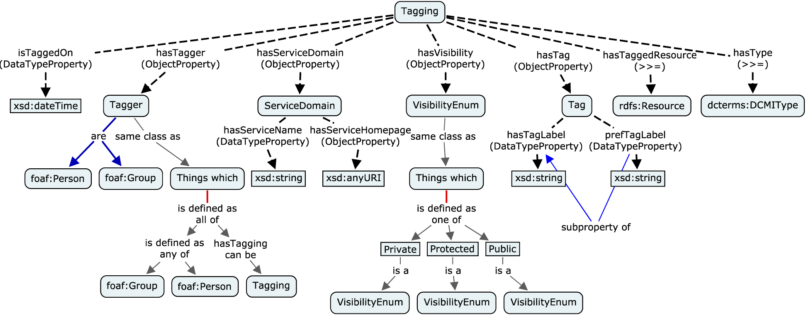
\includegraphics[width=\columnwidth]{images/tagging_ontology.png}
\caption[Tagging Ontology.]{Tagging Ontology. Source: \citeonline{Knerr2006} }
\label{fig:tagging_ontology}
\end{center}
\end{figure}

Although crucial, these models are not aimed at solving the problem of creating domain ontologies emerged from collaborative tagging.
\citeonline{Halpin2007} analysed the dynamics of collaborative tagging, in order to determine the possibilities of extracting knowledge.

It is important to notice that until this point, tagging ontologies were concerned with organizing the knowledge contained in the tagging activity.
The MOAT architecture was the first to explicitly include the concept of tag meaning, associating each tagging element to a LOD resource~\cite{Passant2008}.

A review about semantic tagging initiatives by \citeonline{Kim2008} compared the different types and relations proposed by the works until 2008, and was updated by \citeonline{Kim2011}.
In the first work, seven models were compared, using as criteria their suitability to represent tagging activities, or to represent features of folksonomies.
Authors conclude that SCOT\footnote{Available at \url{http://rdfs.org/scot/spec/}.} ontology is the only one that presents a higher level of sophistication in both directions.
The most recent attempt to build a tag ontology is the Modular Unified Tagging Ontology (MUTO)\footnote{Available at \url{http://muto.socialtagging.org/core/v1.html}}, shown in \autoref{fig:muto}, and described by~\citeonline{Lohmann2011}.
It incorporates suggestions of several previous models into a unified model, and is strongly based on wide used ontologies, such as Dublin Core, SKOS and SIOC.
An important highlight of MUTO is the possibility of connecting a meaning (an RDF resource) to a tag through the \texttt{muto:tagMeaning} property, as introduced by the MOAT ontology.

\begin{figure}[t]
\begin{center}
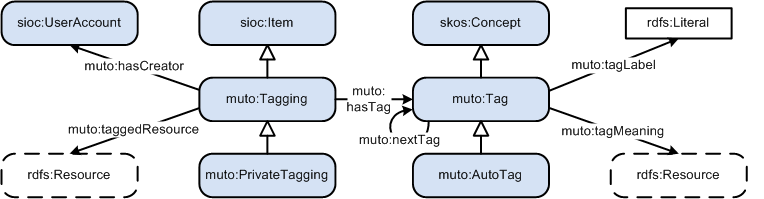
\includegraphics[width=\columnwidth]{images/muto.png}
\caption[MUTO Ontology.]{MUTO Ontology. Source: \citeonline{Lohmann2011}}
\label{fig:muto}
\end{center}
\end{figure}

Finally, in the context of tagging semantics, it is also important to discuss the nature of the relation between tags and tagged resources.
To the best of our knowledge, none of the proposed tagging ontologies incorporates the possibility of qualifying this relationship.
\citeonline{Marchetti2007} point out the question of ``implicit kinds of relations that links a tag to a specific resource'' with an example: ``\emph{interesting} expresses an opinion on the resource, \emph{car} expresses the topic of the resource.''

\subsection{Characterization of the Contribution}

The main contribution of this thesis is a semantic approach for organizing metadata in Open Data Portals, specifically regarding tags.
Thus, the following topics are considered to be related works, and will be analysed in the following:
\begin{itemize}
	\item Metadata assessment: how to assess the use and quality of metadata;
	\item Metadata clean-up: how to enhance the quality of the metadata using strategies such as spell-checking, detection of similar words, special characters equalization, and others;
	\item Metadata reconciliation: how to align metadata with standard vocabularies, thesauri and ontologies;
	\item Structure emergence: how to find semantic relation between metadata.
\end{itemize}

Regarding the related bibliography, it is necessary to highlight that the vast majority of scientific works about tagging and semantics focus on a different context in relation to ours.
It is normally assumed a folksonomy environment, where tags are attributed to resources by the crowd, passing through a crowd-selection mechanism, which may enhance the tagging quality, but can also insert some inherent noise.
This is applicable to platforms such as del.icio.us\footnote{Available at \url{http://del.icio.us/}.} of Flicker\footnote{Available at \url{http://flicker.com}.}, where several users can tag the same resource.
However, in the open data portals context, tags are only attributed by system managers.
Although less noisy, this procedure is biased by few taggers.

In the following subsections, we analyse the literature contributions regarding the above cited topics in relation to our work.

\subsection{Metadata Assessment}
\label{sec:metadata_assessment}

An important step in working with metadata is to develop methods for evaluating quality aspects of it.
\citeonline{Reiche2013} implemented quality metrics for metadata in ODPs which can be assessed automatically.
In this work, authors measured completeness, weighted completeness, accuracy, richness of information and accessibility as defined by \citeonline{Ochoa2006}.
Although the metrics definition are significant, their implementation in an automatic context is simplistic, which in practice turns the accuracy and richness of information, for example, very weak.

In relation to the metrics for tagging environments, some related ideas could be found in the literature.
For example, \citeonline{Umbrich2015} present a framework to evaluate the quality of ODPs. 
Among the applied quality metrics, three of them -- \emph{Usage}, \emph{Completeness} and \emph{Accuracy} -- are related to metadata keys, which tags are part of. 
\emph{Usage} establishes which metadata keys are actually used in a portal; \emph{Completeness} evaluates the presence of non empty values; and \emph{Accuracy} checks if metadata adequately describes the data.
This metric, however, is not applied to tags.

Laniado and Mika did a similar analysis over hashtags on Twitter~\cite{Laniado2010}.
Their work is focused in answering if Twitter hashtags constitute \emph{strong identifiers} for the semantic web. 
To achieve this, four metrics are used: frequency of hashtags; specificity, which is the deviation from their use without being a hashtag; consistency; and stability over time.

\citeonline{Colpaert2014} presented a method for calculating interoperability between ODPs based on  identifiers used in datasets.
These identifiers are unique identifications for datasets, and the process of considering them equal or different is manual.
The metric takes into account if the same identifiers were used to represent the same concepts in a dataset, and then calculates an interoperability metric.

These works are taken into account in \autoref{sec:analysis}, where we derive an extensive analysis over ODP metadata.

\subsection{Metadata Clean-Up}
\label{sec:metadata_cleanup}

When dealing with metadata of large datasets, a cleaning up procedure is usually the first step before start working with them.
There are several strategies for cleaning up tags described in the literature.

\citeonline{Angeletou2008}, in a context of semantic enrichment of folksonomy tagspaces, describes a Lexical Processing procedure to clean-up tags containing special characters, numbers, concatenated tags or tags with spaces.
Two steps are proposed in this work: the first is called Lexical Isolation, which uses a set of heuristics to determine if tags have potential to become semantic identifiers.
The following step is called Lexical Normalisation, which aims to produce a list of possible lexical representations for each tag, considering plural and singular forms, different verb tenses, and others.

Although the focus of \citeonline{Specia2007} lies on creating tags clusters, their procedure to integrate folksonomies to the semantic web also includes a pre-processing phase.
As in the previous work, the first step consists in removing tags with low chances of being mapped in an ontology.
In the sequence, a series of heuristics are used to group morphologically very similar tags, including the Levenshtein distance \cite{Navarro2001}.
In order to choose the most significant tag in a group, preference is given to terms that can be found in the WordNet base.
The last step of the cleaning procedure is to eliminate tags with a low frequency, or appearing only in an isolated form.

In the context of library metadata, \citeonline{VanHooland2013} describes as a first step for metadata reconciliation ``profiling and cleansing of metadata''.
Using an open source tool, authors describe cleaning activities such as deduplication (remove duplicate entries), atomization (explode overloaded fields), applying facets and clustering.

As we can see, metadata clean-up mostly consists in finding representations that are more suitable to serve as input to the next processing step.
The ``cleaner'' metadata is, the higher are chances of finding a commonly agreed meaning to it, as we will see in the following. 


\subsection{Metadata Reconciliation}
\label{sec:metadata_reconciliation}

On the metadata context, reconciliation refers to the process of finding a correspondence for some text string in a controlled vocabulary, thesaurus or ontology.
To the extent of our problem, we are going to analyse strategies for mapping possible multi-language tags into defined ontologies, in order to be able to semantically process these tags.

The reconciliation approach described by \citeonline{VanHooland2013} consists simply in searching the categories in pre-defined ontologies such as the Library of Congress Subject Headings (LCSH)\footnote{Available at \url{http://id.loc.gov}.} and Powerhouse Museum Object Name Thesaurus\footnote{Available at \url{http://www.powerhousemuseum.com/collection/database/thesaurus.php}.}.
This approach is followed by some content specific processing in order to equalize plurals. 

\citeonline{Lawler2012} developed the Open Reconcile tool, a reconciliation tool tailored to help metadata curators to ensure the compliance of datasets with controlled vocabularies.
Alongside the automatic procedures, users are allowed to build a synonym table in order to provide manual input to the algorithm.

A whole Semantic Tagging system is proposed by \citeonline{Marchetti2007}.
The system, implemented as a browser plugin, allows users to tag web resources and choose corresponding semantic resources from knowledge bases such as Wikipedia.

As we can see, several conventional approaches do not include any semantic intelligence on the reconciliation task.
This is not the case of the technique described in \citeonline{Angeletou2008}.
In this case, author first performs a sense disambiguation, which consists of calculating the similarity distance to co-occurring tags, and then select the sense with the smaller distance.
This procedure is deeper detailed in \citeonline{Angeletou2008a}.
The second step is called Semantic Expansion, which is justified by the sparseness of the Semantic Web.
In this step, synonyms and synonyms of the hypernyms of the correct sense are included in order to search for semantic web entities (SWE).
The process is finalized by searching for SWEs in the Watson\footnote{Available at \url{http://watson.kmi.open.ac.uk/WatsonWUI/}.} platform, and choosing the most adequate according to the defined criteria.

Instead of grouping tags using semantic criteria, \citeonline{Specia2007} use a statistical approach for this.
An $N \times N$ co-occurrence matrix is built, where $N$ is the number of distinct tags, and each element $m_{ij}$ represents the number of times that tags $i$ and $j$ co-occur in different resources.
Thus, the lines or columns of this matrix are vectors representing the tags, and the angular distance between them are calculated in order to cluster the closer tags.
After building the clusters, terms are pairwise searched in ontologies in order to find the appropriate semantic entity.
This procedure is also used for finding relations between the tags, which will be discussed in the following section.

%http://pt.slideshare.net/Freddy.Limpens/phd-defense-multipoints-of-view-semantic-enrichment-of-folksonomies

\subsection{Structure Emergence}
\label{sec:emergence}

Finding semantics entities related to tags is an important step.
However, in order to build a knowledge base, it is necessary to find and qualify relations between these entities.
Some of the above cited works also proposed strategies for this step.

\citeonline{Specia2007} searches if pairs of tags appear on the same ontology, and in case of success, relations are extracted directly from the ontology.

Several approaches described in the literature make use of similarity measures in order to determine the relation between two tags.
The topic of similarity measures is very extensive, and several strategies can be found on the literature \cite{Harispe2015, Harispe2014, Trillo2007, Cilibrasi2007}.
A number of works, such as \cite{Limpens2013}, use the WordNet database in order to determine the relation between two words.
The hierarchical structure of WordNet allows to determine broader and narrower relations, as well as to calculate the distance between words through the WordNet tree.
It is worth highlighting a paper by \citeonline{Cattuto2008}, where several measures of relatedness are compared to WordNet similarity in the context of tags in social bookmarking systems.
Relatedness is considered to be a special case of similarity, which is grounded only in the folksonomy (and not in external sources, as in \citeonline{Angeletou2008}).
The alleged reason for grounding the measures only in the folksonomy is the use of community specific terms, which may not be present in external vocabularies.
\citeonline{Cattuto2008} presents three groups of relatedness measures: co-occurrence, distributional measures and FolkRank, which uses a similar approach as the PageRank algorithm.

A very interesting point-of-view on this topic is brought by \citeonline{Limpens2013}.
In this work, a complete model for the semantic enrichment of folksonomies is presented including a socio-technical approach for managing diverging points of view, e.g., ``Kevin agrees with the fact that soil pollution is a more specific term than pollution but Alex disagrees''.
\autoref{fig:srtag} shows the proposed model.
After driving an automatic reconciliation and structuring strategy, which is then validated or corrected by users, the divergences are managed by a conflict solving module.

\begin{figure}[h]
\begin{center}
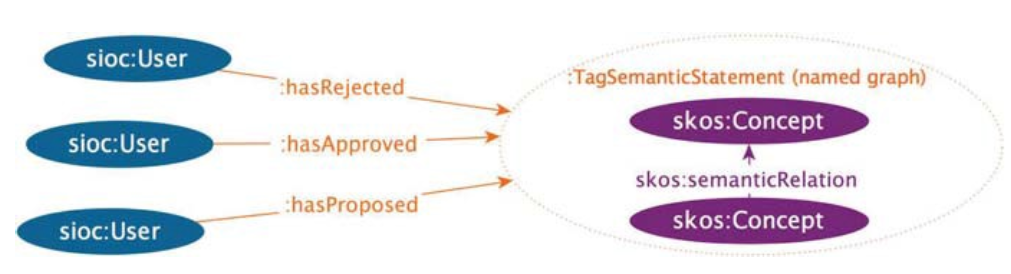
\includegraphics[width=\columnwidth]{images/SRTag.png}
\caption[SRTag RDF schema.]{SRTag RDF schema. Source: \citeonline{Limpens2013}}
\label{fig:srtag}
\end{center}
\end{figure}

\subsection{Automatic Semantic Tagging}
\label{sec:automatic_semtags}
Although this is not the main objective of this work, it is worth mentioning some strategies for automatic semantic tagging of documents.
\citeonline{Allahyari2016} proposes a probabilistic model based on DBPedia hierarchical model to automatically determine categories to documents.
The model was successfully tested on a Wikipedia sample and on a Reuters database.
Since categories are DBPedia resources, they can be considered as semantic metadata for linking purposes.

\citeonline{Chemudugunta2008} proposes a similar approach, but using unsupervised statistical learning.
The generic model can be used both with human-defined concept and data-driven topics, and was tested against an educational text corpus.

\subsection{Semantic Lifting in ODPs}
The problem of semantic lifting in ODPs was tackled by~\citeonline{Ermilov2013} and \citeonline{Ding2011}. 
In~\citeonline{Waal2014}, a strategy for lifting datasets in ODPs to the Linked Data cloud is presented. 
In all these works, however, the semantic lifting refers to the datasets, and not to metadata.

%#########################################################################################
\section{An Analysis of Metadata in ODPs}
\label{sec:analysis} 
%#########################################################################################

Besides having an overview about literature related to semantic metadata, it is also necessary to the proper development our work to profile the use of metadata in Open Data Portals.
In order to propose innovations, it is mandatory to know the main problems of real-world metadata usage.

In this section, we profile the use of metadata in Open Data Portals, with a special focus on tags. 
The analysis is restricted to systems running CKAN\footnote{Available at \url{http://ckan.org}}, the standard open-source software for ODPs. 
The CKAN community publishes a census\footnote{Available at \url{http://ckan.org/instances}}, where 139 portals were listed at the time of the experiment. 
Through the API offered by CKAN, we tried to obtain data from all portals, but only 87 responded adequately when the assessment was performed (March of 2016).
Reasons for the lack of availability were mainly that the portal was completely offline, the API was disabled or not responding at the same URL of the website or the portal was using an outdated version of CKAN.

The majority of ODPs is related to governments and public administrations at local, regional, national or continental levels. 
Some of them are also focusing on specific themes, such as energy or geothermal data. 
Although most portals are authoritative and run by governments and public administrations, some of them were built as civil society initiatives.
A complete list of the analysed ODPs is available online\footnote{\url{http://bit.ly/1NGygtk}}.

%min_datasets: 4
%max_datasets: 194592
%min_tags: 8
%max_tags: 59208
	
The analysed ODPs are quite heterogeneous. 
The number of datasets in each portals varies from 4 to 194,592, and the number of tags, from 8 to 59,208.
Regarding the quality of the portals, although there is no general benchmark, \emph{\href{http://opendatamonitor.eu}{Open Data Monitor}} attests a high heterogeneity within European ODPs.
An informal quality assessment using the Five Stars of ODPs~\cite{Colpaert2013} also shows that portals vary from simple data registries (one star) to a common data hub (five stars).

A summary of the experiment data is shown in \autoref{tab:summary}. 
The code used to collect and analyse the data is available as an open-source project\footnote{\url{https://github.com/alantygel/StodAp}}.

\begin{table}[]
\centering
\ABNTEXfontereduzida
\caption{Summary of data used in the experiment.}
\label{tab:summary}
\begin{tabular}{l|c}
Portals & 140 \\
Analysed Portals & 87 \\
Tags & 290,075 \\
Groups & 1,701 \\
Datasets & 470,551 \\
Datasets without group & 417,393 \\
Datasets without tag & 172,157 \\
\end{tabular}
\end{table}

%%\begin{savenotes}
%\begin{table}[tb]
%\caption{Summary of data used in the experiment.}
%\label{tab:summary}
%\begin{center}
%\begin{tabular}{l|c}
%Portals & 90 \\
%Datasets & 	389,913 \\
%Overall tags & 220,567 \\
%Unique tags & 148,657 \\
%Average tags per portal & 2451 \\	
%Average tags per dataset & 3.88 \\	
%Association with semantic resources & 36\% \\
%Groups & 1500 \\
%Average groups per portal\footnote{Excluding ODPs which do not use groups.} & 21.43 \\
%Average datasets per group\footnote{Excluding void groups.} & 67.45 \\
%\end{tabular}
%\end{center}
%\end{table}
%%\end{savenotes}

The analysis is divided in two groups: local metrics, to analyse the quality of tags in a particular ODP, and global metrics, looking at the interrelations between portals, and with the Linked Open Data (LOD) cloud.

Regarding the other main tool for organizing ODPs -- groups -- \autoref{tab:summary} also shows the number of groups per portal, and the number of datasets inside each one.
While the tags are attributed to an average 3.88 datasets, groups contain a mean value of 67.45 datasets.
This makes groups less selective than tags, which justifies our decision to focus on tags in this work.
Moreover, while all 87 portals use tags, 18 do not use groups to organize data.

In the following, we present the metrics and their results divided into Local Metrics, i.e., applied separately to each portal, and Global Metric, where a joint analysis is driven.
First ones aim to assess the use of tags and verify enhancement possibilities, and the last ones assess the viability of using tags as main elements of communication between portals.

\subsection{Local Metrics}
\label{sec:local_metrics}

\subsubsection{Tag Reuse}
The objective of this metric is to assess whether a single tag is being used to characterize several datasets, just a few or even only one.
Creating new tags for each dataset can be considered a bad tagging practice.
If tags are reused for several datasets, tag-based information retrieval will be more effective.
\autoref{fig:tags_once} shows the distribution of the percentage of tags used only once for each portal. 
The graphic shows a peak around 70\% of the tags used only once.
From the 87 portals, 75 use more than 50\% of the tags only once.
As a conclusion, tag reuse can be considered very low, thus effectively preventing the tags to be a suitable means to improve navigation, exploration and retrieval of datasets from ODPs.

%add examples
%include std and mean

\begin{figure}[tb]
\begin{center}
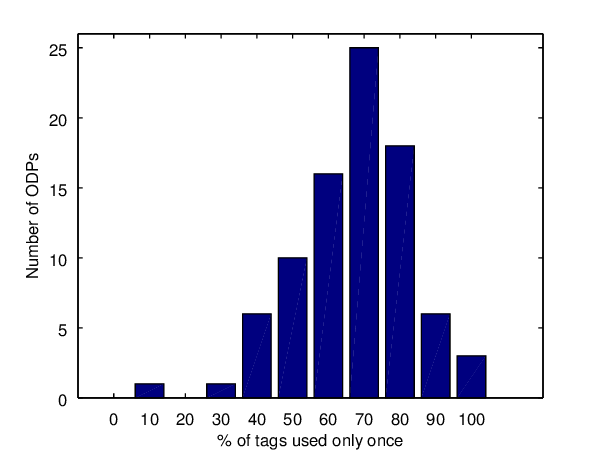
\includegraphics[width=\columnwidth]{images/tag_once_dist.png}
\caption[Re-use of tags inside an ODP.]{Re-use of tags inside an ODP. The graphic shows the distribution of the percentage of tags used only once.}
\label{fig:tags_once}
\end{center}
\end{figure}

\subsubsection{Tags per Dataset}
This metric assesses the number of tags used per dataset.
%rephrase
The goal is to verify, as in~\citeonline{Umbrich2015}, if the tag metadata is being actively used in the portals.
We must note that the results of this metric cannot lead to further conclusions, since we do not intend to define an optimal value for the number of tags per dataset. 
Using few and consistently used tags may support the organization of datasets better than many incoherently used ones.
On the other hand, few tags may not label the content adequately.
\autoref{fig:tags_per_ds} shows the distribution of the average tags per dataset for each portal. 
We can see that most ODPs apply between 1 and 7 tags to each dataset, with a peak around the value of 3.
In general, we can affirm that describing datasets with tags is a common procedure in ODPs.

\begin{figure}[tb]
\begin{center}
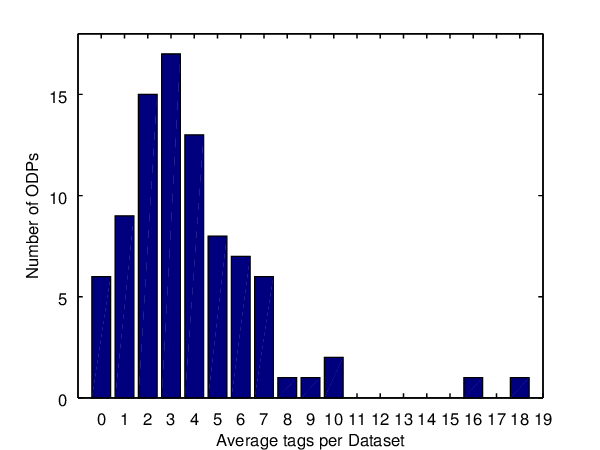
\includegraphics[width=\columnwidth]{images/tags_per_dataset.png}
\caption[Average number of tags per dataset.]{Distribution of the average number of tags used per dataset in ODPs.}
\label{fig:tags_per_ds}
\end{center}
\end{figure}

\subsubsection{Tag Similarity}
By looking at the ODP tags, one can readily recognize that many tags differ only on capitalization, accents or singular and plural forms.
Thus, this metric assesses whether several tags are being used with the same meaning.
While recognizing these cases is easy for humans who understand the language of the tags, an automatic discovery of tags with the same meaning is not always straightforward.
A simple approach is to convert the tags to lowercase and unaccented strings for comparison. 
Despite its simplicity, this method catches a significant number of cases such as \texttt{birth} and \texttt{Birth}.

A second possibility is to use the well known Levenshtein edit distance, which can also be suitable for detecting gender and plural differences, in some languages. 
This algorithm calculates the minimum number of character modifications -- insert, delete and edit -- necessary for turning a sequence into another. 
However, this method fails with tags containing numbers. 
For example, the Levenshtein edit distance between \texttt{budget-2010} and \texttt{budget-2011} is the same as between \texttt{Access} and \texttt{access}.
Semantic-oriented methods, as detailed in~\citeonline{Harispe2015}, could also be used to detect synonymous tags.

For our purposes, we define similarity as:

\begin{equation}
	S = \frac{\textrm{Similar Pairs}}{\textrm{Number of Tags}} * 100,
\end{equation}
where Similar Pairs is the number of tag pairs where tags are equal after lowercasing and unaccenting.
\autoref{fig:similarity} shows the distribution of similar tags inside each ODP.
% Similarity was checked using the simple approach.
The occurrence of a significant rate of similarity reveals that there are few portals adopting a systematic tagging procedure.
Despite the low percentage for some portals, in many of them similar tags still occur.
Only 20 portals, out of overall 87, revealed no similar tags at all. 
It should be noticed that these portals use far less tags (average 148 per portal) than the global average of 2451 per portal, which may also be a sign of careful tagging.

\begin{figure}[tb]
\begin{center}
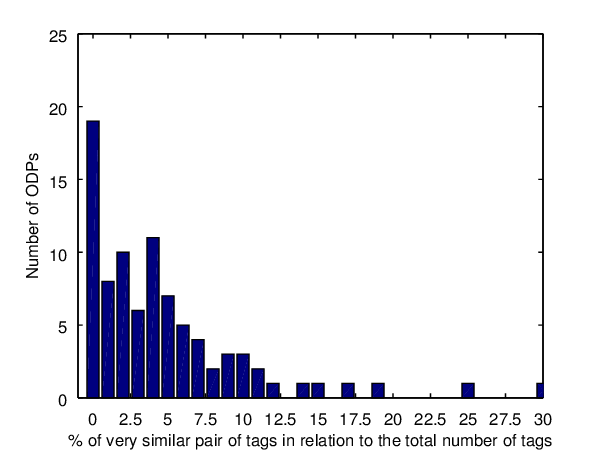
\includegraphics[scale=1.2]{images/similarity.png}
\caption[Percentage of very similar tags in ODPs.]{Percentage of very similar tags in ODPs, where the difference lies only in capitalization or special characters.}
\label{fig:similarity}
\end{center}
\end{figure}


% TODO make clear that it is only the 

\subsection{Global Metrics}
\label{sec:global_metrics}

\subsubsection{Coincident tags between portals}
Different ODPs, especially governmental ones, can publish related data, which may also be tagged similarly.
A similar measurement was used by \citeonline{Umbrich2015}.
Using the same tag comparison approach as described in the local tag similarity metric, we found that 79,882 tags appeared in more than one ODP, which represents 28\% of the total tags. 
This figure, however, should be carefully analysed. 
If we are interested in datasets from different ODPs tagged similarly, an overestimation bias may come from the fact that some portals act only as datasets harvesters, replicating the same datasets (and related tags). 
On the other hand, because portals are available in several languages, different tags could have the same meaning in different languages, what in turn tends to be an underestimation bias.
In any case, the figure clearly indicates that there exists great potential for linking tags between open data portals.
In fact, with this metric, our aim is to justify and motivate the development of a semantic tag curation approach for open data portals, which will be described in \autoref{chap:tagging}. 
%note about context: it do not make sense to compare tags between portals of different contexts
%calculate more than twice

%    Round Number: 1
%    Number of ODPs green: 87
%    Number of ODPs yellow: 1
%    Number of ODPs failled: 51
%    Number of tags: 290075
%    Number of unique tags: 210193
%    Number of datasets: 470551


\subsubsection{Tag expressiveness}
A way of taking the tagging process one step further is to associate tags with resources or terms openly described in knowledge bases.
\citeonline{Passant2008}, while building the MOAT ontology\footnote{\url{http://muto.socialtagging.org/mirror/moat.rdf}}, designed the association of tags with meanings, represented by one or more URIs in the LOD cloud.
With this expressiveness metric, our aim is to check if a tag is suitable to be connected to the LOD cloud, i.e., if there are candidate resources to represent its meaning.

Several knowledge bases are available on the Web, with DBpedia and WordNet being the most prominent ones.
They are characterized by providing both a model of data organization -- ontology -- and the individual instances.
DBpedia\footnote{\url{http://wiki.dbpedia.org/}} is build after Wikipedia knowledge base, and contains more than 38 million things, described in 125 languages using DBPedia Ontology.

WordNet \cite{Fellbaum1998} is one of the most used lexical database for the English language.
Its strengh relies on synsets describing the semantical relations between several senses of words.

In our tests for matching tags with semantic resources, we found that \url{Lexvo.org}~\cite{Melo2013}, was the better service to search connections to different semantic knowledge bases, in several languages.
Lexvo.org is connected not only to Wikipedia and WordNet, but also to Gemet, Wikitionary, Eurovoc, Agrovoc, OpenCyc and others.
By providing an isolated term (in our case, the tag) and its language, Lexvoc.org returns the corresponding translations, as \texttt{lexvo:translation}, and if the term is English, it returns semantic resources, either as \texttt{rdfs:seeAlso} or \texttt{lexvo:means}.

\autoref{tab:expressiveness} shows the results. 
The majority of tags (68.38\%) did not correspond to any semantic resource according to this method.
8.15\% of the tags were not evaluated either because they contain numbers, or because their length was equal or smaller than three. 
In those cases, results are mostly wrong.
For 23.46\% of the tags, at least one meaning or equivalent term was found, and their use represent a similar magnitude of 23.71\%.
Some tags can return several meanings, such as \texttt{leaves}\footnote{\url{http://www.lexvo.org/page/term/eng/leaves}}, for example: abandoning something, handing something to someone, or the plural of leaf, among others. 
In those cases, a further disambiguation procedure is needed.

\begin{table}[]
\centering
\caption[Expressiveness of tags.]{Expressiveness of tags. Percentage of main tags that could be associated to semantic resources. The tag universe considered here refers to clean tags, as described in \autoref{sec:local_building}, and represents 60.58\% of overall tags.}
\label{tab:expressiveness}
\begin{tabular}{|l|c|c|}
\hline
                            & \textbf{Absolute Occurrence} & \textbf{Weighted by Usage} \\ \hline
Associated to a meaning     & 26.35\%           & 36.06\%                    \\ \hline
Not associated to a meaning & 73.65\%           & 63.94\%                    \\ \hline
\end{tabular}
\end{table}

%Tags: 290093
%Main Tags: 175738
%Tags With meaning: 46317
%Tags With meaning weigted: 591429
%Tags With no meaning weigted: 1048636


It is not possible to guarantee that all associations were meaningful, and even worse, that the meaning intended by the tagger was correctly captured.
The tag language was estimated by the ODP locale metadata, which can also be a source of errors if not correctly set.
Some portals are also multi-language, and this characteristic is normally described.
Further evaluations are needed in order to estimate the potential that ODP tags have to be connected to the LOD cloud.
However, we see that at least one fifth of the tags correspond directly to a semantic resource.
Providing context and a stemming pre-processing would probably enhance this result.
Thus, we can say that some semantic potential is present on the tags.


\section{Conclusions}

In this chapter, a theoretical and practical analysis about metadata and tagging in ODPs was driven.
After a general overview on semantic tagging, a literature revision regarding metadata assessment, clean up, reconciliation and relationship presented the recent advanced of metadata curation in relation to the Semantic Web tendency.

Apart from the literature review, looking at the actual use of tags in ODPs was also necessary.
An analysis of 87 ODPs revealed that: (i) tags in ODPs are widely used, but in a non-systematic way, which hinders their capacity of supporting information retrieval, and (ii) there is a potential for using these tags as connecting elements between ODPs, and for raising semantics from them.
Next, we describe our proposal based on these statements.

Ideas and gaps noticed on the literature, and actual problems and potentials detected on ODPs are the basis for proposing the STODaP approach that will be described in the following chapter.

%metadado, extração, muito breve, uma vez tendo tags, o que eu faço para melhorar
%bernardo azevedo tentando pegar localização de tweets - "teoria da mutua informação", tentando descobrir o que está fortemente relacionado e o que não está relacionado. Bons resultados
% tem que ir afunilando para semantica


%% justificativa do capitulo 3: abordagem semi-automatica, puxando para o lado da colaboração
%% imaginar que o processo da descoberta de links tem uma parte automática, mas uma parte de participação dos usuários.
%% viu bastante isso em trabalhos recentes, um deles foi o projeto final da karen na parte de extração semântica de texto, extraindo relações da wikipedia. dado que a dbpedia so pega relações do box, foram para o texto e tentaram extrair e selecionar fatos sobre esse objeto, para complementar a dbpedia . 
%% extração de ontologia a partir do texto, tira as triplas do texto e pede para um usuário validar.
%% joao trabalho bem na parte da relações - 1o identifica as entidades

%% dado que eu to tentando entender, será que eu consigo ter uma mediação para enriquecer com feedback do humano, tanto com especiliastas de domínio qto com usuários

%% usar os usuários na validação do que é automático!!!

%já tentaram descrever melhor, assim assim assado - e os gaps
%(metadata) semantic enrichment 

%Mutual information - o que é mais significativo em um grupamento, que o faz diferente do outro - explorar ligações entre elementos 

%qual a relação do datasem a tag?


\chapter{Semantic Tags for Open Data Portals}
\label{chap:tagging}


As observed in the previous chapter, literature related to semantic enhancement of ODPs metadata has still some significant gaps, such as:
\begin{itemize}
	\item Emerging semantics from the ODP context;
	\item Dealing with multiple languages;
	\item Tags attributed by few users, in a non-folksonomy style;
	\item Integrating multiple domains.
\end{itemize}

In order to	tackle this issue, we describe in this chapter the Semantic Tags for Open Data Portals - STODaP approach for improving tag curation within and across ODPs, and for linking ODPs through its metadata.

Besides the comprehensive analysis of tag usage in 87 ODPs, shown in previous chapter, that justifies the need and benefits of better tools for managing tags, our main contributions are:
\begin{itemize}
	\item An approach for cleaning and reconciliation of metadata in ODPs;
	\item An approach for semantic lifting of metadata in ODPs;
	\item A centralized repository for connecting ODPs through meaningful shared tags.
\end{itemize}

%TODO: organize
This chapter begins with a short motivation to our work, which is also justified by the previous chapters.
In the first section, some considerations about metadata in open data portals are derived. 
In the following, the different concepts of tagging are put into perspective, in order to characterize tags in ODPs. 
Section~\ref{sec:analysis} presents an analysis of the use of tags in several Open Data Portals, both from government and civil society side, and from various countries and languages.
The main part of this chapter lies in Section~\ref{sec:stodap_architecture}, where our approach for semantic tags in open data portals is explained. 
Following sections presents some aspects about the implementation, the validation of the approach, and a conclusion.

%#########################################################################################
\section{Motivation}
%#########################################################################################

Analysing large amounts of data plays an increasingly important role in today's society. 
However, new discoveries and insights can only be attained by integrating information from dispersed sources. 
Despite recent advances in structured data publishing on the Web (such as RDFa and the schema.org initiative) the question arises how larger datasets can be published and described in order to make them easily discoverable and facilitate the integration as well as analysis.

One approach for addressing the problem of data dispersion are data catalogues, which enable organizations to upload and describe datasets using comprehensive metadata schemes. 
Similar to digital libraries, networks of such catalogues can support the description, archiving and discovery of datasets on the Web. 
Recently, we have seen a rapid growth of data catalogues being made available to the public. 
The data catalogue registry \href{http://datacatalogs.org}{datacatalogs.org}, for example, already lists 285 data catalogues worldwide. 

Data catalogues where data is supposed to be open, at least in the licensing sense, are usually called Open Data Portals (ODPs).
Implementations that show the increasing popularity of ODPs can be seen, for example, in open government data portals, data portals of international organizations and NGOs, as well as scientific data portals.

In order to increase transparency and citizen engagement, governments and public administrations all over the world are implementing ODPs. 
These ODPs comprise large amounts of structured data, mostly in the form of tabular data such as CSV files or Excel sheets. 
They aim to be a one-stop-shop for citizens and companies interested in using public data produced by governments or civil society organisations.
Examples are the \href{http://data.gov}{US' data portal}, the \href{http://data.gov.uk}{UK's data portal}, the \href{http://open-data.europa.eu}{European Commission's} portal as well as numerous other local, regional and national data portal initiatives.

In the research domain ODPs also play an important role.
Almost every researcher works with data. 
However, quite often only the results of analysing the data are published and archived. 
The original data, that is ground truth, is often not publicly available thus hindering repeatability, reuse as well as repurposing and consequently preventing science to be as efficient, transparent and effective as it could be. 
An example of a popular scientific open data portals is the \href{http://data.gbif.org}{Global Biodiversity Information Facility Data Portal}.
Also many international and non-governmental organizations operate ODPs such as the \href{http://data.worldbank.org}{World Bank Data Portal} or the data portal of the \href{http://apps.who.int/gho/data/}{World Health Organization}.
Although being a relatively new type of information system first commercial (e.g. Socrata) and open-source (e.g. CKAN) data portal implementations are already available.

Despite its recent popularity, Open Data and Open Data Portals still face significant impediments, as richly described in Section~\ref{sec:problems}.
Authors collected 118 socio-technical impediments for use of open data from interviews, workshops and literature.
Some cited impediments were ``absence of commonly agreed metadata'', ``insufficiency of metadata'', ``the lack of interoperability'' and ``difficulty in searching and browsing data'', showing that a great challenge for ODPs is the organization of data.

The open data organization challenge can be subdivided into two aspects: 1) structuring and organizing the datasets themselves and 2) providing well-structured and organized metadata for the datasets.
The first aspect was, for example, tackled by approaches for semantic lifting of data by~\cite{DBLP:conf/i-semantics/ErmilovAS13} and~\cite{Ding2011325}, who tried to build general strategies for putting large open government datasets in the Link Data cloud.
For the standardized structuring metadata, the Data Catalog Vocabulary (DCAT)\footnote{Available at \url{http://www.w3.org/TR/vocab-dcat/}}~\cite{conf/i-semantics/CyganiakMP10} was developed.
However, the cross-portal metadata alignment and reconciliation can not be addressed by DCAT.

The metadata used to organize datasets in an ODP comprises categories or groups and most importantly labelling with free-text words or sets of words -- the tags.
The concept of tagging became popular within Web 2.0 services and aggregation tools like del.icio.us. 
The main advantages of tagging are the ease of classifying, and the crowd effect -- resulting in the so called folksonomies -- because all users were allowed to tag and share their contents. 
Tagging datasets in an ODP cannot be considered as folksonomies, because the process is mainly driven by portal managers and data publishers, and not by the actual users.
As a result of this, the structuring effect of crowd-tagging and folksonomies is missing in ODPs.

A quick look over some ODPs reveals that most of them suffer from a very confusing organization of datasets. 
The first level of categorization uses the concept of groups.
In general, they are stable and meaningful, but normally contain a large number of datasets.
A more detailed classification should be done via tags, whose use in ODPs has the following issues:

\begin{itemize}
	\item \emph{Synonyms:} In most ODPs, there exists large number of synonymous tags, e.g., \texttt{crops} and \texttt{seeds};
	\item \emph{Different spellings of the same word:} Several tags are incorrectly written, or have differences in capitalization or accents, e.g., \texttt{baden-wuerttemberg} and \texttt{Baden-W\"{u}rttemberg};
	\item \emph{Lack of relationships:} There is no explicit relationships between the tags, e.g., \texttt{Community Centres} is clearly a specialization of \texttt{Community}, but this is not explicit;
	\item \emph{Ambiguity:} As tags are written as pure text, ambiguity is prevalent in ODPs, e.g., the tag \texttt{apple}, which could refer to the fruit or to the company; and
	\item \emph{Incoherence:} Tags do not allow any connection between different portals that use the same or equivalent tags, e.g., two datasets tagged with \texttt{budget} in different portals are not connected.
\end{itemize}

As a result, the navigation, exploration and search within individual, but in particular also across ODPs is significantly hampered.
Thus, we present in the following the STODaP architecture, whose intention is to facilitate access to data.


%#########################################################################################
\section{The STODaP Architecture}
\label{sec:stodap_architecture}
%#########################################################################################

In this section, we present the tag reconciliation approach for cleaning up and connecting ODPs, supported by software tools both at the local and global contexts.
The objective of this approach is to tackle the main problems identified by the metrics described in \autoref{sec:analysis}, and thus to facilitate data organization and linking through metadata descriptions of ODPs.

Figure \ref{fig:overview}\footnote{Icons by \href{http://www.flaticon.com/authors/simpleicon}{SimpleIcon} from \href{http://www.flaticon.com}{www.flaticon.com} are licensed under \href{http://creativecommons.org/licenses/by/3.0/}{CC BY 3.0}.} shows an overview of the proposed approach.
Data publishers in charge of ODPs are offered tools for enhancing local tag curation and semantic lifting.
These local tags are then connected to semantic tags hosted in a central server, which is automatically fed by data coming from ODPs.
% They can add new semantic descriptions to the global tags, establish relations between them, and also create new links between global and local tags.
Data consumers have the option to retrieve data directly from ODPs, or through references gathered from the central server.
%The description of these actions is shown in the sequel.

\begin{figure*}[t]
\begin{center}
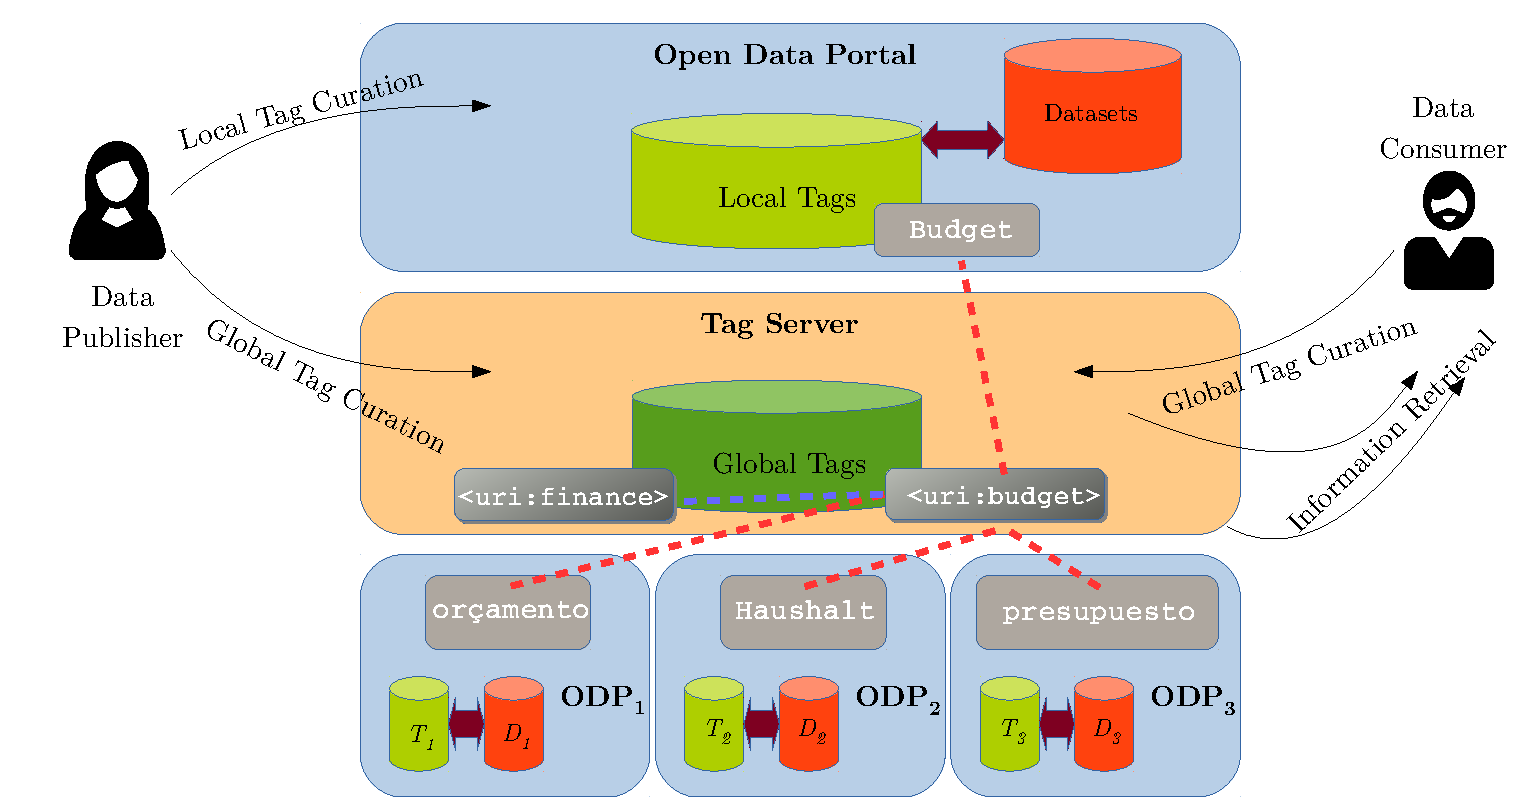
\includegraphics[width=\columnwidth]{images/overview.pdf}
\caption[Overview of the STODaP approach.]{Overview of the STODaP approach. Local tags are connected to a corresponding semantic tag within a central tag server. 
Data managers responsible for ODPs may use tools for local tag curation and semantic lifting of metadata.}
\label{fig:overview}
\end{center}
\end{figure*}

This section is divided as follows: first, we present an overview of the STODaP architecture in \autoref{sec:stodap_architecture_overview}.
The following subsections describe each element of this architecture, specifically the Open Data Portals (\autoref{sec:definition}), the Local and Global Processing steps (\autoref{sec:local_building} and \ref{sec:global_building}), the STODaP vocabulary (\autoref{sec:stodap_vocabulary}), the external plugins (\autoref{sec:tag_manager_plugin} and \autoref{sec:semantic_tags_plugin}) and the external query interfaces.


%#########################################################################################
\subsection{Architecture Overview}
\label{sec:stodap_architecture_overview}
%#########################################################################################

\begin{figure*}%[tb]
\begin{center}
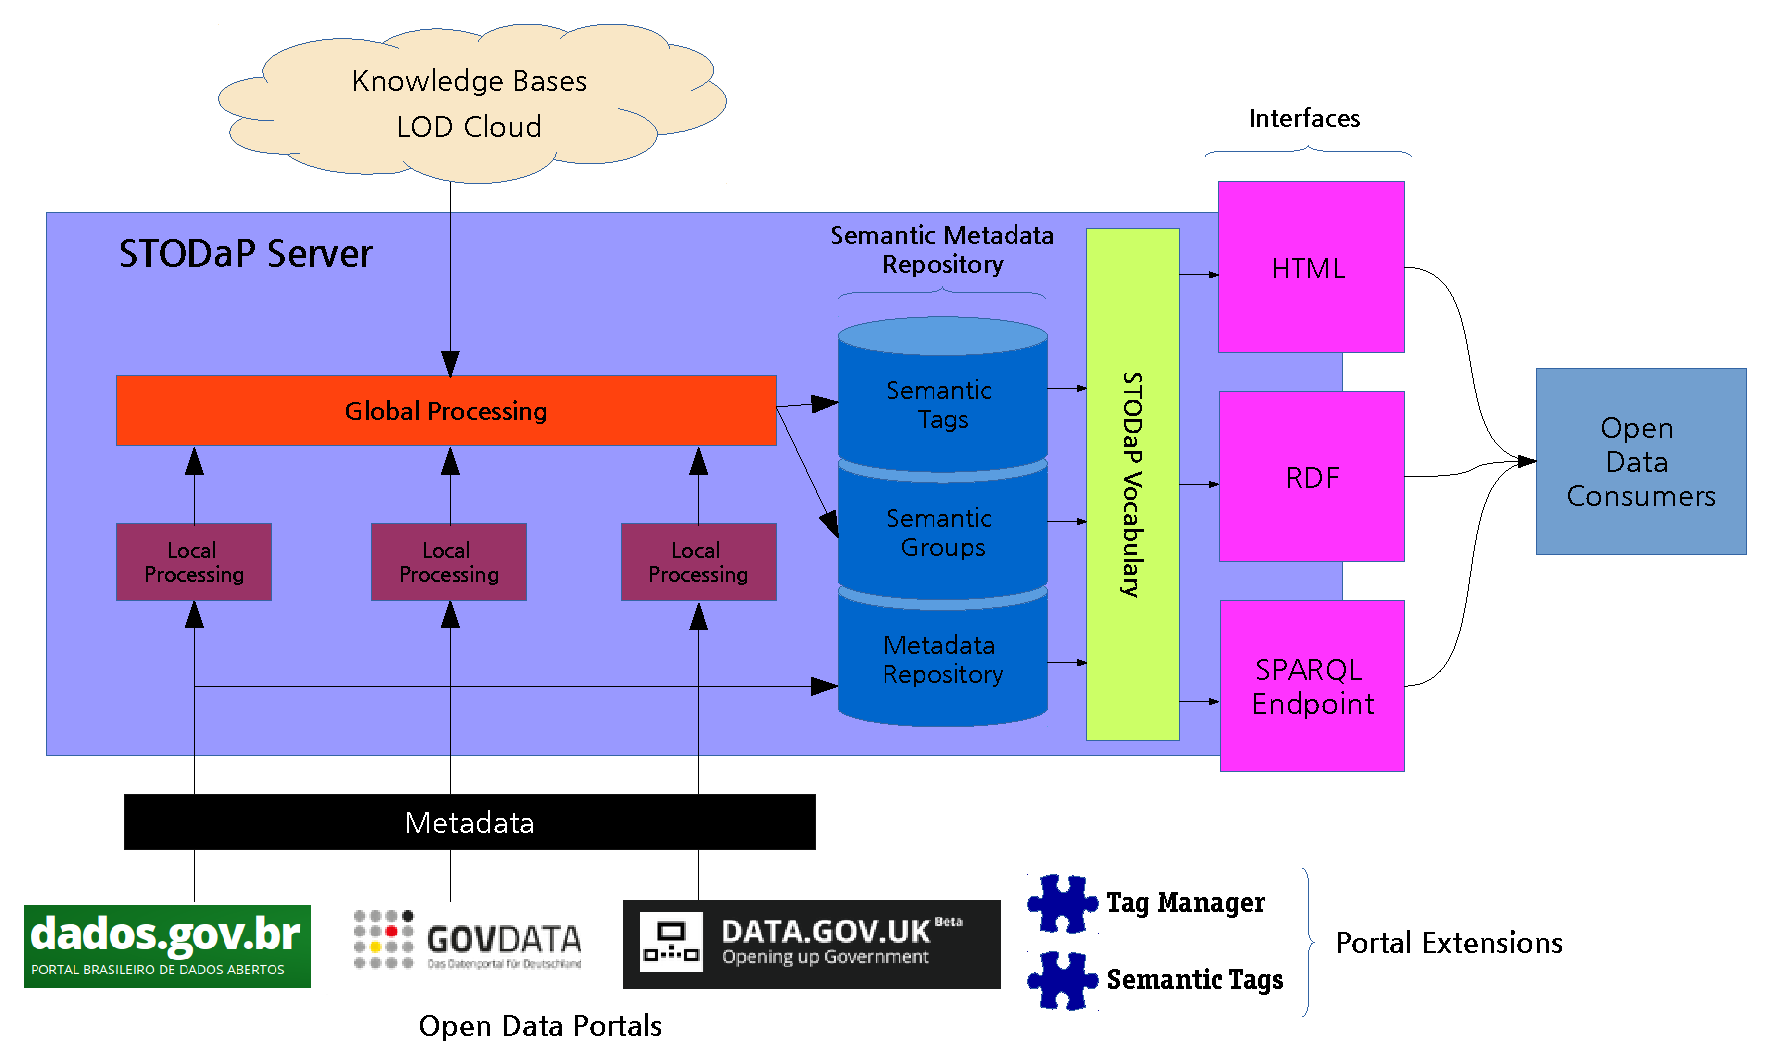
\includegraphics[width=\columnwidth]{images/architecture.pdf}
\caption[Architecture of the STODaP approach.]{Architecture of the STODaP approach.}
\label{fig:architecture}
\end{center}
\end{figure*}

\autoref{fig:architecture} depicts the architecture of STODaP approach.
The system receives as main input metadata of Open Data Portals, which are basically dataset descriptors such as title, description, tags, themes and others.
These metadata is pre-processed individually for each portal at the Local Processing phase, and stored at the Metadata Repository..
Metadata is also jointly processed, together with data coming from semantic knowledge bases from the Linked Open Data cloud, at the Global Processing phase.
This phase results in the Semantic Tags and Groups, which are then coded using the STODaP vocabulary.
Resultant dataset is made available for the general public through three types of interface: an HTML website where users can navigate manually, an RDF/XML interface which responds to machine requests searching for the resources URIs, and a SPARQL endpoint which accepts queries and responds with JSON coded triples.
In addition, the STODaP also offer plugins for ODPs for enhancing tag management and for linking tags with the server.
The STODaP approach is independent of these plugins, and their implementation is under control of portal administrators.

In the following, each of these blocks is explained in details.

%#########################################################################################
\subsection{Open Data Portals}
\label{sec:definition} 
%#########################################################################################

According to~\citeonline{Colpaert2013}, an Open Data Portal is ``a collection of systems set up to make Open Data used and useful''.
% This definition sounds quite ambitious, since the great majority of ODPs are not a collection of systems, but of datasets.
A formal definition of an ODP can be found in~\citeonline{Umbrich2015}.
However, in that case, the focus is general metadata analysis, which turns their definition unsuitable to be used here. 
In this section, we will describe the elements that are present in the context of this work.

Figure \ref{fig:definition} shows the relevant entities and relations that are used in the remainder of this paper.
An \emph{Open Data Portal}, in this context, is a collection of datasets, which hold open data resources online.
\emph{Datasets} can be organized in \emph{Groups}.
Each \emph{Dataset} belonging to an ODP can be tagged with local tags. 
Each \emph{Local Tag} also belongs to an ODP, and can be used to tag one or more datasets.
In this architecture, local tags are connected to \emph{Semantic Tags}, stored in a collaborative \emph{Tag Server}.
Several local tags from different ODPs can be associated to a single semantic tag, which can also have semantic relationships with other semantic tags.

\begin{figure}
\begin{center}
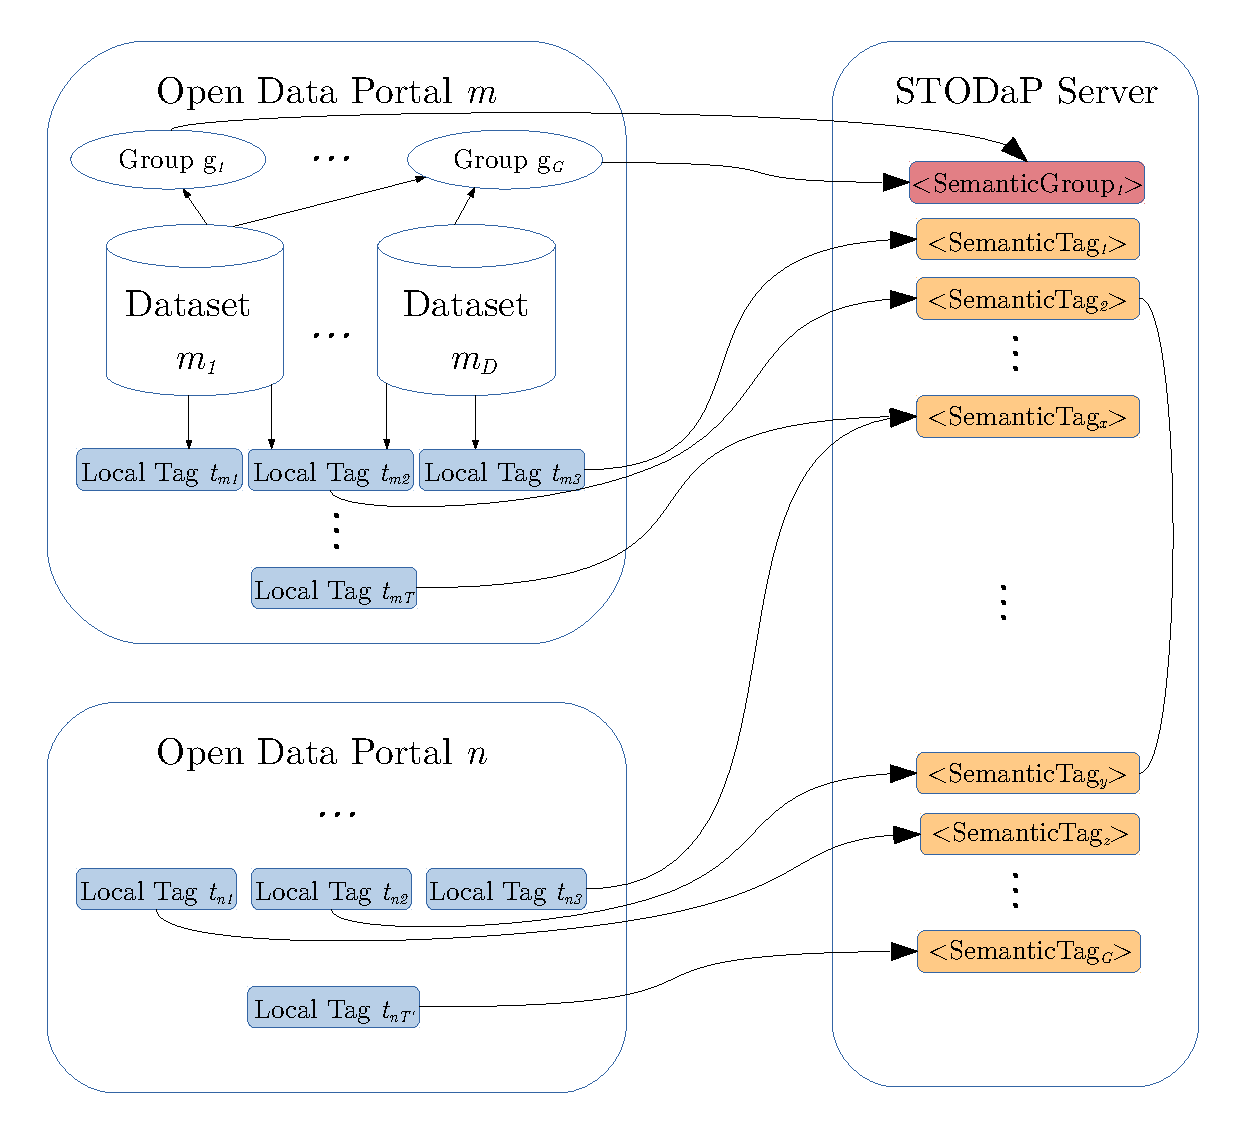
\includegraphics[width=\columnwidth]{images/odp_definition.pdf}
\caption{Relevant elements of the Semantic Tags for Open Data Portals system.}
\label{fig:definition}
\end{center}
\end{figure}


%##################################################################
\subsection{Local Processing - Clean Up and Reconcile}
\label{sec:local_building}
%##################################################################

In order to build the first version of the STODaP server, a metadata harvesting was driven through 87 ODPs.
Almost 500.000 datasets were processed, using their metadata such as names, language, tags and groups they belong to.
In the following, we describe the procedures applied to the individual portals, in the process called Local Processing, which refers to the fact that it deals only with individual ODPs data.

An overview of the procedure applied for each ODP is shown in \autoref{fig:local_processing}.
In the figure, each green block represents a processing phase, which is materialised in a set of tag representations. 
The grey blocks describe the transformations suffered by the tag sets from one phase to another.
The aim of the local processing steps is to transform freely written tags into semantic resources that are candidates for representing the datasets they are associated.
Each transformation applied to the tags on the local processing is detailed bellow:

\begin{figure*}[tb]
\begin{center}
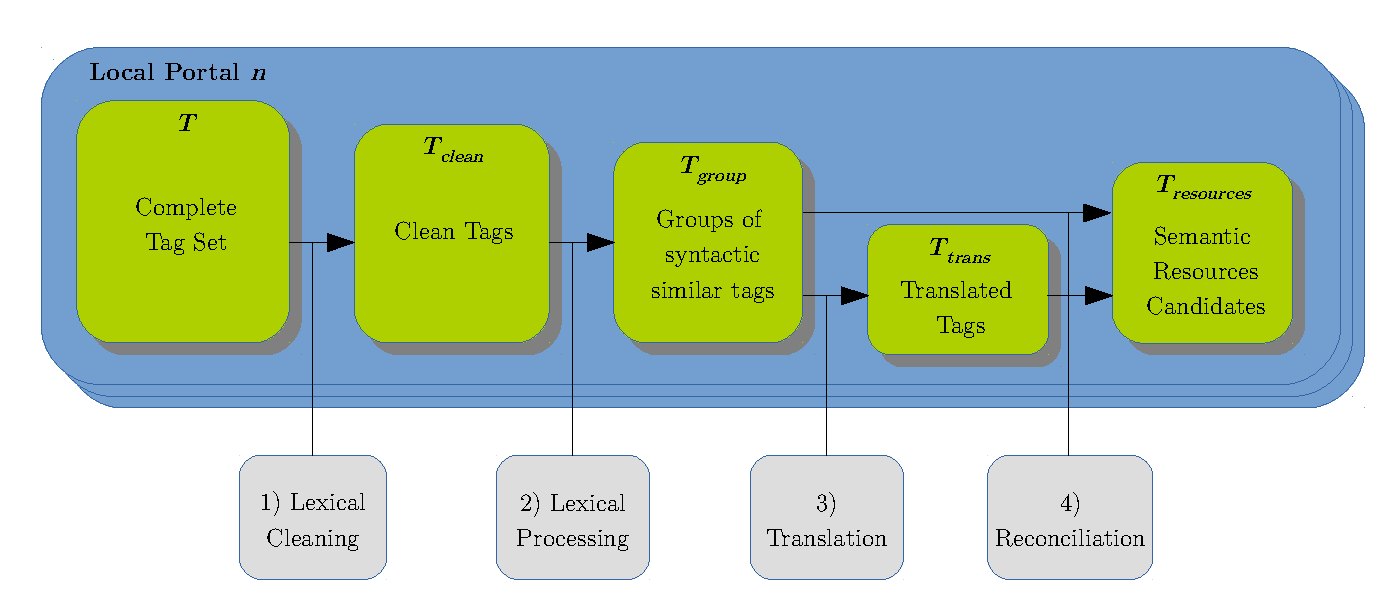
\includegraphics[width=\columnwidth]{images/local_processing.pdf}
\caption[Overview of the local tag processing.]{Overview of the local tag processing.}
\label{fig:local_processing}
\end{center}
\end{figure*}

\noindent \textbf{Lexical Cleaning: }The complete tag set $T$ is the set containing all original tags found in one portal.
Firstly, the \emph{Lexical Cleaning} is applied in order to discard tags with low probability of getting a semantic meaning.
At this point, some heuristics are applied, and a tag is discarded if it is: 
\begin{itemize}
	\item smaller than 4 characters; 
	\item composed of numbers and alphabetic characters;
	\item exclusively composed by uppercase characters;
	\item not started by a alphanumerical character;
	\item larger than 5 words; or
	\item not applied to any dataset.
\end{itemize}

\noindent \textbf{Lexical Processing:} After the Lexical Cleaning, we have the resulting set $T_{clean}$ of clean tags, with a higher probability of being reconciled with semantic concepts in ontologies.
The following procedure is the \emph{Lexical Processing}, which aims to group tags that have a lexical similarity.
These similar tags have a high probability of representing the same meaning, with small lexical variations.
In order to determine this similarity, we apply the Levenshtein edit-distance to the lowercased and unaccented tags (which means that \texttt{Açaí} will be transformed into \texttt{acai} before measuring the distance).
Based on manual experimentation, we consider that tags with an edit-distance of 0 or 1 are similar.
This distance captures plural, gender and temporal variations in most of the languages present in our sample.
The proceeding results in the set $T_{group}$ of syntactically similar tags.

\noindent \textbf{Translation:} The sample used to build this tag server contains portals in 22 different languages.
Thus, it is necessary to use translation services on the Web to transform words from their original language to the English language.
English language was chosen because of the higher availability of translation services, and also because the main ontologies have their terms described necessarily in English, and possibly also in other languages.
It also significant that 43\% of the portals are in English (according to the provided metadata), and their tags represent 83\% of all tags.
Each group of similar tags from $T_{group}$ was translated, resulting possibly in a set of translations for each group.
The new set achieved in this processing is $T_{trans}$.

\noindent \textbf{Reconciliation:} The previous proceeding results in a set $T_{trans}$ of groups formed by all the related translations.
Until this moment, we were dealing with string of characters.
In this stage, these names will be the input for searching semantic representations for the tags.
In order to get the widest spectrum of possibilities, the search for semantic resources is done for all lexical representations of the tag, stored in $T_{group}$, and also all possible translations of it in $T_{trans}$.
The resulting set will be denominated $T_{resources}$.

%The product of this step are synonym rings, or synsets, where the groups of words have are semantically equivalent for the purpose of retrieving information.
%The proceeding results in the set $T_{synt\_sem}$ of semantically similar tags.

%Finally, in order to prepare the tags for linking with other portals, we come to the \emph{Translation} step.
%Each tag is translated to the English language, forming the set $T_{english}$ of translated tags.
%->> tentar todas as opções de tradução
In order to illustrate the procedure, \autoref{tab:local_example} shows an example using real tags from the Brazilian Data.gov.br.
From $T$ to $T_{clean}$, tags containing numbers, too small or representing abbreviations were removed.
Then, similar tags were grouped to form $T_{group}$.
The translation process could not find an equivalent for the first group.
Even so, the semantic search-engine was able to find a matching resource for \texttt{Acidente de trabalho} (accident at work), as well as for the other two.

\begin{table}[]
\centering
\ABNTEXfontereduzida
\caption{Examples of tags in each step of the procedure.}
\label{tab:local_example}
\begin{tabular}{|p{2cm}|p{2cm}|p{2cm}|p{2cm}|p{2cm}|p{2cm}|}
\hline
$T$ & $T_{clean}$ & $T_{group}$ & $T_{trans}$ & $T_{resources}$ \\ \hline
Acidente de trabalho,
Acidentes de trabalho,
CNAE,
finanças,
Folha SA.23,
Folha SB.23 
município,
orçamento,
UF
&
Acidente de trabalho,
Acidentes de trabalho,
finanças,
orçamento
&
\{Acidente de trabalho, Acidentes de trabalho\}
finanças,
orçamento
&
--
finances,
budget
&
\{gemet:9366, eurovoc:825\},
eionet:3194
eionet:1025 \\ \hline
\end{tabular}
\end{table}

It is important to notice that the process described above is subject to several failures.
On the Lexical Cleaning step, meaningful tags with less than 4 characters may be discarded, as well as unintentionally uppercased words.
On the Lexical Processing stage, it is possible that in some languages the same word starting with capital and non-capital letters have different meanings.
With a higher probability, words differing from edit-distance of 2 may also have different (or even opposed) meanings, such as \texttt{child-death} and \texttt{child-health}, found on data.gov.uk.
On the Translation phase, the main problem lies on polysemy, where the same word has several meanings.
While also heavily dependent on the translation tools, providing side tags or other metadata can help the algorithm finding the right translation.
Finally, when searching for the meanings, there is a great dependency on the tool used and the available knowledge bases.

%#######################################################################
\subsection{Global Processing - Interlinking Portals}
\label{sec:global_building}
%#######################################################################

After reaching the last stage of the local processing stage for each one of the 87 portals, a joint process starts over $T_{resources}$ in order to build the Semantic Tag Server.
At the global processing stage, there are three main steps:

\begin{enumerate}
	\item Select meaningful tags;
	\item Create semantic tags and connect local tags to them; and
	\item Discover and qualify relations between tags.
\end{enumerate}

In order to accomplish this objective, we propose the global procedure shown in Figure~\ref{fig:global_processing}.

\begin{figure*}[tb]
\begin{center}
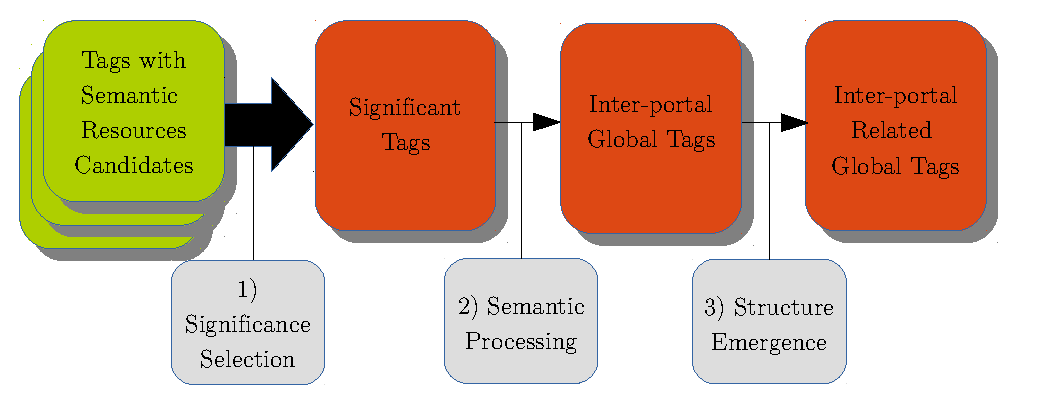
\includegraphics[width=\columnwidth]{images/global_processing.pdf}
\caption[Overview of the global processing.]{Overview of the global processing.}
\label{fig:global_processing}
\end{center}
\end{figure*}

\noindent \textbf{Significance Selection: } We start the global processing with a joint set $\mathcal{T}_{resources}$, which contains $T_{resources}$ from all portals. 
In this set, a \emph{Significance Selection} process is driven, in order to determine tags that will be useful on the information retrieval process.
This is an heuristics based process, which considers: (i) Success on finding semantic candidates for the tag; (ii) the number of datasets pointed by this tags; (iii) the quality of the semantic resources candidates.

\noindent \textbf{Semantic Processing:} After this step, the Semantic Tags will be derived.
Semantic Tags are entities on the web, who have a main name in English, several translations, and point to local tags, which in turn connect to datasets located into Open Data Portals.

\noindent \textbf{Structure Emergence:} Finally, relations between Semantic Tags in set $G$ will be searched on the ontologies they appear in order give a structure to the Semantic Tag set $G_{struct}$.
The first strategy is to search for relations on the reconciled ontologies, and set this relation between the semantic tags.
Thus, relations as \texttt{skos:related}, \texttt{skos:narrower} and \texttt{skos:broader} can be set.
However, at this point we notice need of an upper classification scheme.

The ODP model, as shown in \autoref{fig:definition}, includes a Group element, to which one or more datasets can be associated.
Thus, it is possible to consider that a tag associated to a dataset which is in a group is also related to this group.
However, only 11\% of all datasets in our sample are associated to groups, and only 13\% of the tags are associated to datasets in groups.

If we look to some ODPs which are organized in groups, it is possible to see a similar organization.
In \autoref{tab:groups}, we list the groups of 4 ODPs. 
If we look at the table, it is clear that in the context of open government data portals, there are some specific categories, but the portals also share common subjects, such as Health, Education or Culture.

\begin{table}[]
\centering
\ABNTEXfontereduzida
\caption{Examples of groups in some ODPs}
\label{tab:groups}
\begin{tabular}{|p{3.2cm}|p{3.2cm}|p{3.2cm}|p{3.4cm}|}
\hline
Data.gov & Data.gov.de & Dados.gov.br & Data.buenosaires.gob.ar \\ \hline
Aging / Agriculture / Business / Climate / Consumer / Disasters / Ecosystems / Education / Energy / Finance / Health / Law / Local Government / Manufacturing / Ocean / Public Safety / Science \& Research &
Population / Education and science / Geography, Geology and the GEODATA / Laws and justice / Health / Infrastructure, building and housing / Culture, leisure, sport, tourism / Not yet categorized / Public administration, budget and taxes / Politics and elections / Social / Transport and traffic / Environment and the climate / Consumer protection / Economy and work &
Municipal Chamber
/ trade, services and tourism
/ culture, leisure and sport
/ data sets in the spotlight
/ defence and security
/ economy and finance
/ education
/ public facilities
/ geography
/ government and politics
/ housing, sanitation and urbanism
/ health information
/ industry
/ justice and law
/ environment
/ person, family and society
/ management platform indicators
/ multi-year plan
/ international relations
/ health
/ work
/ transportation and transit &
economic activity /
public administration and policy /
culture and recreation /
education /
infrastructure and public works /
environment /
mobility and transport /
health and social services /
security /
urbanism and territory \\\hline
\end{tabular}
\end{table}

Thus, after translating all the group names, we verified that 62 group names occurred in three or more portals.
These were chosen as the first Global Groups.
The second step consisted in verifying the lexical similarity between all groups and the Global Groups in order to associate groups with Global Groups.
Some distortions were observed, such as \texttt{sport} being associated with \texttt{transport}, or \texttt{culture} with \texttt{agriculture}.
These errors were manually corrected.

Finally, groups were reconciled with general-purpose ontologies.
Particularly, the Gemet Thesaurus\footnote{Available at \url{http://www.eionet.europa.eu/gemet/}} fits well for this purpose.

%All Datasets: 470551
%Datasets in Groups: 53158
%Tags in Groups: 37743

%#######################################################################
\subsection{Semantic Metadata Repository}
\label{sec:semantic_tags_plugin}
%#######################################################################

With the aim of building a common basis for interlinking ODPs, we developed a Semantic Metadata Server.
The conceptual rationale is:
\begin{enumerate}
	\item To assist individual ODPs enhancing the quality of their tags, by assigning a common agreed meaning to them;
	\item To create a collaborative platform for meaningfully linking ODPs.
\end{enumerate}

The Semantic Metadata Server hosts the description of semantic tags and groups.
Each semantic tag may be associated to one or more Linked Open Data resources, representing their semantic meanings.
Linking to the local tags is accomplished via the URIs which represent a local tag in its context.
The semantic tags can also have several types of relations between each other, such as \texttt{skos:broader}, \texttt{skos:narrower} or \texttt{owl:sameAs}.
Figure \ref{fig:example} illustrates the concept with an example.

\begin{figure}[tb]
\begin{center}
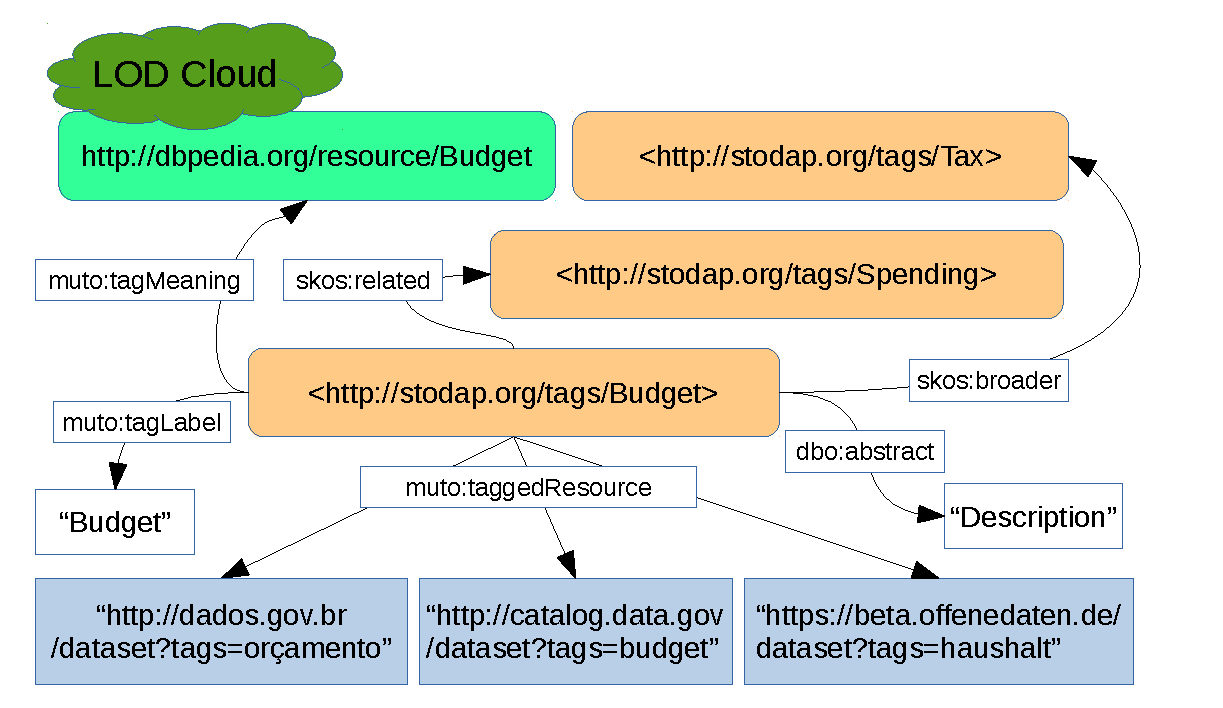
\includegraphics[width=\columnwidth]{images/example.pdf}
\caption[Example of the STODaP model.]{Example of the STODaP model showing relationships of the semantic tag \url{http://stodap.org/tags/Budget}.}
\label{fig:example}
\end{center}
\end{figure}

The example shows the semantic tag identified by the URI \texttt{<http://stodap.org/tags/Budget>}. 
With this semantic tag, a meaning and some URIs of local tags are associated.
The semantic tag is also semantically related to other semantic tags, using the SKOS vocabulary.
The MUTO ontology\footnote{\url{http://muto.socialtagging.org/core/v1.html}} is used to define some concepts and relations between the tags, like \texttt{muto:Tag}, \texttt{muto:taggedResource}, \texttt{muto:hasTag} and \texttt{muto:hasMeaning}.

%#######################################################################
\subsection{STODaP Vocabulary}
\label{sec:stodap_vocabulary}
%#######################################################################

\begin{figure*}[b]
\begin{center}
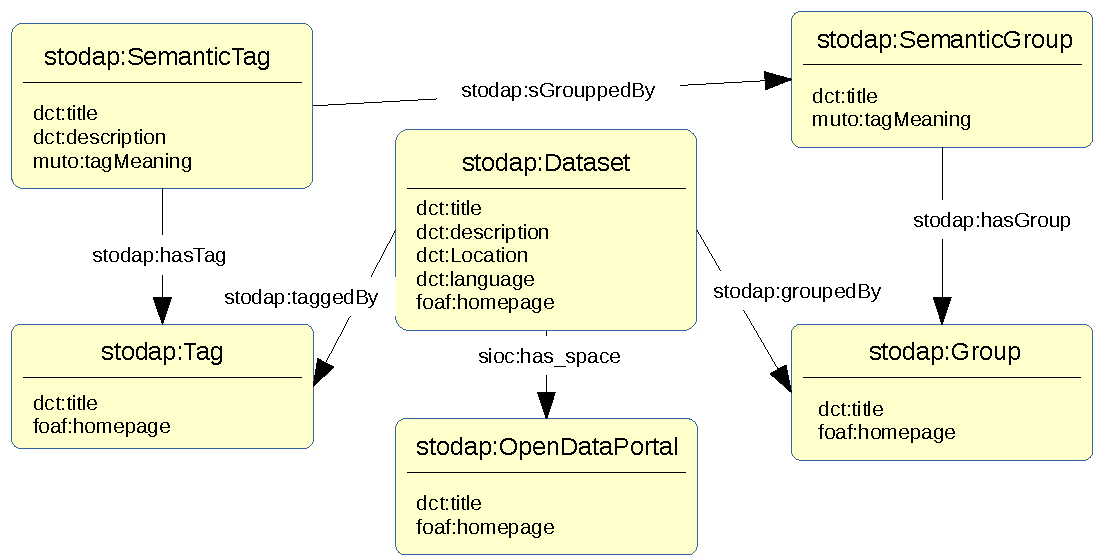
\includegraphics[width=\columnwidth]{images/stodap_vocabulary.pdf}
\caption[Simplified schema of the STODaP vocabulary.]{Simplified schema of the STODaP vocabulary. Some elements are equivalent to other vocabularies and ontologies, such as SIOC, DCAT and MUTO.}
\label{fig:vocabulary}
\end{center}
\end{figure*}

In order to represent data in our system, it was necessary to create a simple vocabulary.
\autoref{fig:vocabulary} shows a simplified schema of the STODaP vocabulary.
As shown in \autoref{sec:semantic_metadata}, several works describe ontologies and vocabularies related to our work.
However, it was not possible to fit all entities of STODaP architecture on existing ontologies.
Specifically, DCAT\footnote{Available at \url{http://www.w3.org/ns/dcat}.} defines some important entities, such as \texttt{dcat:Dataset} and \texttt{dcat:Catalog}.
They are defined as equivalent (\texttt{owl:equivalentClass}) to \texttt{stodap:Dataset} and \texttt{dcat:Catalog}, respectively.
At DCAT, tags are represented as literals, which means that two tags with the same label do not differ.
This is not the case at STODaP, where each tag is an entity.
MUTO\footnote{Available at \url{http://muto.socialtagging.org/}.} tackles this issue with the class \texttt{muto:Tag}, equivalent to our \texttt{stodap:Tag}.
On the semantic side, MUTO systematized the relation between a tag and a meaning with the \texttt{muto:tagMeaning} property.
Thus, although some concepts were reused, \texttt{stodap:SemanticTag} and \texttt{stodap:SemanticGroup} needed to be defined.
It must also be noted that MUTO works with a social concept of tagging, and thus defines a \texttt{muto:Tagging} class to enable relating actor to a tagging event, as described by~\citeonline{Grubber2007}.
Since the Open Government Data domain is not social, at least in the sense of tagging, this was not necessary in our case.

\noindent \textbf{\texttt{stodap:SemanticTag}:} A Semantic Tag is a super tag that groups open data portal tags and is connected to a semantic resource on the Linked Open Data Cloud.

\noindent \textbf{\texttt{stodap:SemanticGroup}:} A stodap:SemanticGroup is a super group of tags that groups open data portal groups, open data portal tags, and semantic tags. It is connected to a semantic resource on the Linked Open Data Cloud.


\subsection{Cleaning up and semantifying tags}
\label{sec:tag_manager_plugin}

Section \ref{sec:local_metrics} showed that ODPs suffer from low reuse of tags, and that there is a significant tags duplication due to slight spelling differences. 
In fact, both problems -- low reuse and duplication -- are connected, since merging similar tags improves tag reuse.
However, low tag reuse can be also attributed to the lack absence of a standard tagging procedure, which would guide users in this task.

To address this problem locally at a particular ODP, we propose an approach for clean-up and reconciliation of tags. %, and for enhancing the quality of the new ones.

First, we offer three levels of semi-automatic tag merging strategies:

% spell 
% check for sem similatyy libs in phyton

\begin{enumerate}
	\item With high confidence, we suggest merging tags that differ only by capital letters or special characters. 
In many ODPs, this strategy will already achieve significant results, as shown in Figure~\ref{fig:similarity}.
	\item After running the first strategy, the Levenshtein distance is computed for all remaining pairs of tags.
Tags with distance one or two are suggested for merging, in order to catch plural/gender variations, such as \texttt{worker} and \texttt{workers}. 
However, false-positives like \texttt{widow} and \texttt{window} may appear.
Tags composed only by numbers (to avoid merging tags representing years) or less than 4 characters are not included.
	\item Finally, we use semantic measures~\cite{Harispe01032014} to determine the semantic similarity between two tags. 
In this case, the tags \texttt{autumn} and \texttt{fall} have a high similarity, and thus will be suggested for merging.
\end{enumerate}

%For the new tags, besides suggesting tags that were already used in the portal, we also suggest tags based on the previous tags (and on the context???). 
It must be noted that all these approaches have originally quadratic time complexity, because every pair of tags has to be computed. However, sorting tags alphabetically turns the problem into linear in strategies 1 and 2 (however, with possible losses in 2), and ignoring tags without correspondence in dictionary reduces the dimension in strategy 3.

After this cleaning procedure, we offer users the opportunity to link each local tag to a global correspondent at the tag server, described in the sequel.
%TODO improve here




%#########################################################################################
\section{Implementation}
\label{sec:implementation}
%#########################################################################################

In this section, we detail the technical choices related to the implementation of some elements of architecture presented in the previous section.
We give first an overview about the implementation of the STODaP server, detailing the tools and integration strategies used.
In the sequence, we give also details on the procedure for discovering the Semantic Tags, discussed in \autoref{sec:global_building}.
Finally, we describe the implementation of two CKAN plugins:
(i) \emph{CKAN Tag Manager} and 
(ii) \emph{CKAN Semantic Tags}, which materialize the ideas reported in \autoref{sec:tag_manager_plugin} and \autoref{sec:semantic_tags_plugin}.

\subsection{Semantic Tags Server}

The first version of the STODaP server, presented in \citeonline{Tygel2016}, was implemented using \emph{MediaWiki} and specially the \emph{Semantic MediaWiki} extension~\cite{Kroetzsch2007}.
This extension turns the Wiki tool into a Semantic repository, facilitating the integration of objects into the Linked Open Data Cloud.

A second version of the STODaP server was developed, and the need of an advanced search engine was the first priority.
Thus, the most appropriate technological choice was to build an interface from scratch, integrated with a dataset that could be indexed by a search platform.
The system was implemented using as main module the Django framework for Python Language.
The implementation architecture can be seen in \autoref{fig:implem_arch}.
The search module consists of Haystack plugin which interacts with a Solr search platform.

\begin{figure}[h]
\begin{center}
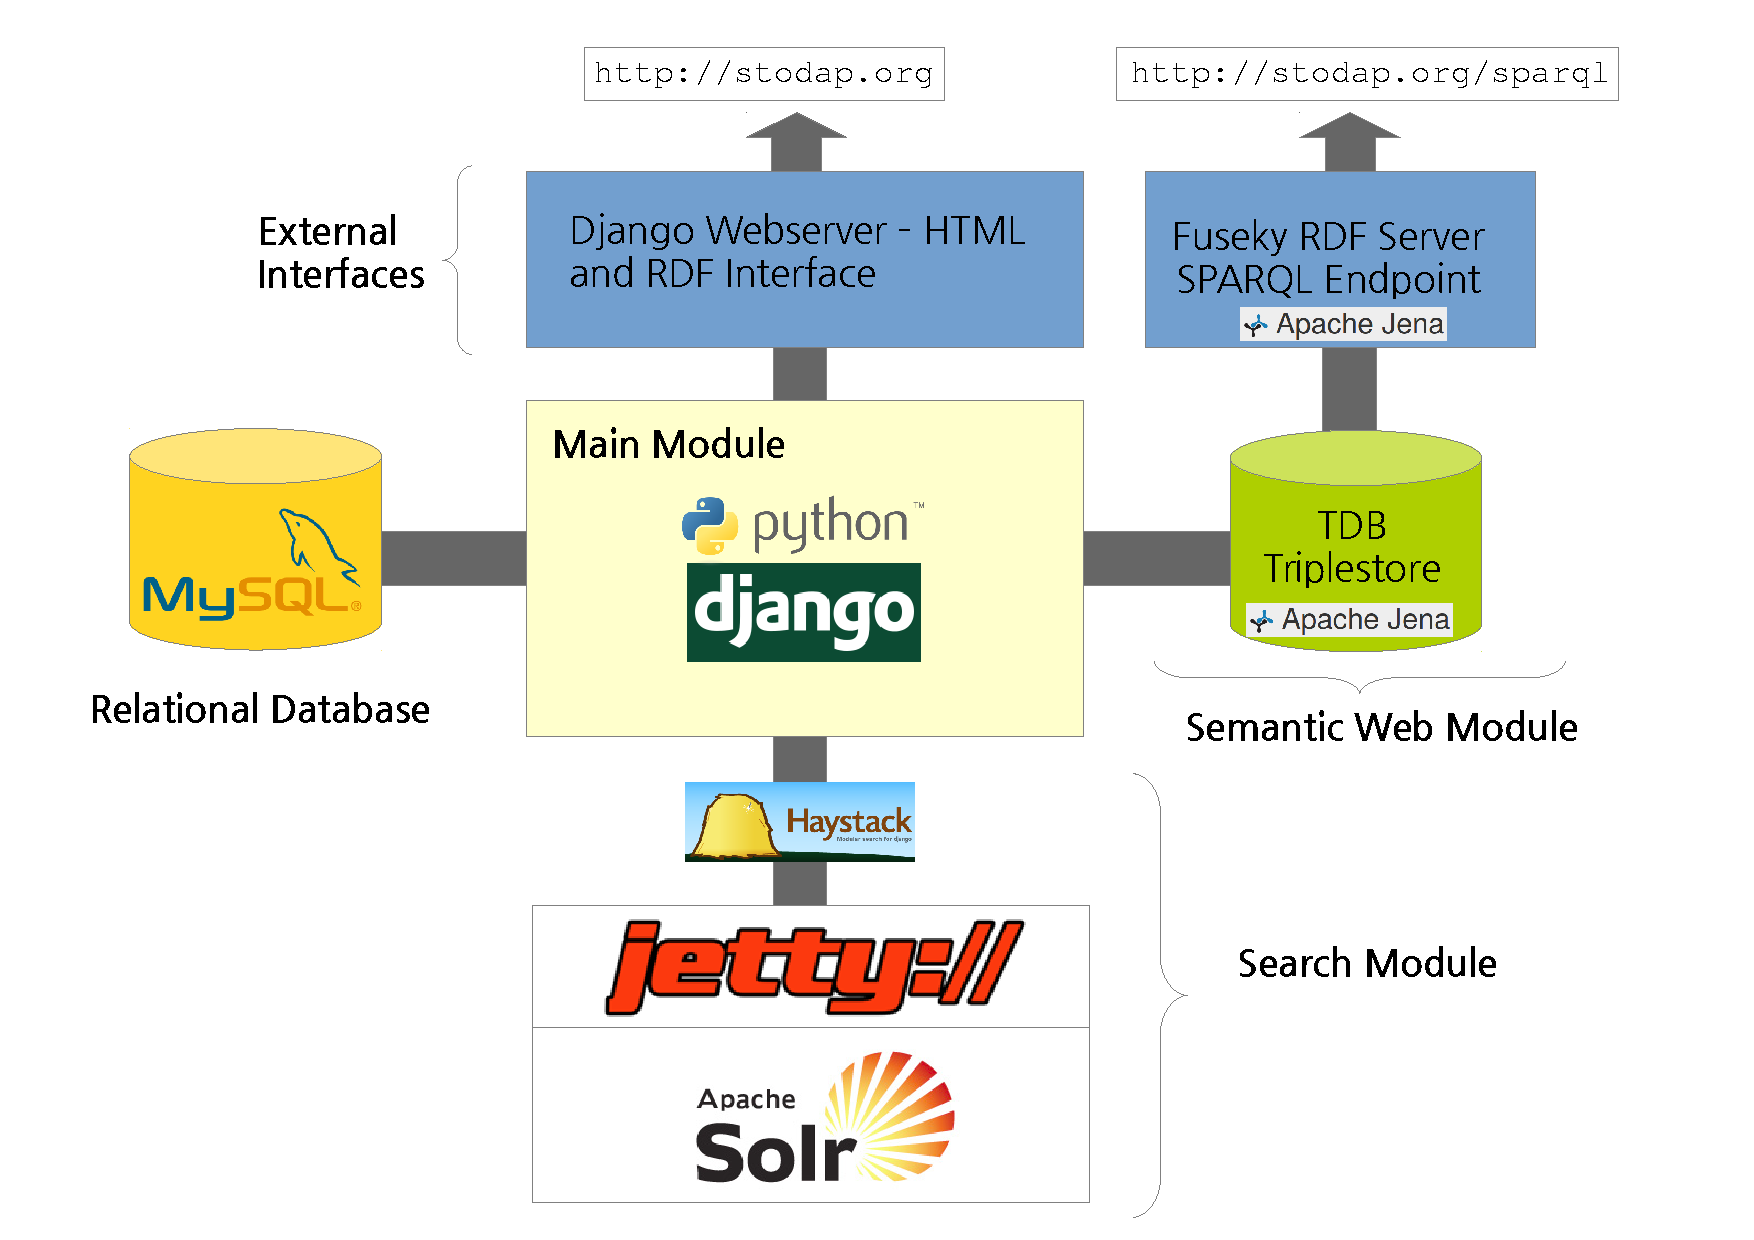
\includegraphics[width=\columnwidth]{images/implementation_architecture.pdf}
\caption[Implementation Architecture of the STODaP approach.]{Implementation Architecture of the STODaP approach.}
\label{fig:implem_arch}
\end{center}
\end{figure}

\subsection{Creating Semantic Tags}

\begin{itemize}
	\item Harvest all tags from portals
	\item Filter significant tags
	\item Group syntactically similar
	\item Translate - lexvo + yandex
	\item Reconcile - lexvo - several ontologies
	\item Choose gemet tags and create semantic tags and links
	\item Create global groups, and reconcile
	\item Associate semantic tags to global groups

	
\end{itemize}

\subsection{CKAN Tag Manager Plugin}

The CKAN Tag Manager one offers an environment for tag curation directly inside the CKAN platform. 
It comprises basic functions such as deletion and editing of tags (not present in CKAN core), and advanced function aimed to enhance the quality of tags.
In this sense, the plugin looks for:
\begin{itemize}
	\item Very similar tags, differing only by capitals or special characters;
	\item Similar tags, with a Levenshtein distance $\le 2$ (after lowercasing and unaccenting)
	\item Possible synonyms, using Natural Language Toolkit~\cite{Bird2009} and the WordNet database.
\end{itemize}
In all those cases, user is offered the option of merging the respective pair of tags.
\autoref{fig:local_curation} shows a screenshot of the CKAN Tag Manager.
The plugin was developed using CKAN API in Python language, and can be installed in any CKAN instance. The source code is available for download and contributions at \url{https://github.com/alantygel/ckanext-tagmanager}.


\begin{figure}[h]
\begin{center}
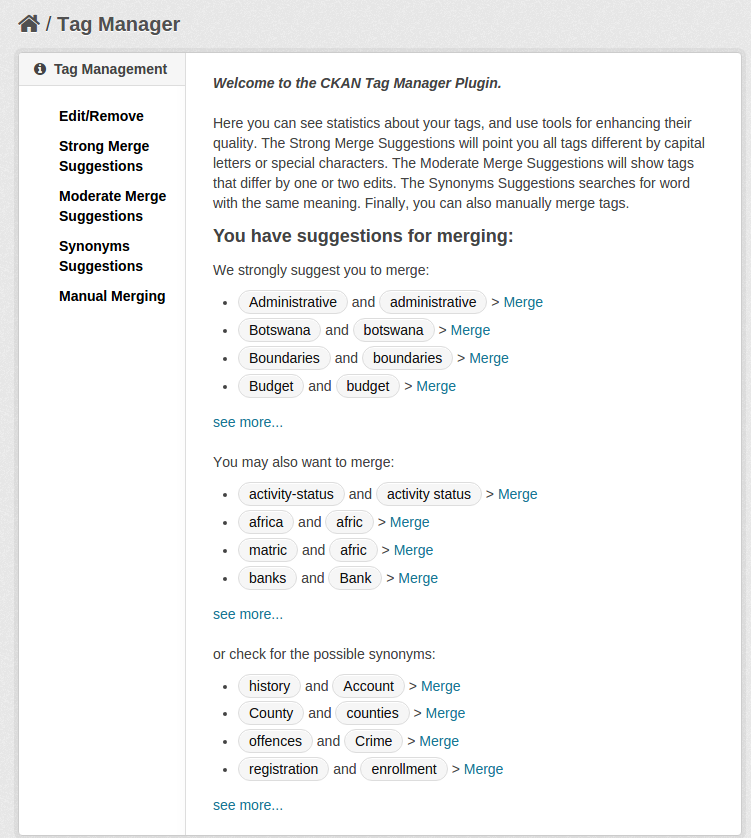
\includegraphics[width=\columnwidth]{images/local_curation.png}
\caption[Screenshot of the Tag Manager plugin.]{Screenshot of the Tag Manager plugin, for tag curation in a CKAN instance. The plugin offers possibilities of manual and semi-automatic tag merging. The first block contains only valid suggestions, while the second block shows 2 false-positives. The synonym module also detected plurals. Tags in this example were extracted from the africaopendata.org portal.}
\label{fig:local_curation}
\end{center}
\end{figure}

\subsection{CKAN Semantic Tags Plugin}

The CKAN Semantic Tags plugin implements the connection between a CKAN instance and the Semantic Tag Server.
Each local tag can be associated to a semantic tag from the server.
After the association, datasets linked with a local tag also point to the global server, as shown in \autoref{fig:local_link}.

\begin{figure}[ht]
\begin{center}
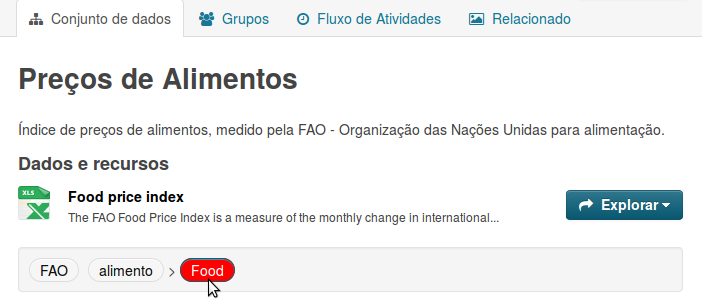
\includegraphics[width=\columnwidth]{images/local_link.png}
\caption[Screenshot of the Semantig Tag plugin.]{Screenshot of the Semantig Tag plugin. The dataset is tagged with two tags, and one of them (\texttt{alimento}) is connected to the semantic tag \texttt{http://stodap.org/tags/Food} through the \texttt{muto:hasTag} property.}
\label{fig:local_link}
\end{center}
\end{figure}

The plugin was developed using CKAN API in Python language, and can be installed in any CKAN instance. The source code is available for download and contributions at \url{https://github.com/alantygel/ckanext-semantictags}.

\subsection{Use and Maintenance of the STODaP server}
\label{sec:use_and_maintenance}

After building the Semantic Tag Server (STODaP), it is necessary to maintain and enhance the tag corpus alongside the evolution of ODPs, as well as to maintain the server updated.
In this subsection, the strategy for it will be presented at the server level.

The first step for building the semantic tag server is to harvest metadata from open data portals.
After the initial setup, a strategy for maintaining the portal up-to-date is needed.

\textbf{Adding a new portal}

When a new ODP is added to the system, a setup procedure is followed:
\begin{itemize}
	\item Harvest tags, datasets and groups metadata;
	\item Clean and group similar tag;
	\item Translate tags, in case of non-English portal;
	\item Reconcile tags with existing Semantic Tags;
	\item If reconciliation is not successful, search lexvo.org and try to create a new semantic tag;
	\item Groups: reconcile with existing global groups or create new ones.
\end{itemize}

\textbf{Updating a portal}

When an ODP is updated, the procedure followed is:
\begin{itemize}
	\item Harvest tags, datasets and groups metadata;
	\item Verify which datasets were inserted or modified
\end{itemize}

%#########################################################################################
\section{Results}
\label{sec:results}
%#########################################################################################

We describe in this section some results achieved with the STODaP approach.
At the global level, it was possible to implement the semantic tags server and to test the performance.
%At the local level it is only possible to claim potential results, as we do not have access to the single ODPs.

\subsection{STODaP Server}

In order to test the system, an open-source implementation of STODaP was created and deployed at \url{http://stodap.org}.
The following approach was used create 663 semantic tags at the server:
\begin{itemize}
	\item From the 220,567 tags harvested, we selected the 663 that were used in more portals, representing all tags used in 10 or more portals; 
	\item Using the Lexvo.org service, we found URI candidates to represent the tag meaning via the \texttt{lexvo:means} property;
	\item Using the Lexvo.org service, we found translations and synonyms for the tags via the \texttt{rdf:seeAlso} and \texttt{lexvo:translate} properties;
	\item We searched for the translations and synonyms in the harvested tags and included the results as \texttt{muto:taggedResources}, together with the portals tagged with the original term;
	\item Using the \href{http://www.nltk.org/}{Natural Language Toolkit  Library}, we searched for semantic similar semantic tags, which were added as \texttt{skos:related}.
\end{itemize}

The occurrence of the original tags among the portals, and the results after including the translations and synonyms can be seen in \autoref{fig:results_tagged_resources}. 
The graphic shows the 30 most used tags, and the achieved increment in the number of relations. 
The occurrence of tags denoting years can also be noticed.
Obviously these tags have no synonyms nor translations, and thus no increment is shown. 
It is also worth mentioning that the tag \texttt{{test}} is the fourth most used one.
This fact is probably related to the early stage of development of some portals. 

\begin{figure}[tb]
\begin{center}
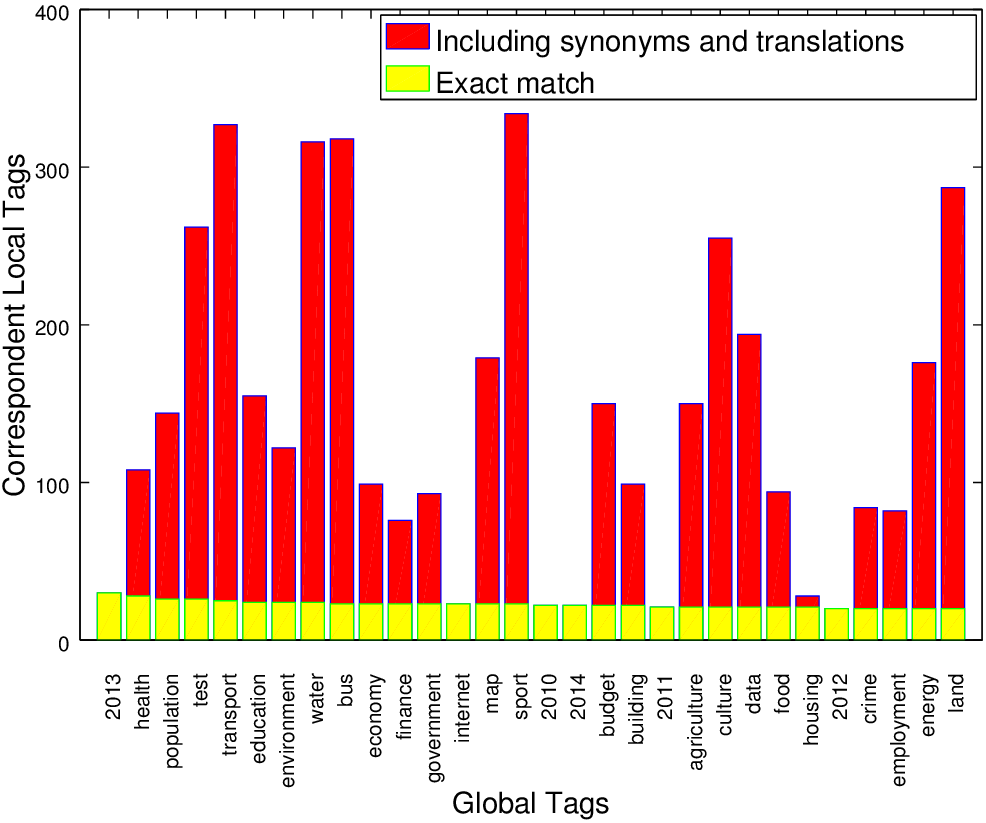
\includegraphics[width=\columnwidth]{images/results_tagged_resources.png}
\caption[Correspondence between local and semantic tags.]{Correspondence between local and semantic tags. The yellow bar shows the number of exact occurrences of the tag in ODPs. The red bar shows the improvement when considered translations and synonyms, which can also occur in a same portal. This explains the numbers over 90. }
\label{fig:results_tagged_resources}
\end{center}
\end{figure}

\subsection{Local Level}

At the local level, the main potential achievements are at the tag curation process.
As shown in \autoref{fig:similarity}, a considerable number of pairs of tags differ only by capital or accented characters.
Using the naive approach to merge similar tags in every portal would result in reducing the number of 14,168 local tags, which represents 6.4\% of the total number of tags.
Lowercase and unaccented tags differing by a Levenshtein-distance from 0 to 2 represent a total of 35,066 pairs, or 15,8\% from the whole tag universe.
However, as discussed above, this approach can lead to false-positives and thus requires manual checking.


%#########################################################################################
\section{Conclusions}
\label{sec:stodap_conclusions}
%#########################################################################################

In this chapter, we presented an approach for metadata reconciliation within and among Open Data Portals.
The use of tags was analysed, and several problems were found, such as a low tag reuse rate and the overall existence of different tags for the same meaning.
On the analysis we also found that several portals share the same tags, showing that tags have a good potential to be linking elements among datasets.
Converting tags into semantic identifiers was also shown as a viable option, even though more sophisticated methods have to be investigated. 
Based on these findings, we derived the STODaP approach, which comprises two parts: 
a local one, aimed at cleaning up and enhancing the quality of ODPs tags, and 
a global one, for connecting ODPs through semantic tags.
The implementation of both shows that significant enhancements can be achieved both at the individual ODPs and the global levels.

Future research and development includes a tag suggestion approach for ODPs which takes into account the related tags at the tag server, using collective knowledge as in~\citeonline{Sigurbjornsson2008}.
Using the possibly structured data of the ODPs in order to improve tagging suggestions is also a research direction that should be followed.
At the global level, an interesting approach is to detect the emergence of schemas from the tags, as described in~\citeonline{Robu2009}.
We will also call for the attention of the open data community in order further to advance collaborative strategies for enriching the tag server.
For STODaP to realize its full potential, ODP administrators and users should be involved and (meta)data literacy needs to be improved.

The ``openness'' of open data is still limited by many factors, including politics, data literacy and technology ones.
With this work, we contributed to the organization and interconnection of ODPs, and thus, given a step further on the enhancement of the open data field.


%1) juntar grupos 
%2) ver quantas tags e datasets estão la dentro
%3) dentro de cada grupo organizar melhor

%Categorization: http://eurovoc.europa.eu/drupal/?q=navigation&cl=en
%Categorization: http://www.eionet.europa.eu/gemet/


%#########################################################################################
\chapter{Evaluation}
%#########################################################################################

In the previous chapter, STODaP approach was presented in details, as well as the supporting tools and their implementation choices.
Practical results were also characterized, showing concrete achievements on the open data organization problem.

In this chapter, the evaluation of STODaP server is described.
The system was compared to other mechanisms on the task of searching for open datasets.
We first present a theoretical background on search engine evaluation methodologies in \autoref{sec:lit_review}.
Then, we show the experimental setup in \autoref{sec:setup} and the results in \autoref{sec:results}.
Some concluding remarks are driven on the final section.

\section{Methodology evaluation background}
\label{sec:lit_review}

As the amount of online available data gets bigger and bigger, search methodologies are increasingly necessary to allow users accessing relevant content.
Thus, it is crucial to develop evaluation techniques that allows researchers to compare different algorithms and find the most adequate ones for each context.

\citeonline{Cheng2010} developed two measures for assessing \emph{user satisfaction} and \emph{user effectiveness} on Interactive Information Retrieval systems.
The first one is called Normalized Task Completion Time (NT), and is calculated as the relation between task completion times for novices and experts.
Following the same reasoning, the Normalized User Effectiveness (NUE) evaluates the relation between relevant documents retrieved by novices and experts, proportional to NT.
Authors claim that this normalization procedure turns the measures more stable against task complexity variations.
Results show that the NT is highly correlated to user satisfaction, while NUE is a better indicator for effectiveness when compared to simple task completion time.
The learning curve was also better explained by NT and NUE than by task completion time.

In a contrary direction, \citeonline{Xu2009} defend the use of task completion time as a robust measure to assess in which extent the search engine helps users to complete a task.
Additionally, these authors found a negative correlation between user satisfaction and task completion time.
An important result of this study is a mathematical development which shows that a cross-over design reduces significantly the variance of the experiment.
Cross-over design means that, when comparing systems A and B on several tasks, every user tests both systems and completes all tasks once, half of them in A, and the other half in B.

%config 1: metade dos usuarios usam um sistema, metade outro, todos fazem todas as tarefas
%config 2: todos fazem todas as tarefas nos dois sistemas > problema : curva de aprendizado - solução - crossover - todos usuarios vao usar os dois sistemas, mas para tarefas diferentes : metade dos usuarios faz metade das tarefas no A e metade no B, e vice-versa

In a survey dealing specifically with faceted search, \citeonline{Wei2013} presents a review about relevance and cost-based metrics on the faceted search context.
Regarding relevance metrics, authors go through a number of works which use precision, recall or F-measure in the same way as on non-faceted search evaluation.
Cost-based metrics look at the time needed to complete a search task, and memory usage.
These metrics were used to compare performance between faceted and non-faceted engines.

Although the Web and search engines have dramatically changed in the last 10 years, the perspective brought by \citeonline{Vaughan2004} is still relevant.
The focus in this work relies on the quality of ranking, i.e., the order in which results are presented.
Both works presented previously rely on the task completion time, which brings with it factors that do not depend on the system, e.g., users ability, and factor not directly related to the search-engine, such as usability.
By looking specifically at the ranking quality, the evaluation methodology may ignore these aspects, and keeps full attention on the search mechanism.
In this work, author proposes non-binary counterparts to the traditional precision and recall measures, with the intention of adding human relevance judgement aspects to the evaluation.
Specifically, two measures are proposed: (i) \emph{Quality of result ranking}, as counterpart of precision and (ii) \emph{Ability to retrieve top ranked pages}, as counterpart measure of recall.
Both measures rely on a human driven ranking of results, which is correlated with the search engine one in the first case.
The second measure evaluates in which extent the top-results are present in each search engine, for the same query.

\section{Experimental Setup}
\label{sec:setup}

% \citeonline{Cheng2010}
% entry questionaire to make sure the users were able to make the test
% novices received a basic training, reading instructions and questions we answered
% The researchers ran a pilot study before finalizing the search tasks to make sure that LexisNexis Academic could retrieve the relevant documents for all these search tasks. Each
% For each search task, the subject stopped the search session when either the information need was satisfied or he or she gave up the task. The researchers observed the subjects performing their searches in order to ensure that the correct procedures were being followed. The researchers also recorded the task completion time of each task, and asked the subjects to answer a questionnaire after each task. As
% 4. Task completion time (T): The time from the start until the completion of a retrieval task. The task completion time is recorded in seconds, but note that the minute was the unit in the calculations. The subjects stopped each search session by themselves, either once their search needs were satisfied or when they gave up.
% 5. User satisfaction (S): An ordinal number indicating the level of user satisfaction. A questionnaire was provided to the users after each search was complete. It asked the subjects to rate their satisfaction level towards the system in regard to supporting the accomplishment of the search task, using a scale from 1 (not satisfied at all) to 5 (extremely satisfied).

In this section, we describe in details our experimental setup.
First of all, we define the evaluation goals:
\begin{itemize}
	\item When searching for open data, how does STODaP compares to other data-specific and general search engines?
	\item What is the usability degree of STODaP server?
\end{itemize}

\subsection{Subjects}

The aim of STODaP server is to facilitate access to open data to the general public.
We consider that experts already have their own strategies and sources for finding adequate data.
Thus, we do not require experience in open data.
However, users must have some previous knowledge on internet navigation. 
Knowledge on basic data processing tools such as spreadsheet processors is also desired, so that subjects can at least imagine a potential use of data.

In our experiment, participants were students attending a class on the topic Information Retrieval at the Federal University of Rio de Janeiro, in Brazil.
An entry-questionnaire was filled by the participants, whose answers are summarized in \autoref{tab:eval_summary}.
Participation was not mandatory and there was no reward for participants.

\begin{table}[]
\ABNTEXfontereduzida
\centering
\caption{STODaP evaluation - summary of subjects profile}
\label{tab:eval_summary}
\begin{tabular}{|p{8cm}|p{2cm}|}
\hline
Participants & \\ \hline
Age & \\ \hline
Internet knowledge (1 - Never Used; 5 - Always use) & \\ \hline
Open Data Experience (1 - Never heard about; 5 - I work often with open data) & \\ \hline
Use of data (1 - I've never used any data processing tool; 5 - I'm an expert in advanced data processing tools) & \\ \hline
\end{tabular}
\end{table}

\subsection{Tasks}

By design, STODaP server is a tool for interlinking different Open Data Portals.
Thus, in this evaluation we aim to assess the ability of gathering similar information from several ODPs, rather than finding specific datasets on the Web.

The evaluation tasks where selected based on: (i) topic relevance of datasets on the open data community, based on criteria defined by Open Data Index\footnote{http://index.okfn.org/} (ii) the existence of search results on STODaP server.
This restriction allows us only to make assertions about the performance of STODaP server on the topics covered by the system, which consists of large base of open data portals, as described in \autoref{sec:stodap_building}.
Broader conclusion would require large scale evaluations, which are over the scope of this thesis.
Defined tasks are:

\begin{itemize}
	\item Find open datasets containing 2015 budget data from locations in 5 different countries.
	\item Find open datasets containing procurement information in 3 different idioms.
	\item Find open datasets about Water Quality on 10 different rivers.
\end{itemize}

\section{Procedure}

The following procedure was driven during the evaluation process:

\begin{itemize}
	\item Participants filled the entry-questionnaire (5 minutes);
	\item The main idea of the project was explained, followed by an explanation about (10 minutes)
	\item Participants were assigned numbers and asked to enter this number on the form. 
	\item Three tasks were sequentially presented. 
	Each one was demanded to be completed either using STODaP server, the Exversion Data Search Engine\footnote{Available at \url{https://www.exversion.com/search/}} or conventional search engines \cite{Xu2009}.
	The combination between search method, task and ordering was randomly chosen for participants.
	\item For each task, the challenge was presented with the appropriate number of text fields for pasting the results links.
	\item The time taken for each task was automatically calculated. The search string used in STODaP server were also captured.
	\item An evaluation questionnaire was filled by the subjects, containing questions about usability and satisfaction.
\end{itemize}

\section{Pre-Evaluation}
In order to test and adjust our evaluation setup, we ran the process with a group of seven students of an Information Retrieval graduate course, at the Federal University of Rio de Janeiro.
The results of this first round can be seen in \autoref{tab:pre_eval_questionnaire} and \autoref{tab:pre_eval_results}.
Although the main target of this pre-evaluation process was to assess the evaluation procedure (and not the STODaP server), it is useful to look at the results to have the first impressions.

\begin{table}[h]
\ABNTEXfontereduzida
\centering
\caption[Answers to the entry and evaluations questionnaires.]{Answers to the entry and evaluations questionnaires. The first four questions correspond to the entry-questionnaire, applied before the evaluation. The two remaining questions were answered after completing the evaluation tasks.}
\label{tab:pre_eval_questionnaire}
\begin{tabular}{|>{\centering\arraybackslash}m{.5cm}|>{\centering\arraybackslash}m{.8cm}|>{\centering\arraybackslash}m{1.cm}|>{\centering\arraybackslash}m{.8cm}|>{\centering\arraybackslash}m{.8cm}|>{\centering\arraybackslash}m{2cm}|>{\centering\arraybackslash}m{3cm}|>{\centering\arraybackslash}m{3cm}|}
\hline
& 	Age & Internet Ability (1 - low; 5 - high) & Data Ability (1 - low; 5 - high) & Open Data Ability  (1 - low; 5 - high) &	Do you think STODaP is a useful tool for finding data on the web?  (1 - not useful; 5 - very useful) &	How easy is it was get the data you need using the STDOaP in comparison with the other methods?  (1 - harder; 5 - easier) & 	Average TCT (seconds) \\ \hline
1& 	27& 	5& 	3& 	1& 	4& 	2& 	295.7 +/- 98.8 \\ \hline
2& 	23& 	5& 	4& 	3& 	5& 	3& 	833.3 +/- 151.8 \\ \hline
3& 	27& 	5& 	5& 	5& 	2& 	2& 	560.0 +/- 103.2 \\ \hline
4& 	23& 	5& 	4& 	3& 	5& 	4& 	845.0 +/- 523.9 \\ \hline
5&	26& 	5& 	3& 	2& 	5& 	5& 	625.3 +/- 269.5 \\ \hline
6& 	29& 	5& 	5& 	3& 	4& 	4& 	527.0 +/- 287.5 \\ \hline
7& 	22& 	5& 	4& 	1& 	5& 	5& 	351.0 +/- 121.2 \\ \hline
\end{tabular}
\end{table}

\begin{table}[]
\ABNTEXfontereduzida
\centering
\caption[Task Completion Time of the pre-evaluation test, in seconds.]{Task Completion Time of the pre-evaluation test, in seconds. 
Each cell contains the number of seconds that one or more subjects took to complete the task with the correspondent search method.}
\label{tab:pre_eval_results}
\begin{tabular}{|p{2.5cm}|p{2.5cm}|p{2.5cm}|p{2.5cm}|p{2.5cm}|}
\hline
\textbf{Tasks / Search Methods} & \textbf{Water Quality} & 	\textbf{Budget information} &	\textbf{Procurement} &	\textbf{Average and Standard Deviation} \\ \hline
\textbf{Exversion} &	723, 884, 468 &	235, 382 &	558, 518 &	538.3 +/- 198.5 \\ \hline
\textbf{STODaP} &	435, 493, 460 &	397, 184, 517, 1048 & -	&	504.9 +/- 244.0 \\ \hline
\textbf{Free} &	1580 &	702 &	401, 217, 180, 1001, 729 &	687.1 +/- 456.3 \\ \hline
\textbf{Average and Standard Deviation} &	720.4 +/- 383.7 &	495.0 +/- 276.7 &	514.9 +/- 266.7 &\\ \hline
\end{tabular}
\end{table}

\autoref{tab:pre_eval_questionnaire} shows the answers of each subject to the questions both before and after running the evaluation.
As expected, all subjects are frequent internet users.
Use of data in daily work or study is also high, but the only one declared himself an open data expert.
Coincidently or not, this subject was the only who did not considered STOaP an useful tool for finding data on the web.
Four out of seven considered that completing the tasks with STODaP was easier than with other methods.
The average Task Completion Time had a huge variation, with a minimum of 295 seconds and a maximum of 845 seconds.

\autoref{tab:pre_eval_results} shows the Task Completion Times for each task and search method.
We can easily notice that a choosing a random generator for attributing tasks, search methods and orders was a mistake, specially with a small number of rounds.
There were 36 possibilities (6 orderings for tasks $\times$ 6 orderings for search methods) but only 7 rounds were used.
Thus, the number of combinations between tasks and search methods ended up quite unbalanced, and there was no combination of STODaP search method with the procurement task.

After running the procedure, a conversation round was driven with the students on order to get insights both about the tool and the evaluation procedure.
The following suggestions and comments were made:

Regarding the evaluations interface:

\begin{itemize}
	\item Alert that search engines should be open in another tab;
	\item Write the tasks more clearly and specific (e.g., asking budget 2015 may include 2014-16?)
	\item On the final questions, positive answers to the system were at the left side, which is not usual and confused some subjects;
	\item State more clearly that only the link to the dataset should be answered;
	\item Makes clear that users are allowed to use auxiliary tools such as translators or Wikipedia in order to better understand the tasks;
	\item State more clearly that users should only look to the dataset title, and there is no need to open it;
	\item Explain that only some specific portals are indexed, not all open data in the world.
\end{itemize}

Regarding the evaluations procedure:
\begin{itemize}
	\item On the evaluation questionnaire, ask the English proficiency and other languages, and ask if the English language hampered the performance;
	\item To few questions - do not evaluate learning curve.
\end{itemize}
	
Regarding the STODaP faceted search interface:
\begin{itemize}
	\item There should be an explanation about faceted search and how does it work;
	\item Regarding the Portal facet, it was suggested to write portals name in spite of url, when this metadata is available
	\item One participant reported that he took a while to realize the language facet; after seeing it, it was very quick.
	\item It was suggested to include the possibility of making the query broader by including facets with OR.
\end{itemize}	

There were some positive comments:
\begin{itemize}
	\item It was noted that results presented by STODaP had a higher quality in relation to Exversion, mainly because the latter automatically uses an OR logic between two terms.
	This results in many unwanted outputs.
	\item The possibility of searching English keywords and getting multi-language results was also positively mentioned, because no other tool presents such feature.
	\item The STODaP interface, in its search results, exhibits datasets with all its tags.
	This was positively noted, because it helps to decide quicker if a dataset is of interest or not.
\end{itemize}	

Analysing students while they were completing their tasks was also show some new perspectives.
It was noticed that some subjects tried to look deep at datasets in order to verify if they met the task criteria.
It should be harder stressed in the explanation that this is not necessary, since the our objective is only to find dataset, and not to verify their quality.
Some students tried to use analytic tools such as Google Public Data.
Their focus is rather on analysing (open) data sets than on making them available for download in machine readable formats.
Thus, for our intentions, this is not considered open data and it should also be stated in the explanation.


\section{Results}
\label{sec:eval_results}


\subsection{Validation}
Each entry-questionnaire was analysed in order to determine if it is valid to our evaluation, in terms of internet experience.

The answers were also checked in order to confirm if the dataset links provided are really valid answers to the assigned task.

\subsection{Analysis}
\begin{itemize}
	\item Task completion time for each task (and variance) \cite{Xu2009}
	\item Task completion time for each search method (and variance) \cite{Xu2009}
	\item Correlation between satisfaction and completion time for STODaP server \cite{Xu2009}
	\item Correlation between results found in the different search methods \cite{Vaughan2004}

\end{itemize}


\section{Conclusions}
\label{sec:conclusion}



% The main objective of the STODaP approach is to facilitate the access of open data by the general public.
% Thus, in order to test our approach we defined an use case.

% John is a journalist.
% He has to write an article about openness of health data around the world.
% Apart of writing about specific cases using national reports, he want's to give the readers a global overview.
% His first approach is to access search engines.
% However, he faces hundreds of open data portals, in different languages, which turns the task of retrieving health data into a difficult task.
% Using the STODaP server, John is able to access datasets of 87 open data portals related to the concept of health, and also other connected concepts.



\chapter{Conclusions}
\label{chap:conclusions}
% gancho para motivação e objetivos; introduir o assunto com um pouco mais de profundidade

% 1) enfatizar contribs
% --> falar dos resultados especificose limitaçẽis do experimento; aqui tem que generalizar se possível
% 2) falar de limitações e dificuldades
% 3) trabalhos futuros
% 4-8 de julho

% amarração do Data literacy; o experiemento teve a ver com data litearcy
% enfatizar nas limitações que o grupo do DL deveria ter sido o teste stodap

The open data promises are still far from being materialised.
However, it cannot be denied that significant advances have been made in recent years.
In this section, the conclusions of this thesis will be derived, based on the initial hypothesis and in the developments that were made during this work.

\section{Contributions of this Work}

In the Introduction of this work, two hypothesis were posed, which, for the ease of reading, are reproduced here:

\noindent\textbf{H\ref{hyp:dataliteracy}:} Increasing the level of data literacy on the society leads to a more conscious use of open data.

\noindent\textbf{H\ref{hyp:tagging}:} Enhancing the organization of open data repositories leads to better find ability of open data.

The work towards validating H\ref{hyp:dataliteracy} was described in \autoref{chap:dataliteracy}.
The importance of data literacy efforts was enforced in \autoref{dl_paulofreire}, where an analogy between traditional and data literacies was derived.
We concluded showing the importance of data literacy on giving voice to marginalized people, in the same way as it was crucial to alphabetise people some decades ago.
A definition of the concept of \emph{Critical Data Literacy} was also presented, emphasizing the need of a real understanding of what is behind data.
In \autoref{dl_method} our proposal for working on data literacy with social movements activists was presented.
A methodology for data literacy course was detailed, mixing theory, discussion and practice, in an effort to bring data literacy knowledge closer to each educands reality.

Our hypothesis H\ref{hyp:dataliteracy} was partially validated in \autoref{dl_results}, where the results of the application of this course were presented.
Specially, in \autoref{fig:dl_results}, we depicted the critical apprehension of data literacy course participants regarding the problems of open data.
Tables~\ref{tab:dl_results1}, \ref{tab:dl_results2}, and \ref{tab:dl_results3} complement the diagram and present in a more detailed form the outputs of the data literacy course.
The critical use of data by subjects, however, could not be evaluated.
As discussed in \autoref{sec:obs_based_analysis}, the fourth stage of the course, were the real use of data was planned, was reached only twice, and thus it would be precipitated to take any conclusions about it.

Regarding H\ref{hyp:tagging}, the first chapters of this thesis emphasized the importance of open data in our society, and we showed by literature review (\autoref{sec:problems}), participatory research (\autoref{dl_results}) and objective metrics (\autoref{sec:analysis}) that organizing open datasets is a relevant problem.
The STODaP approach proposed in \autoref{chap:tagging} targeted precisely the open data organization problem, both from a local perspective (inside a single ODP) and from a global perspective (inter-ODPs).
Our STODaP server, an updated metadata repository, was tested in the previous chapter, and results shown that system helped people in finding the more datasets quicker than using traditional approaches.
This can be considered true specially for non-experts in open data.

\subsection{Generalisation}

In order to validate both hypothesis, general theoretical and practical analysis were developed.
However, experiments are intrinsically specific.
Thus, it is necessary to discuss if the results described in this thesis can be generalised, or if they are true only for a specific context.

Regarding the results achieved by the data literacy experiment, the specificity lies in the main characteristic of the participants, i.e., social movements activists.
Although the open data impediments gathered on the course do not differ substantially from others reported on the literature, we can see that motivations and desired improvements are very specific of social movements activities.

Thus, we can affirm that:

\noindent \emph{The developed data literacy course methodology was able to raise critical impediments, motivations and improvements on social movement activists. However, the use of open data by theses subjects could not be tested.}

As discussed in the conclusions of the last chapter, the evaluation of STODaP server has two specific design choices that may affect the generality of the results.
The first aspect is the choice of subjects.
Participants of the experiment can be divided in three groups: (i) first year Computer Sciences students, in Brazil; (ii) Semantic Web researchers of various nationalities; (iii) open data practitioners/activists in Brazil.
Even though there are significant variations on the level data/open data experience among these subjects, all of them share a daily use of internet and a good English proficiency.

The second design choice were the tasks that subjects had to complete: (i) find 2015 open budget data from 5 countries; (ii) Find open data about water quality in seven rivers outside Europe; and (iii) find open procurement datasets in 3 different languages.
The choice of these 3 topics was based on the 13 criteria used by the Open Data Index\footnote{The Open Data Index compiles an open data ranking, whose criteria are: National Statistics, Government Budget, Legislation, Procurement tenders, Election Results, National Map, Weather forecast, Pollutant Emissions, Company Register, Location datasets, Water Quality, Land Ownership and Government Spending. For each of these topics, countries are evaluated and receive a score according to openness level.}, in order to guarantee the relevance of tasks.

In this context, it is not possible to guarantee the extension of our results to subjects not from the Computer Science field, with a low English proficiency, or with a low Computer/Internet ability.
Regarding the topics, since all Open Data Index topics have a significant amount of open datasets, it is secure to generalize our findings to other relevant open data topics.

Thus, we can affirm that:

\noindent \emph{For users with an intermediate level of English and some approximation to the Computer Science field, STODaP open data search engine delivers open dataset with more quality in less time than other search methods when searching for relevant open data topics.}

\section{Problems and Limitations}

After highlighting the contributions of this thesis, it is also necessary expose some problems and delimit the extension of our results.

First of all, by choosing the problem of open data organization, we left several other ones detected on \autoref{chap:dataliteracy} open.
It is of course impossible to deal with every problem on the open data field, but some of them are of crucial importance, as for example the Data Quality problem.
In our evaluation procedure, subjects went only to the entry point of datasets.
It is possible that datasets that were marked as valid in the evaluation do not correspond to their descriptions, are outdated, or have broken links to their resources.
This is a clear limitation of this work: open datasets search is based on metadata, but data quality cannot be guaranteed.

Another limitation of the approach is related to the subjects that participated on the evaluation.
Ideally, we would like that the same subjects that attended to the Data Literacy course could evaluate the system.
However, this was not possible, mainly because: (i) Most of the participants on the Data Literacy course do not speak English; (ii) the time span between the courses and the evaluation was of almost 2 years, which makes contacts more difficult.
Thus, it was not possible to evaluate if the developed system attended to at least some of the requirements pointed out by participants of the courses.

The connection between tags and semantic tags is also limited by the moment.
The automatic approach used in this thesis resulted in many tags not connected to right semantic tag, and also many wrong connections. 
Although several methods to tackle this issue are available in the literature, the large size of our database requires efficient approaches.


\section{Future Works}

The broadness of this work let many open paths for further research.

On the Data Literacy field, \autoref{fig:dl_results} can give relevant clues for further research.
The training branch presents a great variety of topics, ranging from Basic Informatics, Mathematics and Statistics, until data journalism or open data publishing.
The possibility of integrating such a wide range of topics in Data Literacy courses should be further investigated.

Regarding reconciliation of tags in ODPs, a sort of crowd validation would be very useful in order to confirm automatic processing and add new information.
The model proposed by \citeonline{Limpens2013} could be very useful, because of its ability to deal with divergences between users.
In this sense, it is necessary to call the attention of the open data community in order further to advance collaborative strategies for enriching the semantic tags server.

Another way of improving the connection between tags and groups with their semantic equivalents could be via artificial intelligence methods. 

Advances on local tools for tagging assistance are crucial, since a good tagging procedure would certainly ease the work of tag reconciliation. 
Future research and development should include a tag suggestion approach for ODPs which takes into account the related tags at the tag server, using collective knowledge as in~\citeonline{Sigurbjornsson2008}.
Using the possibly structured data of the ODPs in order to improve tagging suggestions is also a research direction that should be followed.

Another interesting research direction is the detecting the emergence of schemas from the tags, as described in~\citeonline{Robu2009}, where tag correlation is used to create tagging vocabularies and visualizations of terms relationships.

The STODaP system also need a more professional approach on its development in order to be really useful. A priority list of enhancements could start by: 

\begin{itemize}
	\item Internationalization. At the moment, semantic tags and groups labels are only in English. This means that users searching for keywords in English are able to find datasets in other languages via semantic tags, but the contrary is not true. The Gemet Thesaurus offers several translations of the terms, which could be used for this task.
	\item User Interface Design. Several subjects commented on the evaluation that interface design should be improved. This is a priority because interface problems can hide system functionalities, and thus result in a worse performance than the system could offer.
	\item Include other open data portals. The list of ODPs indexed by the STODaP server came from the CKAN Census. The first problem is that this Census is not frequently updated, since many CKAN ODPs listed there do not exist more, and other not present in the Census were found. Secondly, a great quantity of ODPs are developed using Socrata, another open data management system. Although being proprietary, Socrata also offers APIs for external users to consume data. Developing the interface between CKAN and Socrata could significantly improve the STODaP base.
\end{itemize}

\vspace{1cm}
\begin{center}* * *
\end{center}
\vspace{1cm}

For STOdAP to realize its full potential, ODP administrators and users should be involved and (meta)data literacy needs to be improved.	
The ``openness'' of open data is still limited by many factors, including politics, data literacy and technology ones.
With this work, we hope to have contributed to the open data field, maybe no so much with the resulting tool, but hopefully with a socio-technical view where the user side can have at least the same importance as the publisher side.

% ----------------------------------------------------------
% ELEMENTOS PÓS-TEXTUAIS
% ----------------------------------------------------------
\postextual
% ----------------------------------------------------------

% ----------------------------------------------------------
% Referências bibliográficas
% ----------------------------------------------------------
\bibliography{bib/pb-bibliography,bib/bibliography,bib/referencias,bib/abntex2-modelo-references}
% ----------------------------------------------------------
% Glossário
% ----------------------------------------------------------
%
% Consulte o manual da classe abntex2 para orientações sobre o glossário.
%
%\glossary

% ----------------------------------------------------------
% Apêndices
% ----------------------------------------------------------

% ---
% Inicia os apêndices
% ---
\begin{apendicesenv}

% Imprime uma página indicando o início dos apêndices
\partapendices

%\begin{englishabstract}{Colocar aqui o título da dissertação em inglês}{coloque aqui as palavras-chave em inglês, separadas por vírgula}

%\begin{listofpublications}{}
\chapter{List of Publications}

\section{Peer-reviewed conferences}
\begin{itemize}

\item TYGEL, A. F.; AUER, S.; DEBATTISTA, J., ORLANDI, F.; CAMPOS, M. L. M. . Towards Cleaning-up Open Data Portals: A Metadata Reconciliation Approach. To be presented at the 10th International Conference on Semantic Computing, Laguna Hills, California. February 3-5 2016.

\item TYGEL, A. F.; ATTARD, J.; ORLANDI, F.; CAMPOS, M. L. M. ; AUER, S. . "How much?" Is Not Enough - An Analysis of Open Budget Initiatives. To be presented at ICEGOV 2016, Montevideo, March 1-3 2016.

\item TYGEL, A. F. ; KIRSCH, R. . Contributions of Paulo Freire for a Critical Data Literacy. In: Data Literacy Workshop, 2015, Oxford. Proceedings of the Data Literacy Workshop, 2015. 

\item CARVALHO, L. ; RODRIGUES, F. ; FERREIRA, R. ; BRAGA, P. ; TYGEL, A. F. ; ALVEAR, C. A. S. ; PRIMO, R. . Software Livre e Metodologias Participativas - ensino e extensão em uma disciplina da Engenharia. In: Encontro Nacional de Engenharia e Desenvolvimento Social - ENEDS, 2015, Salvador. Anais do XII ENEDS, 2015.

\end{itemize}

\section{Peer-reviewed journals}
\begin{itemize}

\item TYGEL, A. F. ; LUIZA MACHADO CAMPOS, MARIA ; ALVEAR, C. A. S. . Teaching Open Data for Social Movements: a Research Strategy. Journal of Community Informatics, v. 11, p. 1, 2015.

\item TYGEL, ALAN ; GONÇALVES, LEONARDO GONÇALVES ; SANTOS, MAYARA ; MARQUES, GABRIEL ; LUIZA MACHADO CAMPOS, MARIA . Informação para Ação: Desenvolvimento de um Portal de Dados Abertos Sobre Agrotóxicos. Revista Tecnologia e Sociedade, v. 11, p. 99-119, 2015. 
\end{itemize}

\section{Book chapters}
\begin{itemize}
\item TYGEL, A. F. ; Tecnologias da Informação e Comunicação e Movimentos Sociais: o Caso da Cooperativa EITA. In: Felipe Addor e Flávio Chedid. (Org.). Tecnologia, Participação e Território - Reflexões a partir da Prática Extensionista. 1ed.Rio de Janeiro: Editora UFRJ / Faperj, 2015, v. 3, p. 259-292.
\end{itemize}

%\end{listofpublications}


\chapter{Results of Open Data Research}

%\begin{table}[htb]
%\ABNTEXfontereduzida
%\caption[Níveis de investigação]{Níveis de investigação.}
%\label{tab-nivinv}
%\begin{tabular}{p{2.6cm}|p{6.0cm}|p{2.25cm}|p{3.40cm}}
%  %\hline
%   \textbf{Nível de Investigação} & \textbf{Insumos}  & \textbf{Sistemas de Investigação}  & \textbf{Produtos}  \\
%    \hline
%    Meta-nível & Filosofia\index{filosofia} da Ciência  & Epistemologia &
%    Paradigma  \\
%    \hline
%    Nível do objeto & Paradigmas do metanível e evidências do nível inferior &
%    Ciência  & Teorias e modelos \\
%    \hline
%    Nível inferior & Modelos e métodos do nível do objeto e problemas do nível inferior & Prática & Solução de problemas  \\
%   % \hline
%\end{tabular}
%\legend{Fonte: \citeonline{van86}}
%\end{table}


%Já a \autoref{tabela-ibge} apresenta uma tabela criada conforme o padrão do
%\citeonline{ibge1993} requerido pelas normas da ABNT para documentos técnicos e
%acadêmicos.

%\begin{table}[htb]
%\IBGEtab{%
%  \caption{Um Exemplo de tabela alinhada que pode ser longa
%  ou curta, conforme padrão IBGE.}%
%  \label{tabela-ibge}
%}{%
%  \begin{tabular}{ccc}
%  \toprule
%   Nome & Nascimento & Documento \\
%  \midrule \midrule
%   Maria da Silva & 11/11/1111 & 111.111.111-11 \\
%  \midrule 
%   João Souza & 11/11/2111 & 211.111.111-11 \\
%  \midrule 
%   Laura Vicuña & 05/04/1891 & 3111.111.111-11 \\
%  \bottomrule
%\end{tabular}%
%}{%
%  \fonte{Produzido pelos autores.}%
%  \nota{Esta é uma nota, que diz que os dados são baseados na
%  regressão linear.}%
%  \nota[Anotações]{Uma anotação adicional, que pode ser seguida de várias
%  outras.}%
%  }
%\end{table}



\begin{table}[]
\ABNTEXfontereduzida
\caption{Motivations, Impediments and Improvements indicated in answers to Question 4.}
\label{tab:dl_results1}
\begin{tabular}{|p{1cm}|p{4.4cm}|p{4.4cm}|p{4.4cm}|}
%\begin{tabular}{|l|l|l|l|}
\hline
\multicolumn{4}{|l|}{Question 4: Why have you attended to the course? Why do you think open data is important?} \\ \hline
\multicolumn{1}{|c|}{\textbf{\#}} & \multicolumn{1}{c|}{\textbf{Motivations}}                                                                       & \multicolumn{1}{c|}{\textbf{Impediments}}                                                                                                               & \multicolumn{1}{c|}{\textbf{Improvements}} \\ \hline
4.1&Work with data and link different information to create arguments&There is a mismatch between amount of data released and the capacity of social movements to analyse it &Make investments in education for open data use\\ \hline
4.2&Be able to work with data driven journalism&There are many barriers to access information&Promote publicity about existence of data\\ \hline
4.3&Use data to denounce injustices&Open Data is unknown for most social movements&Improve knowledge about how to search for data\\ \hline
4.4&Data can give basis to stimulate new claims &There is no full transparency in government actions&Enable access to information, without discrimination\\ \hline
4.5&Translate data into information for readers&Most of the people have little informatics ability&\\ \hline
4.6&Produce data in juridical research&&\\ \hline
4.7&Open data can stimulate analysis&&\\ \hline
4.8&Open data can stimulate new data&&\\ \hline
4.9&Validate/legitimate arguments in communication with data&&\\ \hline
4.10&Use data to understand the capitalist society&&\\ \hline
4.11&Understand the resistances against oppression with data&&\\ \hline
4.12&Fight corruption using spending data &&\\ \hline
4.13&Make better use of information, a central point in class conflicts&&\\ \hline
4.14&Unveil data manipulation&&\\ \hline
\end{tabular}
\legend{Source: \citeonline{Tygel2015a}}
\end{table}


\begin{table}[]
\ABNTEXfontereduzida
\caption{Impediments pointed in answers to Question 8.}
\label{tab:dl_results2}
\begin{tabular}{|l|l|}
\hline
\multicolumn{2}{|l|}{Question 8: What is the main impediment perceived by using data?}                                       \\ \hline
\multicolumn{1}{|c|}{\textbf{\#}} & \multicolumn{1}{c|}{\textbf{Impediments}}                                                \\ \hline
8.1                               & The lack of knowledge about data production process makes interpretation difficult       \\ \hline
8.2                               & It is hard to understand data connection and linking possibilities                       \\ \hline
8.3                               & Finding data in the web is hard /Open data portals are complicated                       \\ \hline
8.4                               & Access to data outside the web is hard / FoIA application is complicated                 \\ \hline
8.5                               & Data organization is confused                                                            \\ \hline
8.6                               & Data formats does not help its use                                                       \\ \hline
8.7                               & The state presents data through different platforms which increase the need for training \\ \hline
8.8                               & The need of specific software tools makes data usage harder                              \\ \hline
8.9                               & Some important data is concealed                                                         \\ \hline
8.10                              & Most data is outdated                                                                    \\ \hline
8.11                              & The querying interfaces present too much information                                     \\ \hline
8.12                              & Access to raw data is hard                                                               \\ \hline
8.13                              & Government agencies do not follow common data standards                                  \\ \hline
8.14                              & "Data interpretation is difficult                                                        \\ \hline
8.15                              & Linking data from different sources is difficult without appropriate tools and metadata  \\ \hline
\end{tabular}
\legend{Source: \citeonline{Tygel2015a}}
\end{table}


\begin{table}[]
\ABNTEXfontereduzida
\caption{Improvements indicated in answers to Question 9.}
\label{tab:dl_results3}
\begin{tabular}{|l|l|}
\hline
\multicolumn{2}{|l|}{Question 9: How do you imagine that the use of data could be improved?}           \\ \hline
\multicolumn{1}{|c|}{\textbf{\#}} & \multicolumn{1}{c|}{\textbf{Improvements}}                         \\ \hline
9.1                               & Provide user-friendly interfaces                                   \\ \hline
9.2                               & Provide education on statistics/mathematics                        \\ \hline
9.3                               & Standardize open government data                                   \\ \hline
9.4                               & Provide user-friendly language (avoid technical terms)             \\ \hline
9.5                               & Provide wider training possibilities                               \\ \hline
9.6                               & Promote more advertising of open government data initiatives       \\ \hline
9.7                               & Promote more advertising of social movements open data initiatives \\ \hline
9.8                               & Foster more research on open data and social movements             \\ \hline
9.9                               & Improve data search engines                                        \\ \hline
9.10                              & Increase the offer of open data sources                            \\ \hline
9.11                              & Avoid the need of intermediaries for data interpretation           \\ \hline
9.12                              & Improve open data portals                                          \\ \hline
\end{tabular}
\legend{Source: \citeonline{Tygel2015a}}
\end{table}



\end{apendicesenv}
% ---



%---------------------------------------------------------------------
% INDICE REMISSIVO
%---------------------------------------------------------------------
\phantompart
\printindex
%---------------------------------------------------------------------

\end{document}
